%% FEUP THESIS STYLE for LaTeX2e
%% how to use feupteses (English version)
%%
%% FEUP, JCL & JCF, 31 July 2012
%%
%% PLEASE send improvements to jlopes at fe.up.pt and to jcf at fe.up.pt
%%

%%========================================
%% Commands: pdflatex tese
%%           bibtex tese
%%           makeindex tese (only if creating an index) 
%%           pdflatex tese
%% Alternative:
%%          latexmk -pdf tese.tex
%%========================================

\documentclass[11pt,a4paper,twoside,openright]{report}

%% For iso-8859-1 (latin1), comment next line and uncomment the second line
\usepackage[utf8]{inputenc}

%\usepackage[latin1]{inputenc}

%% English version

%% MIEIC options
%\usepackage[mieic]{feupteses}
\usepackage[mieic,juri]{feupteses}
%\usepackage[mieic,final]{feupteses}
%\usepackage[mieic,final,onpaper]{feupteses}

%% Additional options for feupteses.sty: 
%% - onpaper: links are not shown (for paper versions)
%% - backrefs: include back references from bibliography to citation place

%% Uncomment the next lines if side by side graphics used
%\usepackage[lofdepth,lotdepth]{subfig}
%\usepackage{graphicx}
%\usepackage{float}

\usepackage{amsmath}
\usepackage{float}
\usepackage{wrapfig}
\usepackage{subfig}
\usepackage{longtable}
\usepackage{multirow}
\usepackage{pdfpages}
\usepackage{fancyhdr}
\pagestyle{fancy}

%% Include color package
\usepackage{color}
\definecolor{cloudwhite}{cmyk}{0,0,0,0.025}

%% Include source-code listings package
\usepackage{listings}
\lstset{ %
 language=C,                        % choose the language of the code
 basicstyle=\footnotesize\ttfamily,
 keywordstyle=\bfseries,
 numbers=left,                      % where to put the line-numbers
 numberstyle=\scriptsize\texttt,    % the size of the fonts that are used for the line-numbers
 stepnumber=1,                      % the step between two line-numbers. If it's 1 each line will be numbered
 numbersep=8pt,                     % how far the line-numbers are from the code
 frame=tb,
 float=htb,
 aboveskip=8mm,
 belowskip=4mm,
 backgroundcolor=\color{cloudwhite},
 showspaces=false,                  % show spaces adding particular underscores
 showstringspaces=false,            % underline spaces within strings
 showtabs=false,                    % show tabs within strings adding particular underscores
 tabsize=2,	                    % sets default tabsize to 2 spaces
 captionpos=b,                      % sets the caption-position to bottom
 breaklines=true,                   % sets automatic line breaking
 breakatwhitespace=false,           % sets if automatic breaks should only happen at whitespace
 escapeinside={\%*}{*)},            % if you want to add a comment within your code
 morekeywords={*,var,template,new}  % if you want to add more keywords to the set
}

%% Uncomment to create an index (at the end of the document)
%\makeindex


%% Path to the figures directory
%% TIP: use folder ``figures'' to keep all your figures
\graphicspath{{figures/}}

%%----------------------------------------
%% TIP: if you want to define more macros, use an external file to keep them
%some macro definitions

% format
\newcommand{\class}[1]{{\normalfont\slshape #1\/}}

% entities
\newcommand{\Feup}{Faculdade de Engenharia da Universidade do Porto}

\newcommand{\svg}{\class{SVG}}
\newcommand{\scada}{\class{SCADA}}
\newcommand{\scadadms}{\class{SCADA/DMS}}

%%----------------------------------------

%%========================================
%% Start of document
%%========================================
\begin{document}

%%----------------------------------------
%% Information about the work
%%----------------------------------------
\title{Predicting Breast Healing Deformation After Cancer Conservative Treatment}
\author{Pedro Miguel Martins de Lemos da Cunha Faria}

%% Uncomment next line for date of submission
%\thesisdate{July 31, 2008}

%%Uncomment next line for copyright text if used
%\copyrightnotice{Name of the Author, 2008}

\supervisor{Supervisor}{Hélder Filipe Pinto de Oliveira}

%% Uncomment next line if necessary
\supervisor{Co-Supervisor}{Hooshiar Zolfagharnasab}

%% Uncomment committee stuff in the final version if used
%\committeetext{Approved in oral examination by the committee:}
%\committeemember{Chair}{Doctor Name of the President}
%\committeemember{External Examiner}{Doctor Name of the Examiner}
%\committeemember{Supervisor}{Doctor Name of the Supervisor}
%\signature

%% Specify cover logo (in folder ``figures'')
\logo{uporto-feup.pdf}

%% Uncomment next line for additional text  below the author's name (front page)
%\additionalfronttext{Preparação da Dissertação}

%%----------------------------------------
%% Preliminary materials
%%----------------------------------------

% remove unnecssary \include{} commands
\begin{Prolog}
  \chapter*{Abstract}

According to the annual report from the World Health Organization, breast cancer is the most frequent cancer among females. Considering all the treatments, surgery is being applied mostly using two methodologies: Mastectomy, that results on removing not only tumor, but also the total breast tissue; and Breast Cancer Surgery (BCS) where only the tumor is removed with a thin layer of healthy tissue around it. It is clear that performing invasive treatment such as surgery, will lead to impose deformations on the breast, which can influence patients’ quality of life (QoL). In this way, technology can be assisted to provide a framework that would improve the way patients interact with physicians. Enhancing this framework with the tools to visualize deformation and the healing process after the surgery can elevate patients’ QoL.

In order to accomplish the mentioned aim, this thesis focuses on obtaining training models to describe anatomical deformations during the healing process of the breast after BCCT. To achieve reliable training models, a dataset with several 3D breast models is required. Therefore, a semi-synthetic dataset will be generated, containing 3D breast models representing the patients’ breasts before and after the surgery. The pre-surgical models are obtained through MRI data of the few patients’ data that we have access.  The semi-synthetic data of the pre-surgical stage will be generated taking as input these real data and variations of the hypothetic tumor’s location and volume and possible breast densities. The pos-surgical data is simulated by a biomechanical wound healing model. 

Then by using different machine learning approaches, the relation between the patient’s breast before and after the surgery can be obtained and the deformation predicted.

Finally, concerning the evaluation, simulated healed breasts will be compared with the pos-surgical 3D breast models in the dataset through local and global metrics including Euclidean and Hausdorff distances.


\chapter*{Resumo}

De acordo com a Organização Mundial de Saúde, o cancro da mama é o cancro mais frequente entre indivíduos do sexo feminino. Tendo em conta todos os tratamentos actualmente disponíveis, a cirurgia é aplicada maioritariamente usando duas metodologias: Mastectomia, que resulta na remoção total da mama e não apenas do tumor; e Tratamento Conservativo do Cancro da Mama no qual apenas é removido o tumor e uma porção reduzida do tecido da mama circundante. Como esperado, a aplicação de tratamento invasivos como o caso da cirurgia leva à deformação da mama afectando a qualidade de vida dos pacientes. Desta forma, a tecnologia poderá ser utilizada de modo a melhorar a interacção entre os pacientes e médicos clínicos de modo a visualizar as possíveis deformações resultantes e o processo de cicatrização após a cirurgia com o intuito de melhorar a qualidade de vida dos pacientes.

De modo a atingir o objectivo acima descrito, é necessário obter modelos de treino capazes de descrever deformações anatómicas ao longo do processo de cicatrização da mama após Tratamento Conservativo do Cancro da Mama. Para que se obtenham modelos de treino viáveis é necessário um dataset com vários modelos 3D. Assim sendo, terá de ser gerado um dataset semi-sintético com modelos 3D representando as mamas das pacientes antes e após a cirurgia. Os modelos pré-cirurgicos serão obtidos com base em informação proveniente de ressonâncias magnéticas das pacientes às quais temos acesso. A informação semi-sintética pré-cirurgica terá em conta a informação real e variações das localizações e volume hipotéticos do tumor e da possível densidade da mama. Os modelos pós-cirurgicos serão simulados com base num modelo biomecânico de cicatrização

Posteriormente, através da utilização de técnicas de aprendizagem computacional, poder-se-á então obter uma relação entre os modelos da mama da paciente antes e após a cirurgia.

Por último, de modo a validar os modelos de previsão, os modelos simulados serão comparados o modelo pós-cirurgico previsto usando diversas métricas como distâncias Euclidianas e de Hausdorff.  % the abstract
  \chapter*{Agradecimentos}

Em primeiro lugar gostaria de agradecer ao meu orientador, Hélder Oliveira e co-orientador, Hooshiar Zolfagharnasab, pelo apoio e disponibilidade constantes.

Agradeço também à Silvia Bessa e à Sara Oliveira, assim como aos restantes elementos do Breast Research Group, pelos conhecimentos partilhados e pelas sugestões que me foram sendo dadas.

Por último, um especial agradecimento à minha familia e amigos pelo incentivo e compreensão que me têm dado.

\vspace{10mm}
\flushleft{Pedro Faria}
  % the acknowledgments
  \cleardoublepage
\thispagestyle{plain}

\vspace*{8cm}

\begin{flushright}
   \textsl{``At some point, you have to make a decision.\\ Boundaries don't keep other people out. \\ They fence you in. \\ Life is messy. \\ That's how we're made. \\ So, you can waste your lives drawing lines. \\ Or you can live your life crossing them. ''} \\
\vspace*{1.5cm}
           Shonda Rhimes
\end{flushright}
       % initial quotation if desired
  \cleardoublepage
  \pdfbookmark[0]{Table of Contents}{contents}
  \tableofcontents
  \cleardoublepage
  \pdfbookmark[0]{List of Figures}{figures}
  \listoffigures
  \cleardoublepage
  \pdfbookmark[0]{List of Tables}{tables}
  \listoftables
  \chapter*{Abbreviations}
\chaptermark{ABBREVIATIONS}

\begin{flushleft}
\begin{tabular}{l p{0.8\linewidth}}
1D		 & 1-dimensional\\
2D  	 & 2-dimensional\\
3D  	 & 3-dimensional\\
BC		 & Breast Cancer\\
BCCT 	 & Breast Cancer Conservative Treatment\\
BCS		 & Breast Conserving Surgery\\
CP		 & Control Point\\
CT		 & Computed Tomography\\
DCIS	 & Ductal Carcinoma in Situ\\
DNN		 & Deep Neural Networks\\
FE		 & Finite Element\\
FEM		 & Finite Element Model\\
FFD		 & Free Form Deformation\\
ML		 & Machine Learning\\
MLP		 & Multilayer Perceptron\\
MOR		 & Multi-output Regressor\\
MR		 & Magnetic Resonance\\
MRI		 & Magnetic Resonance Image\\
LOO		 & Leave-one-out\\
QoL		 & Quality of Life\\
RF		 & Random Forest\\
RFE		 & Recursive Feature Elimination\\
RMSE	 & Root mean-square error
\end{tabular}
\end{flushleft}

  % the list of abbreviations used
\end{Prolog}

%%----------------------------------------
%% Body
%%----------------------------------------
\StartBody

%% TIP: use a separate file for each chapter
\chapter{Introduction} \label{chap:intro}
Despite being the most common cancer among females \footnote{\url{http://www.wcrf.org/int/cancer-facts-figures/worldwide-data}}, Breast Cancer (BC) is known to be treated with satisfactory aesthetic outcome if diagnosed in early stages. Howsoever, available treatments impose deformation to the treated breasts that  impacts the patients' self-esteem and Quality of Life (QoL), that have to live with these consequences for many years. The outcome of the surgery depends on a wide variety of parameters such as the size and location of the tumor, the volume of the breast, the density of both breasts and excised tissue, and finally the effects from complementary treatments such as chemotherapy and radiotherapy and the applied breast cancer surgery.

\section{Context} \label{sec:context}
Despite of the reasonable aesthetic outcome provided by the current treatments such as BCS (Breast Conserving Surgery), predicting the outcome of the treatment will allow the patient to understand the impacts of treatment and to make a more secure and confident decision. The interaction between physicians and patients would also be enhanced given that the possible aesthetic outcomes and the treatments strategies and the patient's concerns may be discussed through the utilization of visual cues.

\section{Motivation} \label{sec:motiv}
There are a few frameworks and tools for the breast plastic surgery planning and even less regarding the oncological surgery planing. 

In one side, the existing frameworks on plastic surgery considered transformations that could be applied from female generic torso to high-fidelity 3D models of specific patient. However, this frameworks only focused on breast augmentation and were not designed to preform any other kinds of breast shape deformation.

On the other side, the existing tools on oncological surgery planning used generic female torso that made the surgery planning more difficult once the patient expectations were unreliable, given the greater difficulty of the patients on projecting themselves on the generic torso models, or were based on complex models that required a large computation time being unreliable on real-time scenarios.

The decision making regarding the treatment methodology of BC may be an easier process when it is possible to visualize a predicted deformation of the patient's specific breast model.

\section{Objectives} \label{sec:objectives}

This thesis focuses on predicting breast deformation during the healing process after a BCS. In order to allow the prediction of those deformations, machine learning techniques that consider pre-surgery models, simulated post-surgery models and clinical annotations regarding the tumor's and breast's information will be explored. Despite of being already possible to predict these deformations through biomechanical models, this approach will allow to obtain the same predictions on a real-time scenario. To achieve it, and once there is not enough information gathered about real patients, more information is required to be synthesized based on the information of real patients already gathered.


\section{Contributions} \label{sec:contrib}

The contributions that this dissertation offers are listed below:

\begin{itemize}
\item A semi-synthetic dataset with 3D models of breasts before and after BCS;
\item A tool to define the tumor on a patients' 3D model of the breast;
\item A model to predict the breast deformations caused by BCS.
\end{itemize}

\section{Structure} \label{sec:struct}

Besides this chapter, this dissertation counts with five more chapters.

In chapter \ref{chap:breastcancer}, the fundamentals and the concepts of the breast cancer are explained including: current statistics, most recent and used treatments on this field and the influence and the impact of BCS on the QoL of the patients.

Chapter \ref{chap:modeling}, focuses on 3D models; how the data that would allow theirs generation are gathered, some modeling methodologies techniques and their application with emphasis when used for breast modeling.

Chapter \ref{chap:method} presents the applied methodology: generating the dataset, predicting deformations and validating outcomes.

Chapter \ref{chap:results} presents the results obtained trough the thesis development: visual results and metrics for the obtained learning models.

And finally, chapter \ref{chap:concl} provides conclusions and possible improvements to enhance the present work in the future.
 
\chapter{Breast Cancer}\label{chap:breastcancer}

\section*{}

In this chapter, an overview of the breast anatomy and physiology is presented along side with concepts and treatments regarding breast cancer. The chapter focuses on some of the available types of surgery, and the factors that can influence the aesthetic outcome of those treatments. Not only the anatomical explanations, but also the impacts of breast cancer treatment on the patient's quality of life are described in the following.

\section{Breast Physiology} \label{sec:physiology}

The breast is made up of different layers, but predominantly by fat and glandular tissue, having as boundaries the second and the sixth ribs, vertically, and the lateral edge of the sternum and the mid axillary line, medially. Through a woman's aging, the breast suffers transformation during the puberty and menopause, where the ratio between the fat and glandular tissues may vary as well as the blood supply and the lymphatic drainage \cite{Ellis2013}.
On adulthood, the mammary gland has about 15 to 20 lobes that converge to the nipple through milk ducts. The milk ducts are surrounded by dense connective tissue, known as fibroglandular tissue or Cooper's ligaments. The majority of the breast, about two thirds, is placed over the pectoral muscle, while its shape is established and maintained by the skin and the Cooper's ligaments \cite{apenn,Vavourakis2016}. A breast's structure is represented in Figure \ref{fig:breast structure}.

\begin{figure}[H]
\begin{center}
	\leavevmode
    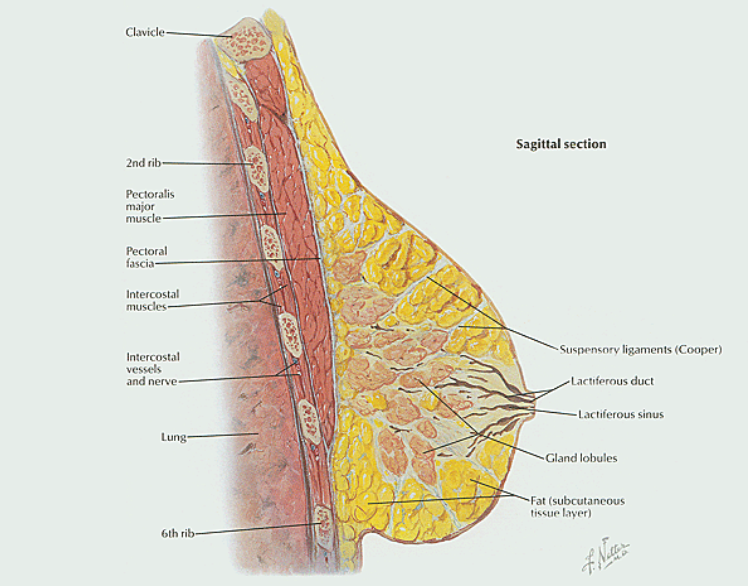
\includegraphics[width=0.8\textwidth]{breast_anat}
    \caption[Breast Structure]{Breast's Structure \cite{Witmer2004}}
    \label{fig:breast structure}
\end{center}
\end{figure}

\section{Breast Cancer and Incidence} \label{sec:incidence}

Breast cancer is caused by the presence of a malignant tumor, known as carcinoma, developed from the breast cells. Despite of being more common in women (99\%), this disease can also affect men (1\%). Portugal follows the same trend as developed countries regarding the diagnosed cases of breast cancer per years. \footnote{\url{http://www.who.int/cancer/country-profiles/prt_en.pdf?ua=1}}

The tumor, regarding its location, can be associated with one or more of the following 6 regions of the breast: upper-inner, upper-outer, lower-inner, lower-outer, nipple and areola complex or axillary tail. Usually the axillary tail is also considered as upper-outer region. Figure \ref{fig:breast regions} shows the breast regions division into quadrants and the nipple and areola complex.

\begin{figure}[H]
\begin{center}
	\leavevmode
    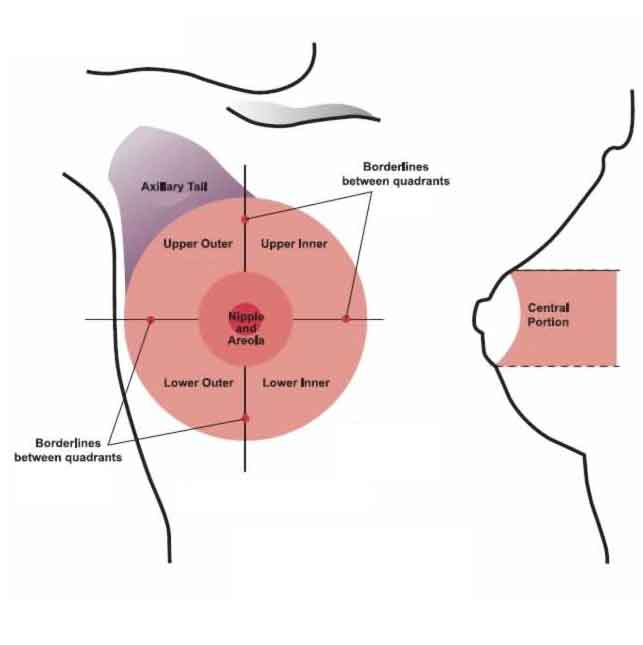
\includegraphics[width=0.5\textwidth]{breast_regions}
    \caption[Breast Regions]{Breast regions \protect\footnotemark}
    \label{fig:breast regions}
\end{center}
\end{figure}
\footnotetext{\url{https://www.pinterest.pt/pin/302304193710434456/}}

According to the study in \cite{Sohn2008}, 57\% of the breast cancer occurs in the upper-outer quadrant, 14\% in the upper-inner quadrant, 10\% in the lower-outer quadrant and 9\% in both the lower-inner quadrant 
and the nipple and areolar complex. The remaining 1\% occur in the axilliary tail.


With the increased concerned regarding cancer diseases, it has been made an effort to diagnose them as soon as possible. In the specific case of breast cancer, as shown in Figure~\ref{fig:breast_cancer_statistics}, 85\% of the patients who are diagnosed in early stages \footnote{ \url{http://www.cancerresearchuk.org/health-professional/cancer-statistics}} are granted a 90\% chance for the cancer be fully cured and provided with a survival rate greater than 88\%. All the diagnosed patients with stage I, II or part of stage III are considered early stages \footnote{\url{https://www.womenshealth.gov/publications/our-publications/fact-sheet/early-stage-breast-cancer.html}}. Early cancer diagnosing allows the patient not only to take less invasive treatments, but also have better aesthetic outcome at the end of treatment.

\begin{figure}[H]
\begin{center}
    \leavevmode
    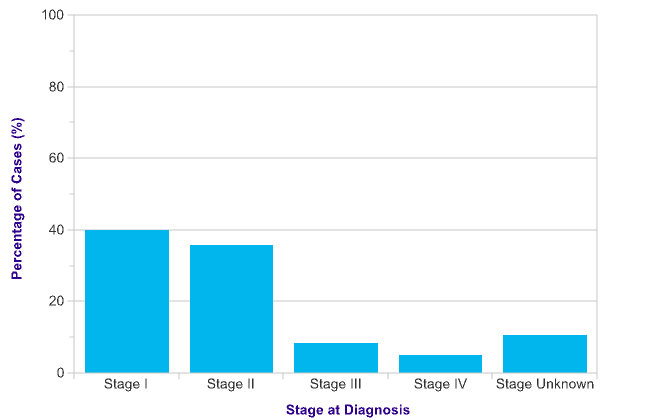
\includegraphics[width=0.85\textwidth]{inc_stage_breast_0}
    \caption[Breast cancer incidence by stage]{Breast cancer incidence by stage \protect\footnotemark}
    \label{fig:breast_cancer_statistics}
  \end{center}
\end{figure}
\footnotetext{\url{http://www.cancerresearchuk.org/health-professional/cancer-statistics/statistics-by-cancer-type/breast-cancer}}

Breast cancer is either considered as both invasive and non-invasive cancer as for spreading to surrounding tissues. The most common example of non-invasive breast cancer is known as Ductal Carcinoma in Situ (DCIS), in this case, the cancer is located on the place where the carcinoma occurred, growing through the milk ducts. If detected in early stages, this type of cancer can be easily cured with a great rate of success, otherwise it can evolve into an invasive breast cancer. On invasive breast cancer, the tumor spreads from the milk ducts and lobules to neighbor tissues. It can be classified in two different types of invasive breast cancer: Invasive Ductal Carcinoma, when the tumor has origin on the milk ducts; or Invasive Lobular Carcinoma, when the tumor has origin on the lobules.

The breast cancer can also be classified in different stages according with the size of the tumor and the affecting tissue.
The Stage 0, refers to the DCIS, with a few abnormal cells in lining of the ducts or small portions of the breast, and as a survival rate near 100\%;
The Stage 1, refers to breast cancer caused by carcinoma with less than 1 inch across (98\% survival rate); 
The Stage 2, refers to breast cancer caused by carcinoma with less than 2 inches across that can spread to some auxiliary lymph nodes  (88\% survival rate);
The Stage 3, refers to breast cancer caused by carcinoma larger than 2 inches across with an extensive spread to auxiliary or nearby lymph nodes. At this stage, some dimpling, inflammation or change of the color skin can be observed (52\% survival rate);
The Stage 4, refers to breast cancer caused by carcinoma spread from the breast to other regions and organs (16\% survival rate); \footnote{\url{http://johnstonhealth.org/2012/10/breast-cancer-awareness/}}

One of the most used and successful ways to diagnose breast cancer is thourgh MRI \footnote{\url{https://radiopaedia.org/articles/breast-mri}}; Mammograms also have an important role evaluating the risk for breast cancer growth, since the medical community has found breast tissue density an important factor for the growth of breast cancer \cite{Saidin2012}. Despite of the large number of breast density classifications, a fluently used is the Breast imaging-reporting and Data system (BIRADS) developed by the American College of Radiology (ACR) \cite{Saidin2012}.

The 4 categories defining the breast's density are enumerated below: \footnote{\url{https://radiopaedia.org/articles/breast-density}}
\begin{itemize}
\item \textbf{1} - fatty: breast is almost entirely fat;
\item \textbf{2} - scattered fibroglandular: breast has scattered areas of fibroglandular density;
\item \textbf{3} - heterogeneously dense: breast tissue is heterogeneously dense;
\item \textbf{4} - dense: breast tissue is extremely dense.
\end{itemize}

\section{Breast Cancer Treatment}\label{sec:treatment}

The goal of breast cancer treatment on early stages of the disease is to completely remove the cancer and preventing its recurrence. On later and more advanced stages of the cancer, it cannot be cured, so, the treatment techniques on this scenario focus on the attenuation of its effects and symptoms together with improving the QoL of the patient.

For years, the mastectomy has been the answer to treat breast cancer. Nowadays there are treatments with better results in terms of tumor removal and with a minor influence on the patients QoL, replacing the mastectomy by treatments such as BCS and oncoplastic treatments.

On the case of breast cancer on men, the mastectomy is always the recommended treatment option. However, for women, there are a lot of different treatment options that can vary between surgery to several therapies and a combination of them.

The treatments can be classified as local treatments or systemic treatments. The local treatments are applied on early cancer stages, treating tumors without affecting other parts of the body. When the cancer has already spread to surrounding tissues, systemic treatments are preferred in order to treat tumor cells on different areas of the patient's body. Some of the examples of local treatment are surgery and radiotherapy, while systemic treatments are composed by chemotherapy, hormone therapy or targeted therapy. This types of treatments may be combined to reach better results leading to two different types of therapy: neoadjuvant therapies and adjuvant therapies, that combine local and systemic treatments in order to treat a patient. The neoadjuvant therapy consists on applying systemic treatments before the surgery to reduce the carcinoma size. This allows to remove a smaller portion of the tumor during surgery and can be applied on cases that were considered inoperable due to the increased tumor size. The adjuvant therapy consists on complementary treatments applied after the surgery in order to eliminate cancer cells that may have spread previously to the surgery or eliminate cells not removed during the surgery \cite{De2016}.

As mentioned before, surgery is the most frequent option to treat breast cancer. However, it may be done for other reasons either than removing the tumor and the surrounding tissue, listed below:

\begin{itemize}
\item Perform biopsies on sentinel lymph nodes, in order to find if the cancer cells had spread to the axillary lymph nodes.
\item Breast reconstruction, to restore the breast shape after removing the tumor
\item Relieve symptoms of advanced breast cancer.
\end{itemize}

The most common types of surgery are Mastectomy and Breast Conserving Surgery, represented in Figure~\ref{fig:Breast Cancer Surgery}. Both are performed in order to remove the tumor and the surrounding tissue on the patient's breast.

\begin{figure}[H]
    \centering
    \subfloat[Mastectomy]{{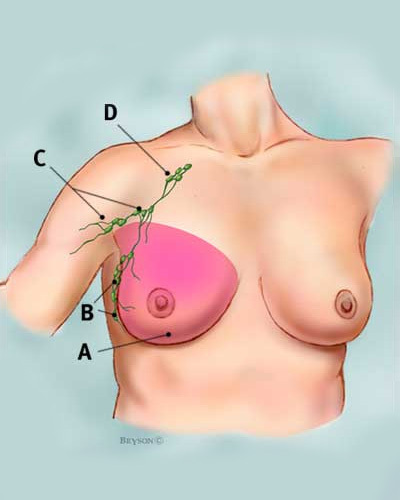
\includegraphics[width=5cm]{mastectomy} }}
    \qquad \qquad \qquad
    \subfloat[Breast Conserving Surgery]{{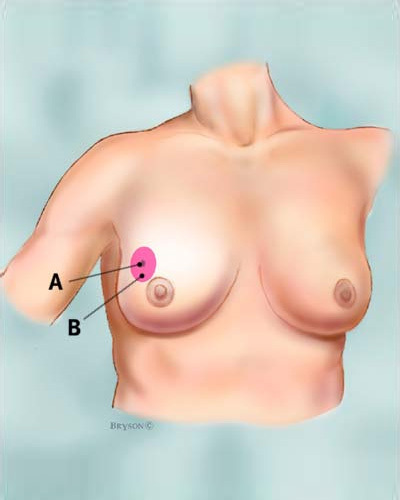
\includegraphics[width=5cm]{lumpectomy} }}
    \caption[Breast Cancer Surgery]{Breast Cancer Surgery \protect\footnotemark}
    \label{fig:Breast Cancer Surgery}
\end{figure}
\footnotetext{ \url{http://www.breastcancer.org/treatment/surgery}}

\begin{itemize}
\item \textbf{Mastectomy}

Even though the different approaches within the Mastectomy: radical mastectomy, modified radial mastectomy, simple mastectomy and skin-sparing mastectomy, all the above consists on the extraction of the entire breast tissues and some of the surrounding tissues. In the case of radical mastectomy, the pectoral muscle and all the axillary lymph nodes are also removed. Despite of the remotion of a great volume, the mastectomy do not remove tissues beyond the clavicle, the inframammary fold (above the rectus sheath), the midline of the sternum and the anterior border of the latissimus dorsi \cite{Witmer2004}. Less radical surgeries have been proved as effective as this. Nowadays, mastectomy is only performed for patients with large tumors that have spread into the pectoral muscle.

\item \textbf{Breast Conserving Surgery}

Breast Conserving Surgery (BCS), as known as partial mastectomy or lumpectomy, is a less extreme way to surgically remove the tumor. This procedure aims to remove the least possible amount of breast tissue, containing only the tumor and a small portion of the healthy tissue surrounding it. BCS is much less invasive than Mastectomy and with the same effectiveness and survival rates when radiotherapy is used as complementary treatment. Even though some women prefer the mastectomy, fearing the recurrence of the cancer, studies have proven that mastectomy do not provide any better result regarding the cancer treatment and recurrence than BCS, and the number of patients choosing this option as treatment has increased.
\end{itemize}

\section{Impact of Breast Cancer Treatment}

\subsection{Influence on the Aesthetic Outcome}

Several studies have been made in order to understand what parameters and how they influence the aesthetic outcome of BCS. These studies have evaluated parameters such as the age of the patient, her body mass index, the existence of palpable tumors, the location, volume and weight of the tumor, the axillary and breast incisions during surgery, among other factors.

It is also known that radiotherapy and chemotherapy have influence on the aesthetic result; however, all the studies regarding the adjuvant therapies influence are merely based on empirical experiences on patients.

According to \citet{Foersterling2014} previous studies have concluded that, generally, when the tumor is located on the inner quadrants of the breast, the treatment results in a poor aesthetic outcome. The location of the tumor on the nipple areolar complex leads to the most unfavorable aesthetic outcome. Unlike the location, the tumor weight has not been proved as predictive of a bad aesthetic outcome, in spite of tumors with less than 50g tend to lead to good aesthetic outcomes according with the aesthetic evaluation metrics presented in \cite{Joa2012}.

Concerning, the breast incision and besides of the inconsistent findings, some authors associate better aesthetic outcomes with radial and circular incisions, and worst outcomes with the periareolar one \cite{Foersterling2014}. Other studies point aspects like the result of mechanical forces such as gravity, breast tissue constitutive law distribution, inflammation due radiotherapy, the internal stress generated by the healing process and angiogenesis as factors on the breast shape after Breast Conserving techniques \cite{Vavourakis2016}. The aspect of the breast may change significantly during the healing process that can take as long as two years due to alteration regarding the tissue composition, stiffness and volume.

\subsection{Quality of Life}

Changes of the breast's size or shape or even the loss of it have a significant impact on the psychological and social life of a patient. The loss of breast as a symbol of femininity has may lead to a decrease of the patient's self-esteem, negative body image, social isolation and communication and relationship problems. The psychosocial stress and the physical burden may result in a reduction of the patient's opportunities in life and increase their social rejection. Common symptoms of the breast cancer treatment visible on a wide number of patients are anxiety, depression, fatigue, pain, difficult in concentration, sexuality concerns and self-blame \cite{Al-Azri2014}. Despite of the sparsity of studies regarding the influence of breast treatment surgeries on women's body image and sexuality, the most recent ones consider BCS result on a best preservation of the woman's body image and more comfort about their sexuality \cite{Rowland2000}.

\section{Summary}

Given the importance of the visualization of a treatment outcome on a breast cancer treatment and the impact it has on the QoL of the patient, the ability of predicting the aesthetic outcome of a surgery is a valuable aspect.

Currently, this is shown with 2D drawings and pictures of similar cases, and in some cases with generic 3D models. A patient-specific prediction will allow to minimize the doctor-patient misunderstandings, to find the optimal treatment, to decrease the fear the patients stood against surgery and to select the most desired outcome of the surgery. In order to achieve this, it is important to be able to manipulate a 3D breast model, and define the transformations that each treatment may led on the patient's breast. As outcome, the patient may be able to see own breast deformed in a real time system.

The next chapter describes the models that are being used so far and how a breast model may be represented as well as some existing simulations of the breast surgery.

\chapter{3D Modeling of the breast}\label{chap:modeling}

\section*{}

In order to achieve a prediction of the aesthetic outcome after a BCS the best option is to describe the breast using 3D models. Some models can be reached with several techniques, but all of them retrieve a model with some compression or mechanical force present.

Due to the importance on medical imaging to find a smooth surface that fits a set of 3D unstructured data to describe and represent anatomical structures, many alternatives have been found over the years. Being a complicated problem and due to the variability and difference between the shape of human breasts, a lack of work on this field was led to \cite{De2016}.

The present chapter starts by presenting several data acquisition techniques, in section \ref{sec:acquisition}, that could provide the information for generating 3D models. The data may be represented using for example parametric and deformable models presented in section \ref{sec:param} and section \ref{sec:deform}, respectively. At the end of the chapter some existing frameworks used for breast augmentation and plastic surgery are referred in section \ref{sec:ferramentas}, such as the methods that they use in order to acquire and model 3D data.


\section{Data Acquisition}\label{sec:acquisition}

Despite of all the several ways to describe and represent the shape of breast, the 3D imaging yields more information than multiple conventional photographs. Given this, 3D models are the best and more realistic way to evaluate the shape and size of the breast, its symmetry, contour, volume and surface area \cite{Kim2008}.

Multiple attempts have been done to represent breast as a 3D object. Those attempts have started by using Magnetic Resonance Imaging (MRI), Computed Tomography (CT) and 3D surface imaging systems. Bücking et al. in \citep{3dprintplos} describes the use of CT and MRI data to generate 3D models of anatomical human parts in order to 3D print the obtained models. In this case a pre-processing of the data was done considering two main steps: image segmentation, where the image was labelled and partitioned into several areas and regions ignoring the noisy regions of the image; and a mesh refinement, repairing and smoothing the models' discontinuities. The authors also mentioned that CT was used instead, when segmenting structures with low or high densities. MRI are best used in soft tissues due the high contrast on this cases.

An alternative to retrieve 3D models of the patient's torso was proposed in \cite{Costa2014}. This approach used a low-cost depth sensor (Microsoft Kinect) to acquire several views of patient's torso in order to perform a point cloud registration of the breast. The point cloud registration process is subdivided into two parts: coarse registration and fine registration. In order to generate the point cloud that would serve as input in the coarse registration, the raw RGB-D data acquired by the sensor were pre-processed. The pre-processing started by segmenting and then filtering the depth image in order to remove the noise on the edge and silhouette of the object. Given the retrieve point could, a Tessellation-based coarse registration uses depth data to align the point clouds. The alignment was done by a pose estimation, to reduce the initial misalignments; a keypoint selection to identify some correspondences between different point clouds; and a correspondence estimation and validation to find the better coarse alignment.

According to \citet{apenn}, the acquisition of MRI data consist of several MRI axial slices of the breast and ensures the 3D visualization of the patient's breast. In the cases where the acquisition of MR images is not axial, it can be converted posteriorly. Thereafter and despite of the semi-automatic segmention of the MRI data contours, the images required a manual segmentation in order to differ parenchyma, fat and lesion tissues. Based on the segmentation results and the defined contours it is possible to calculate a few reference points and then generate a 3D computational mesh. The generated mesh is represented by parallel planes limiting the breast's contour.

\section{Parametric Models}\label{sec:param}

Once the raw 3D data are obtained and due to the need to easily manipulate it, depending on its application, the information acquired may need to be represented or transformed in any other type of 3D representation. In the case of medical application such as representing human organs, the parametric models are widely used. An application of parametric models was described in \cite{Vision1998} when representing the left ventricle of the heart. These models have as advantage using superquadrics parameters allowing to represent objects with rounded edges or corners that may resemble a wide variety of human organs. 

The fitting of superquadrics to 3D unstructured data being a problem, it was already investigated, what led to some robust and fast methods that solved it. A superquadric refers to different sets of superellipsoids, supertoroids or even one or two pieces of superhyperboloids. And despite of the general use of superellipsoids, presented in Figure \ref{fig:superellipsoids} the other objects can also be used in order to describe different shapes.

\begin{figure}[H]
\begin{center}
    \leavevmode
    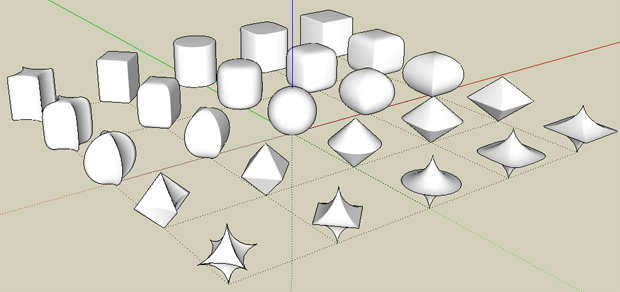
\includegraphics[width=0.85\textwidth]{superellipsoid}
    \caption[Examples of superellipsoids]{Examples of superellipsoids \protect\footnotemark}
    \label{fig:superellipsoids}
  \end{center}
\end{figure}
\footnotetext{\url{http://regular-polygon.com/plugins/superellipsoid/}}

A superquadric is obtained by the spherical product of two 2D curves. In the case of a superellipsoid, it is described by the following equations.

\begin{equation}
\left ( \left ( \left ( \frac{x}{a_1} \right )^{\frac{2}{\varepsilon_2}} + \left ( \frac{y}{a_2} \right )^\frac{2}{\varepsilon_2} \right )^\frac{\varepsilon_2}{\varepsilon_1} + \left ( \frac{z}{a_3} \right ) ^\frac{2}{\varepsilon_1} \right ) ^ \frac{\varepsilon_1}{2} = 1
\end{equation}

The parameters $a_1$, $a_2$ and $a_3$ are scaling factors corresponding to the coordinate axis, and $\epsilon_1$ and $\epsilon_2$ represent the squareness of the original superellipsoids.

A smaller $\epsilon$ represents a superellipsoid similar to a square, $\epsilon$ equal to 1 represents a circle and $\epsilon$ equal to 2, a shape with a flat bevel and a superellipsoid with larger $\epsilon$ defines a pinched shape.

In order to pose the superquadric on an axis system, 6 more parameters are required.

\begin{equation}
Xw=T.Xs, T= 
\begin{bmatrix}
R&t\\
0&1\\
\end{bmatrix}
\end{equation}

R is a 3x3 matrix and t a 3x1 matrix representing the rotation and translation, in relation to the referrals' origin, of the superquadric respectively.

As soon as the most adequate superquadric is chosen, it must fit the 3D data that we want to represent. Despite of the good global approximation of a shape, superquadrics are too limited when representing more complicated surfaces. This problem usually occurs due to the symmetry of the superquadrics. A possibility to overcome is the utilize deformable models presented on section \ref{sec:deform} or its application of the parametric models refereed in \cite{Pernes2014}.



\section{Deformable Models}\label{sec:deform}
Representing the 3D data of the patient's breast using Deformable models will allow generating and manipulating complicated curves and surfaces. The deformations that would be applied in order to generate that kind of complex data can be categorized in two different methods Physical Methods and Non-Physical Methods. While the Non-Physical Methods manually manipulate and deform the objects by adjusting one or more parameters of the shape (that describe the more simple object), the Physical Method relies on the modification of the physical properties of the object through the application of external forces. In the case of Physical methods, the material's properties of the object also impact the deformation of the object \cite{Gibson97asurvey, De2016}.


\subsection{Non-Physical Models}

As mentioned before, the non-physical methods to deform object are done recurring to the alteration of model parameters. Widely used ways to represent curves defined by vectors of control point vary between Bezier curves, B-splines or non-uniform rational B-splines (NURBS).

The abovementioned approach in \cite{Pernes2014} and \cite{Vision1998} is based on the application of Free Form Deformation (FFD). The FFD allows to define the deformations by adjusting the space where the object lies and not by changing its control points. Another advantage of this approach is that the same deformation can be applied to the different models simultaneously.

On this specific approach the model is considered to be embedded in a box that can be changed in order to twist, bend or taper the model on its interior. Figure \ref{fig:FFD} shows the object embedded on the box of control points in \ref{fig:FFD_BB} and the result of the object deformation in \ref{fig:FFD_applied}. To accomplish this, the FFD formulation shall be done in the two following steps:

\begin{enumerate}
\item Compute the local coordinates of the object points in the frame defined by the box of control points.

\begin{equation}
X = X_{0} + s S + t T + u U,
\end{equation}

where \textit{s}, \textit{t} and \textit{u} are given by:

\begin{equation}
s = \frac{S. \left(X-X_{0} \right)}{S.S},   t = \frac{T. \left(X-X_{0} \right)}{T.T},   u = \frac{U. \left(X-X_{0} \right)}{U.U}, 
\end{equation}

\textit{X} represent each point of the objects by the coordinates (\textit{s},\textit{t},\textit{u}) and the box where the object is embedded is represented by the vertex \textit{$X_{0}$} and the box edges (\textit{S},\textit{T},\textit{U}).

The point \textit{X} is inside of the box if and only if \textit{s}, \textit{t} and \textit{u} have all values between 0 and 1.

The size of the embedding box is given by the parameters $a_{1}$, $a_{2}$ and $a_{3}$ of the superquadric and its rotation is given by the coefficients of the rigid transform $\varphi$, $\theta$, $\psi$, $t_{x}$, $t_{y}$ and $t_{z}$.

The volumetric grid of the box's control points $\left( l+1 \right)$ $\left( m+1 \right)$ $\left( n+1 \right)$ can be described by:

\begin{equation}
  \begin{cases}
  	x(\textbf{$P_{ijk}$}) = a_{1} \left(1-2 \frac{i}{l} \right) \\
  	y(\textbf{$P_{ijk}$}) = a_{2} \left(-1+2 \frac{j}{m} \right) \\
  	z(\textbf{$P_{ijk}$}) = a_{3} \left(1-2 \frac{k}{n} \right) 
  \end{cases}
\end{equation}

At last, the space alterations that the model will be put through may be represented as:

\begin{equation}
X = BP,
\end{equation}

where \textit{X} is a matrix NP x 3 (NP: number of control points = (l+1)(m+1)(n+1)) with the coordinates of the model points, \textit{B} is the deformation matrix ND x NP (ND: number of points on the object) and \textit{P} the NP x 3 matrix which contains coordinates of the control points $P_{ijk}$.

\item To achieve the best fitting of the model to the data we intent to represent, the displacement field must be reduced. This displacement refers to the distance between the model and the data points we will represent.

We are changing position of control points to fit X to the target model. Note that we are not fitting control points to sth.

As soon as the best fitting of the model is find, by changing the position of control points in order to make \textit{X} fit the target model, the position of point \textit{X} of the object may be computed.

\end{enumerate}

\begin{figure}[H]
\begin{tabular}{ll}
\subfloat[Box of control points with embedded object]{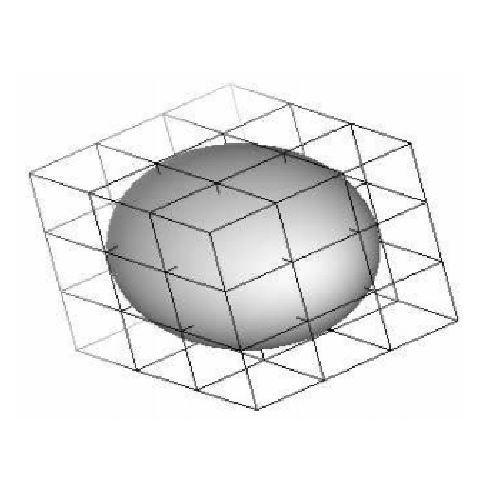
\includegraphics[width = 3in]{FFD_BB}\label{fig:FFD_BB}} &
\subfloat[Object of the deformed box]{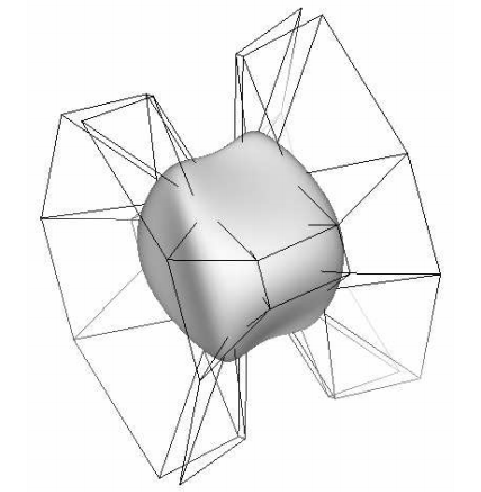
\includegraphics[width = 3in]{FFD_applied}\label{fig:FFD_applied}}
\end{tabular}
\caption[FFD deformation]{FFD deformation \cite{Vision1998}}
\label{fig:FFD}
\end{figure}

\subsection{Physical Models}
A well-studied physical model is mass-spring method which is used in modeling facial expressions. The proposed methodology described in \cite{Gibson97asurvey} uses three distinct layers of tissue in order to deliver a mesh of mass points corresponding to the dermis, a layer of fatty tissue and a layer of muscular tissue. The same approach has been adopted in the context of breast surgery \cite{1085f1d}, where a volumetric tetrahedral mesh representing the breast was computed from a semi-automatic segmentation procedure. Then the mesh was deformed based on the mass-spring model: the spring's rest length and stiffness were estimated and then applied to the uncompressed breast model in order to deform it to the real compressed one. Although being easy to construct and allow to deform the objects in more ways than other physical methods, mass-spring finds difficult to model incompressible volumetric objects or unbendable surfaces.

Another method with a great variety of applications is Finite Element Models (FEM). In contrast with the mass-spring method, FEM is more accurate, requiring a much larger computational power and being a very time consumption process. In a FEM, the object is divided into several elements joined by discrete node points. The desired deformation function is then applied to each element in order to find an approximation that satisfies an equilibrium expression relative to the intended deformation. The type of elements that are used to form the model are chosen according to the properties of the object, the trade-off between the computational power and the required accuracy. One of many examples of the application of FEM was described in \cite{Kurihara2004} where simullating the interacting between the soft tissue of a human hand and a deformable object. Considering the apllication of FEM in breast surgery, it has been used in \cite{Vavourakis2016}, whose proposed methodology will be further detailed.

\vspace{12mm}

Vavourakis et al. \cite{Vavourakis2016} proposed a surgical simulator based on a FEM. In order to simulate the wound healing effect described in \cite{Vavourakis2016} data was gathered though MRI as described in \cite{apenn}. The used mesh is constituted by two distinct types of isoparametric elements, shown on Figure \ref{fig:3d_mesh}:

\begin{itemize}
\item Solid 4-node trilinear isoparametric elements - used to represent the breast tissues except for the skin;
\item 3-node triangular isoparametric elements - used to represent the surface of the model: the breast's skin.
\end{itemize}

\begin{figure}[H]
\begin{center}
    \leavevmode
    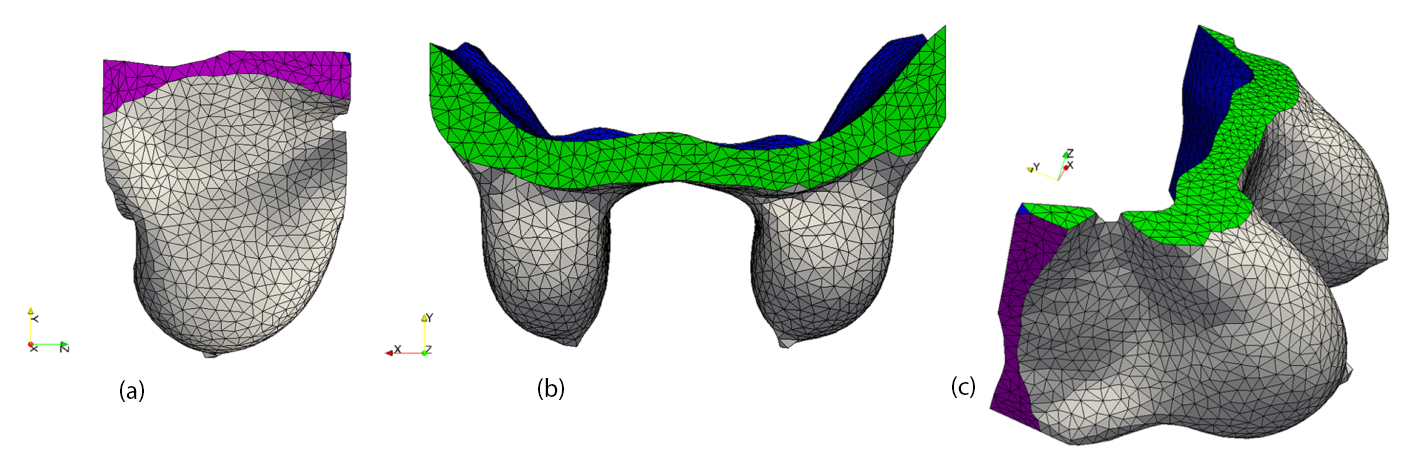
\includegraphics[width=0.85\textwidth]{FE}
    \caption[3D mesh with isoparametric elements]{\textbf{3D mesh with isoparametric elements} (A) Lateral View (B) Caudal View (C) 3D View \cite{Vavourakis2016}}
    \label{fig:3d_mesh}
  \end{center}
\end{figure}

In the obtained 3D mesh, a material is assigned to the elements that represents it on the mesh. This assignment is based on the different types of tissue: fat, parenchyma and damaged. Each type of tissue on the mesh will be assigned it a different type of materials.

Vavourakis et al. \cite{Vavourakis2016} described the implementation of a surgical simulator based on Multiscale FEM, where two concurrent simulations were performed: a wound healing simulation and a biomechanical simulation. This implementation is represented in Figure \ref{fig:surgical_simulator}, whose steps are described below:

\begin{figure}[H]
\begin{center}
    \leavevmode
    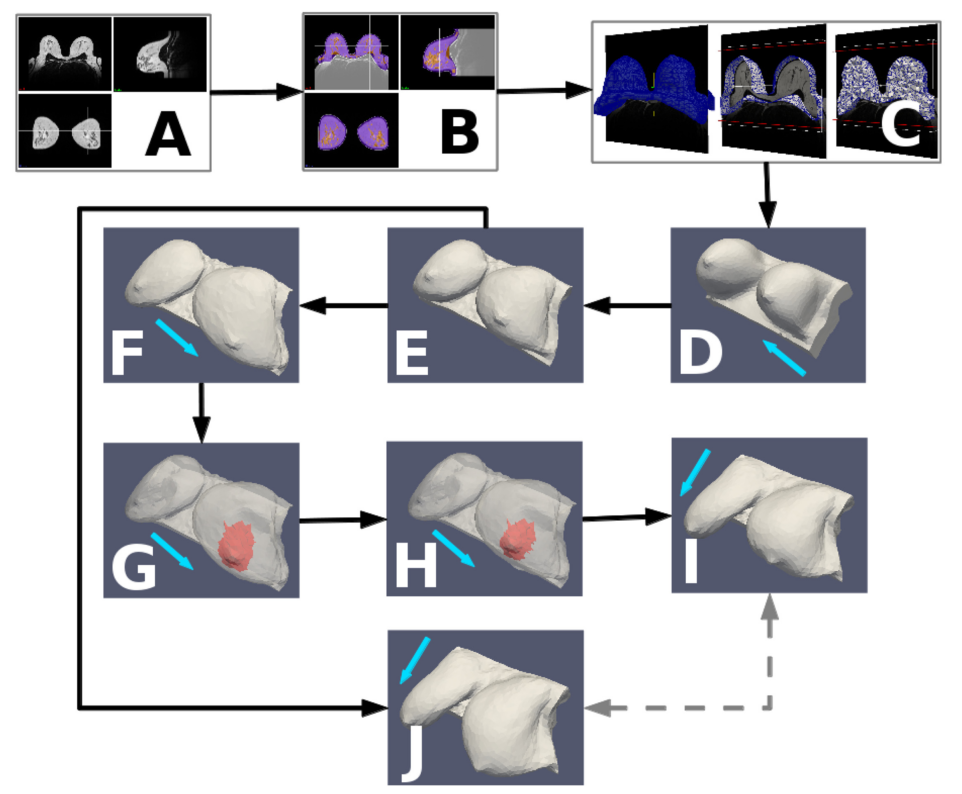
\includegraphics[width=0.85\textwidth]{oneplus}
    \caption[Example of computational process for surgical simulator]{Example of computational process for surgical simulator \cite{Vavourakis2016}}
    \label{fig:surgical_simulator}
  \end{center}
\end{figure}

\vspace{24mm}

\begin{itemize}
\item In step A, the MRI data and the computed-tomography (CT) data are acquired;
\item In step B, the data is segmented, differing the adipose and fibroglandular tissues of the breast;
\item In step C, the generation of the surface and volumetric meshes of the patient's breast is possible through the data acquisition and segmentation referred in the previous steps;
\item In step D, the models are prepared for the input of the Finite Element solver;
\item The retrieved data from MRI are represented in prone since they are stressed by the gravity force. In order to apply mechanical finite element models, the step E is required to remove the gravity effect on the model, computing the a gravity unloaded model;
\item In step F, the gravity unloaded model of the breast is converted into a supine geometry;
\item In step J, the gravity unloaded model of the breast is also used to predict the breast's geometry in upright;
\item In step G, the tumor position is identified through determining the incision lines and the outline of the excised tissue. Consequently, the elements inside the outline of excised tissue are labeled as damaged tissue;
\item Step H, performs the wound healing simulation resulting in the wound contraction and the estimation of the post-surgery breast shape;
\item Finally in step I, the effect of gravity is re-applied on the breast shape, retrieving the model in a stand up position, or upright geometry.
\end{itemize}

\vspace{12mm}

The proposed surgical simulator that estimates the wound healing and the pos-surgical shape of the breast relies on the two mathematical models described below:

\begin{itemize}
\item Wound Healing and Angiogenesis Model

This mathematical models is based on the cell density, the concentration of biochemical agents responsible for the mitosis regulation, the density of the microvascular density, the nutrient and oxygen levels and the agent that regulates vascular spouting in order to compute the changes on the breast shape during the healing process. It also takes into consideration the increase of the inflammatory response and the stimulation of the immune system.

\item Soft Tissue Biomechanics Model

Also responsible for the configuration of the breast geometry, the Soft Tissue Biomechanics model takes into account the breast tissue's mass density and the body force vector. Within this model, the stress distribution is calculated considering the passive stress of the tissues' mechanical deformations and the active stress from the tissue recovering during the wound healing process.  

\end{itemize}

\section{Existing Frameworks}\label{sec:ferramentas}

The greater portion on this field focuses on breast augmentation and plastic surgery and have originated some software able to simulate deformations on the breast tissue. Being the most known:

\begin{itemize}
\item Crisalix \footnote{\label{crisalix} \url{https://www.crisalix.com/en}}

Crisalix is a web based application based on 2D photographs with a range of implant types, sizes and surgery techniques available. Figure \ref{fig:crisalix} shows Crisalix software, that allows to simulate breast enlargement or reduction, breast lift, the application of silicone implants, implants revision, scars, breast reconstruction and fat transfer.

\begin{figure}[H]
\begin{center}
    \leavevmode
    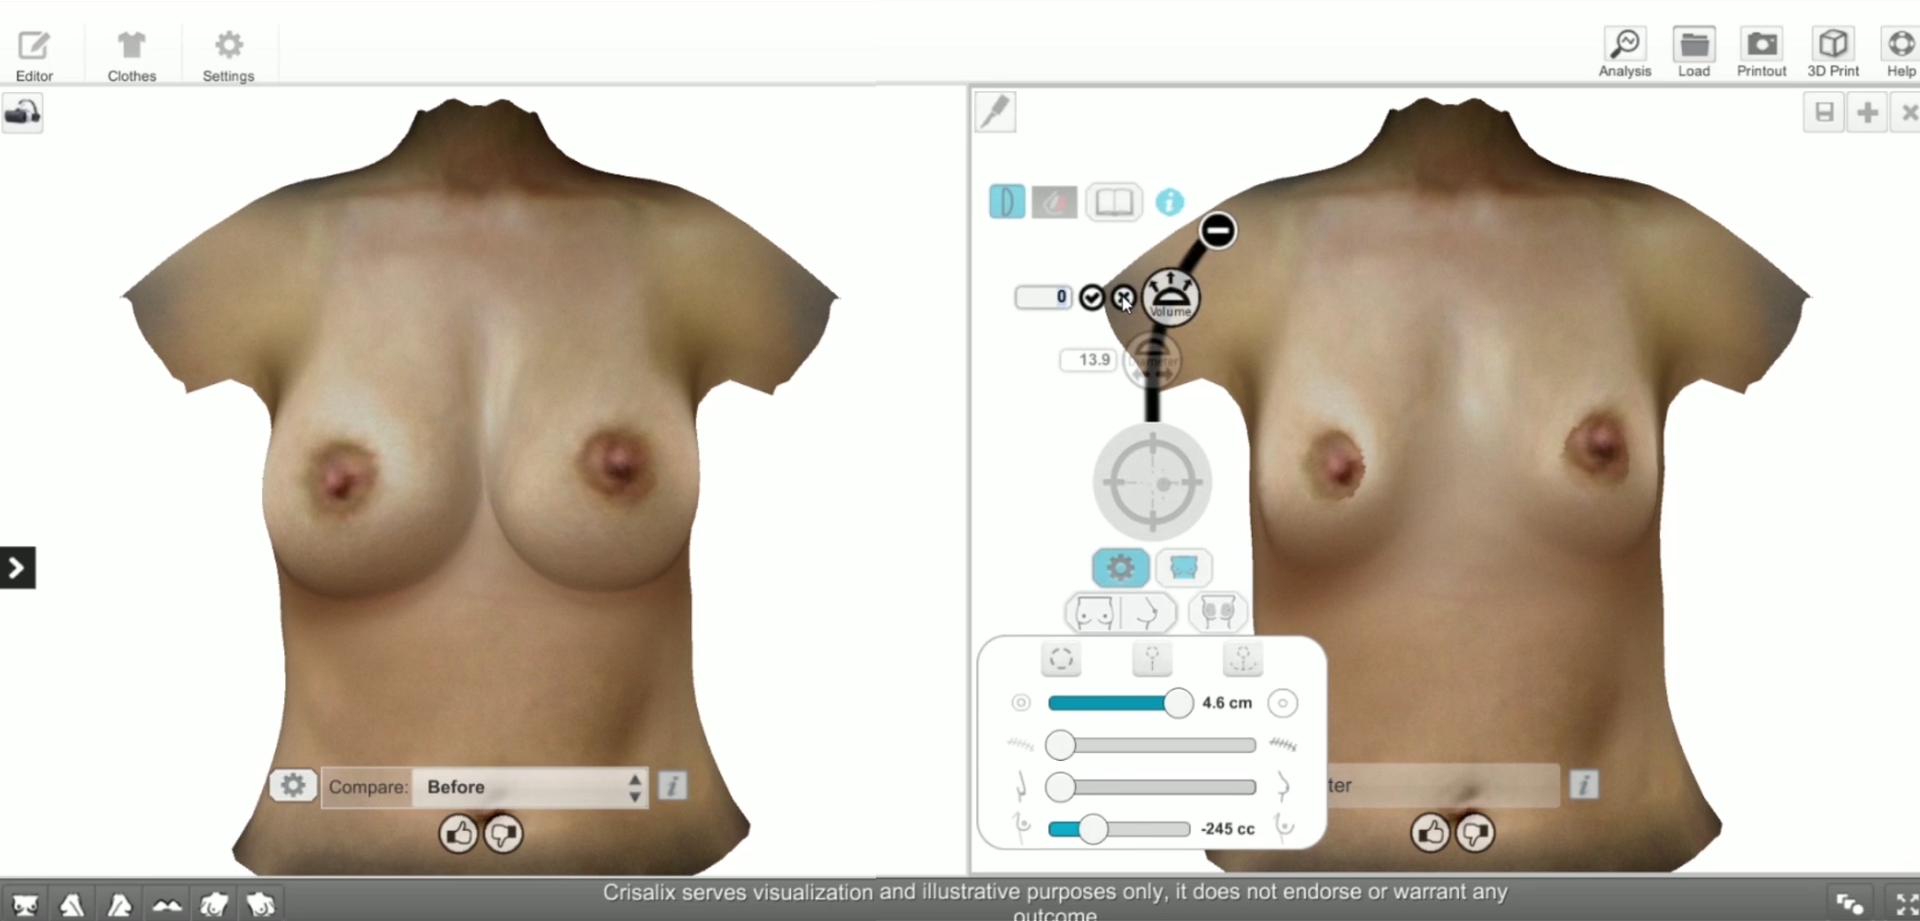
\includegraphics[width=0.5\textwidth]{crisalix}
    \caption[Crisalix interface]{Crisalix interface \textsuperscript{\ref{crisalix}}}
    \label{fig:crisalix}
  \end{center}
\end{figure}


\item Sculpt My Dream \footnote{\label{sculptmydream} \url{http://www.sculptmydream.com/}}

Sculpt My Dream is a property platform of Vectra3D, and uses six distinct cameras to reconstruct a virtual model of the patient's torso. The simulation relays on a variety of implant sizes and a list of manufacturers while is able to correct some asymmetry of the breast. Even though the good estimation and the similarity between the software simulation and the procedure, it can only be applied to plastic surgery. Figure \ref{fig:sculptmydream} shows Sculpt My Dream interface.

\begin{figure}[H]
\begin{center}
    \leavevmode
    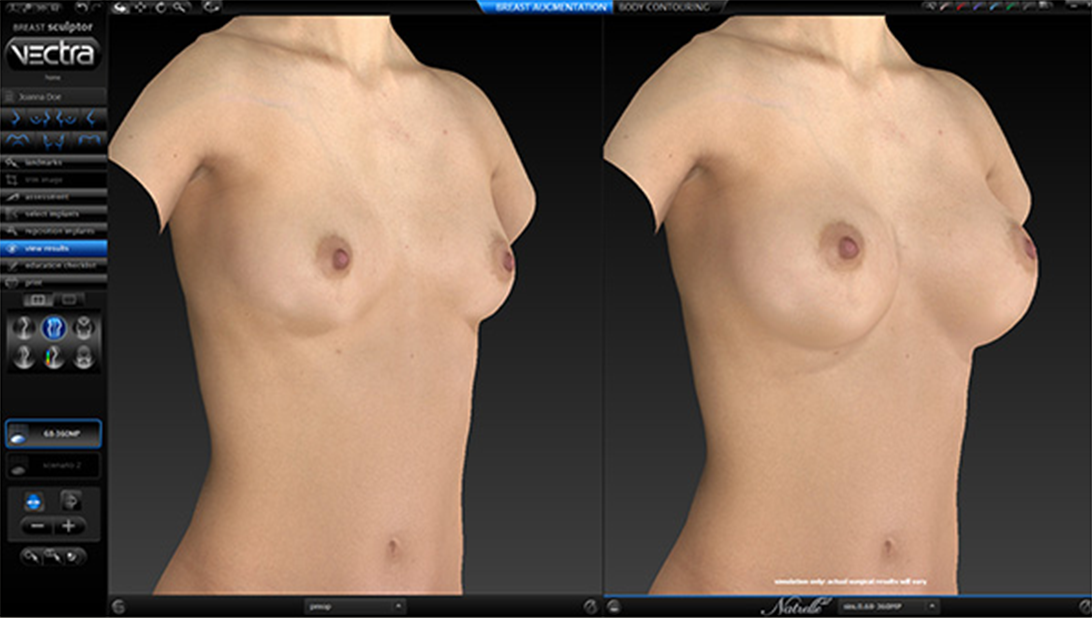
\includegraphics[width=0.45\textwidth]{sculpmydream}
    \caption[SculptMyDream interface]{Sculpt My Dream interface \textsuperscript{\ref{sculptmydream}}}
    \label{fig:sculptmydream}
  \end{center}
\end{figure}

\item Axis Three \footnote{\label{threeaxis} \url{http://www.axisthree.com/welcome}}

Axis Three uses a property scanner to capture 3D images of the patient's torso. It simulates alterations on the face or breast of the patient. In the specific case of breast simulation, it is based on the manufacturers implant, the location of the implant (beneath or above the pectoral muscle) and the tissue's elasticity. Figure \ref{fig:threeaxis} shows Axis Three interface.
 
 \begin{figure}[H]
\begin{center}
    \leavevmode
    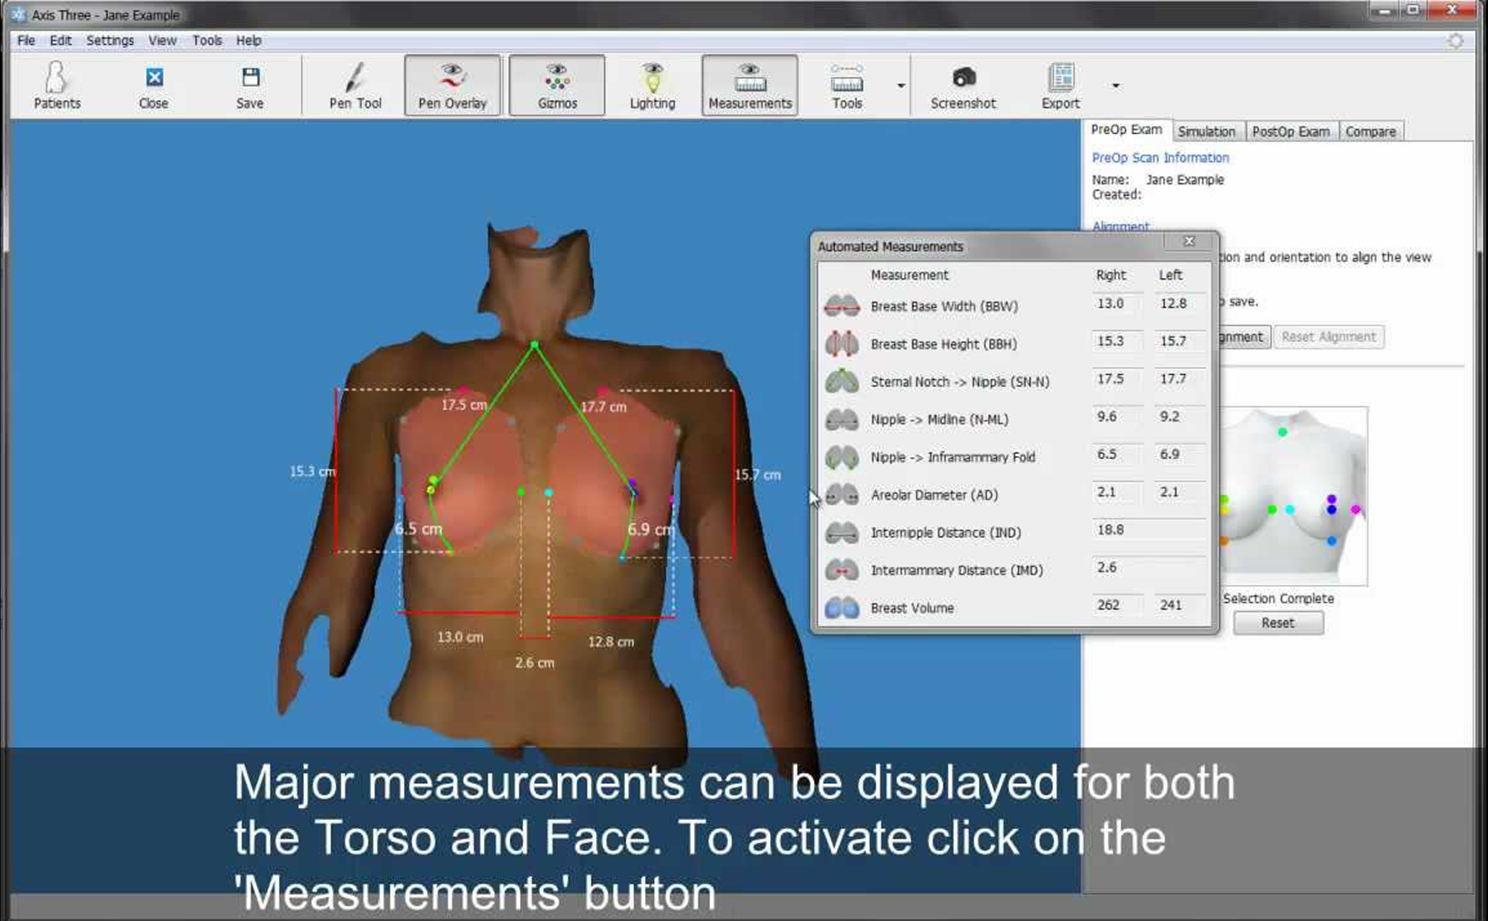
\includegraphics[width=0.45\textwidth]{threeaxis}
    \caption[Axis Three Software]{Axis Three interface \textsuperscript{\ref{threeaxis}}}
    \label{fig:threeaxis}
  \end{center}
\end{figure} 
 
\end{itemize}

In spite of the reliability of these 3D scanner, the utilization of several cameras are demandingly expensive and while it requires complicated procedure to perform 3D reconstruction of the patient's torso.

\section{Summary}

The patient's 3D models, including torso, or individual organs, have been commonly used in applications of both medical tools. In this chapter, a brief descriptions of recent methodologies have been explained as well as their medial applicastions.

Concerning the representation of humans breast, most of the studies focused on the application of the models for plastic surgery. More recently, FFD was used in order to represent the breast's shape; and FEM researched in order to simulate wound healing and transformations between different geometry configurations of the breast.

Despite of the existence of a surgical simulator, time consumption and computational power requirements of FEM makes it unviable to be used in real-time systems. Machine learning techniques will be applied in order to predict the same deformation caused by the BCS in order to overcome the problems of the FEM approach. This methodology is detailed in chapter \ref{chap:method} and its results are presented in chapter \ref{chap:results}.

\chapter{BCS planning tool}\label{chap:tool}

\section*{}

A BCS tool, having as main objective to assist health professionals to understand the surgical outcome, requires the definition of the tumor on the specific breast of the patient. The same tool will also be used to create the dataset as explained in section \ref{sec:dataset_prep}. The tumor location and size will be used to predict the aesthetic outcome of a BCS considering the shape of the patient’s breast and the specific parameters of the tumor, using the obtained prediction models described in chapter \ref{chap:method}.

In this chapter the Functional such as Actors, Functionalities, Use cases and User stories and non Functional requirements of the software are presented, as well as some considerations concerning the interface’s design and the application flow.

\section{Functional Requirements}

The Functional requirements describes the system and its functionalities and components such as the actors and the way they interact with the system.

\subsection{Actors}

\subsubsection{Health Professional}

Both surgeons and radiologists are considered as health professional and are allowed to perform any of the functionalities presented on the tool.

\subsection{Functionalities}

The developed tool consists of the following functionalities:

\begin{itemize}
\item Loading Breast Model
\item Exporting Tumor and Excision Information, considering the breast's density
\item Visualizing model:
\begin{itemize}
\item Zoom model
\item Change model Point Size
\item Orthogonal views
\end{itemize}
\item Locating nipple
\item Breast Division:
\begin{itemize}
\item Show / hide breast's quadrants
\end{itemize}
\item Defining tumor :
\begin{itemize}
\item Tumor position, by either selecting a point or randomly choosing a position within the defined region  
\item Tumor size
\end{itemize}
\item Defining excision:
\begin{itemize}
\item Excision radius
\end{itemize}
\item Visualizing information:
\begin{itemize}
\item Tumor position - quadrant
\item Breast's Laterality
\item Breast's Volume
\item Tumor radius
\item Tumor volume
\item Excision Volume
\item Excision / Breast volume ratio
\end{itemize}
\item Undo
\item Redo
\item Reset
\end{itemize}

These functionalities will be further detailed on the use cases diagram and the user stories table.


\subsection{User Stories}

The system's user stories are described in Table \ref{tab:user stories}.

\begin{longtable}{|l|p{30mm}|l|p{90mm}|}
%\label{label}\\
\caption{User Stories of BCCT planning tool}\label{tab:user stories}\\
\hline
\textbf{ID} & \textbf{Name} & \textbf{Priority} & \textbf{Description} \\
\hline
\hline
\endhead
\hline
\endfoot
US001       & Load Model             & High                 & As a User, I want to load a specific breast's model of a patient.                    \\ \hline
US002       & Model Visualization             & High                 & As a User, I want to rotate, zoom or pan the loaded model for visualization.                   \\ \hline
US003       & Change orthogonal View             & High                 & As a User, I want to visualize the breast model on an orthogonal view (front, top, bottom, back, lateral).                    \\ \hline
US004       & Define Nipple Position             & High                 & As a User, I want to be able to define the nipple position on the point cloud.                   \\ \hline
US005       & Breast division             & Medium                 & As a User, I want to show or hide the breast quadrants (Upper Outer, Upper Inner, Lower Outer, Lower Inner).                    \\ \hline
US006       & Zoom in / Zoom out             & Medium                 & As a User, I want to Zoom in or Zoom out the breast's model.                   \\ \hline
US007       & Change point size             & Medium                 & As a User, I want to Increase or Decrease the point cloud's point size.                   \\ \hline
US008       & Define the tumor position             & High                 & As a User, I want to define the tumor's position, either by picking a point or randomly choose a point within the defined region.                  \\ \hline
US009       & Define the tumor size             & High                 & As a User, I want to define the tumor's size.                   \\ \hline
US010       & Draw the tumor sphere             & High                 & As a User, I want to see the tumor sphere drawn over the breast's point cloud.                   \\ \hline
US011       & Define the Excision radius             & High                 & As a User, I want to be able to define the margin between the excision cylinder and the tumor's radius.                    \\ \hline
US012       & Draw the Excision's cylinder             & High                 & As a User, I want to see the excision's cylinder drawn over the breast point cloud.                   \\ \hline
US013       & View the tumor quadrant             & High                 & As a User, I want to visualize in which breast's quadrant the tumor is located in.                   \\ \hline
US014       & View the breast volume             & High                 & As a User, I want to visualize the selected breast's volume.                   \\ \hline
US015       & View Tumor radius             & High                 & As a User, I want to visualize the calculated tumor radius.                   \\ \hline
US016       & View the tumor volume             & High                 & As a User, I want to visualize the tumor's volume.                    \\ \hline
US017       & View the Excised volume             & High                 & As a User, I want to visualize the volume to be excised.                   \\ \hline
US018       & View Excision/Breast volume ratio             & Medium                 & As a User, I want to see the percentage of the breast volume to be excised.                    \\ \hline
US019       & Export excision and tumor point cloud information             & High                 & As a User, I want to record the model points that were considered the tumor or the excision portion.                   \\ \hline
US020       & Reset             & Medium                 & As a User, I want to restore the state of the system, re-loading the breasts' models to their initial state.                   \\ \hline
US021       & Undo             & Medium                 & As a User, I want to restore the system to the previously state, ignoring the last step.                    \\ \hline
US022       & Redo             & Medium                 & As a User, I want to perform the previously undone step.                   \\ \hline
US023       & Hide the tumor sphere             & Medium                 & As a User, I want to hide the tumor sphere previously drawn.                   \\ \hline
US024       & Hide the excision cylinder             & Medium                 & As a User, I want to hide the excised cylinder previously drawn.                   \\ \hline

\end{longtable}

\subsection{Use cases}

Figure \ref{fig:use_cases} describes the possible interactions that a user can have in the tool. Note that simple interactions were ignored.

\begin{figure}[!h]
\begin{center}
    \leavevmode
    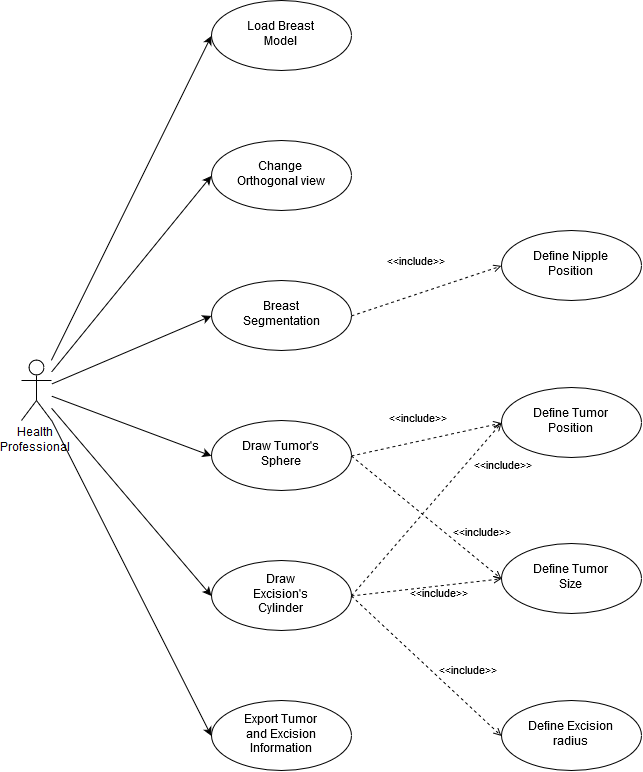
\includegraphics[width=0.7\textwidth]{Use_Cases}
    \caption[BCS planning tool Use Cases]{Use cases for the BCS planning tool}
    \label{fig:use_cases}
  \end{center}
\end{figure}

\subsection{Functional Constraints}

The developed tool have some constraints, due to the representation of the breast model as a point cloud. Those constraints are presented below:
\begin{itemize}
\item When selecting both the nipple and tumor position, must be a point from the model's point cloud;
\item The calculation of the breast, tumor and excision volumes are calculated through approximations;
\item When defining the tumor's sphere and the excision's cylinder, the breast boundaries are not taken into account. This way, the defined polygon will be drawn disregarding the point clouds' limits.
\end{itemize}

\section{Non Functional Requirements}

These are the requirements that are not crucial for the normal function of the application but enhance the user's experience. 

\begin{itemize}
\item \textbf{Interface:} The user interface must be intuitive allowing the user to access all the functionalities with the minimal interaction with the tool in a logical way. To enhance this process many of the functionalities despite of being always visible are only enable when the system has enough information to perform it. In some cases the system warns the user to add necessary information before performing the task;
\item \textbf{Maintenance:} The tool was developed in a way to easily modify the implemented functionalities of the system;
\item \textbf{Expandability:} The tool was developed in a way to easily extend or add additional functionalities to the system;
\item \textbf{Efficiency:} The tool performs all the system's function on a short time.
\end{itemize}


\section{Application Flow}

The flow presented in Figure \ref{fig:tool_flow} shows the required steps to perform the BCS planning. All the tasks not presented on the flow are done at any moment after loading the breast's model.

\begin{figure}[!h]
\begin{center}
    \leavevmode
    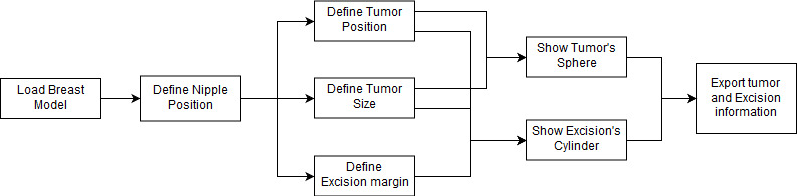
\includegraphics[width=1.0\textwidth]{tool_flow_2}
    \caption[BCS planning tool flow]{Tool flow with the required steps to perform the BCS planning}
    \label{fig:tool_flow}
  \end{center}
\end{figure}

\section{Development}

The frameworks used for the development of the described application are explained below and were implemented using C++. A few frameworks such as Qt and VTK were also used in order to simplify the tool's interface development.

\subsection{System Documentation}
All the developed codes were written clearly and in a straightforward way in order to allow a intuitive and fast reading of each function and described object.

\subsection{C++}
All the required functions where declared on the header files and respectively implemented on the correspondent \textit{cpp} file. Besides the utilization of this types of file, there is a main file responsable for the execution of the interface and all the functions associated with it, and a \textit{ui} (user interface) file where the interface was designed.

\subsubsection{Code comments}
The code comments, as a way of code documentation, are only used when necessary decreasing the amount of visual barriers, often associated with mathematical formulas or required calculations on the 3D space.

\subsection{Used Frameworks}

\subsubsection{Qt}

Qt allows the development of multi-platform applications and interfaces based on C++ in a simple and fast way \footnote{\url{http://doc.qt.io/}}.

\subsubsection{VTK}
The Visualization Toolkit (VTK) is an open-source software system used for 3D computer graphics, image processing, and visualization that consists of a C++ class library including several interpreted interface layers \footnote{\url{http://www.vtk.org/documentation/}}. VTK integrates other frameworks such as Qt, also used for the development of this application.

\subsubsection{Boost library}
Boost library is a C++ set of libraries that allows an easy utilization of linear algebra, image processing and multithreading. These libraries are required for the utilization of VTK and Qt frameworks.

\section{Interface}

Figure \ref{fig:tool_interface} shows the interface of the main functionalities of the tool. When launching the tool, the initial window will be displayed, where it is only possible to load a breast's point cloud \subref{fig:initial_view}. After loading the breast's model, the nipple's position feature is enabled. The breast's point cloud is also displayed on the visualization area. A selection point view for the nipple position is presented in \subref{fig:point_selection}. For the tumor position a similar view will be displayed with the breast seen from a frontal position. After defining the nipple position, the breast can be divided into quadrants. This can be seen through planes drawn over the breast in \subref{fig:segmentation_view}. In order to do the tumor definition, tumor position is selected as well as a tumor size. If one of the fields is not checked, a warning window will be displayed \subref{fig:warning_alert}. When all the fields are completed, a tumor's sphere can be drawn and displayed over the breast on the visualization area \subref{fig:tumor_view}. Last, but not least, when selecting an excision margin, the excision's cylinder is drawn \subref{fig:excision_view}.

Regarding the interface, this was created considering the target group and adapted according to its propose. One of the aspects that were took into consideration was the used icons. Due to the lack of materials guidelines and icons to represent some of the intended actions, some icons used in the tool were created in order to overcome that lack and the ones that already existed were adjusted to provide an overall consistency among all the tool. Other human-computer iteration principles were considered as the representation of already clicked buttons, and the pop-up of warning and dialog messages to inform the user about any error or task completion. The tool's interface is displayed in Figure \ref{fig:loaded_r}, where the interaction panels are delimited and coupled with a label.

\begin{figure}[!h]
\centering
\scalebox{1.1}{%
\begin{tabular}{ll}
\subfloat[Initial view]{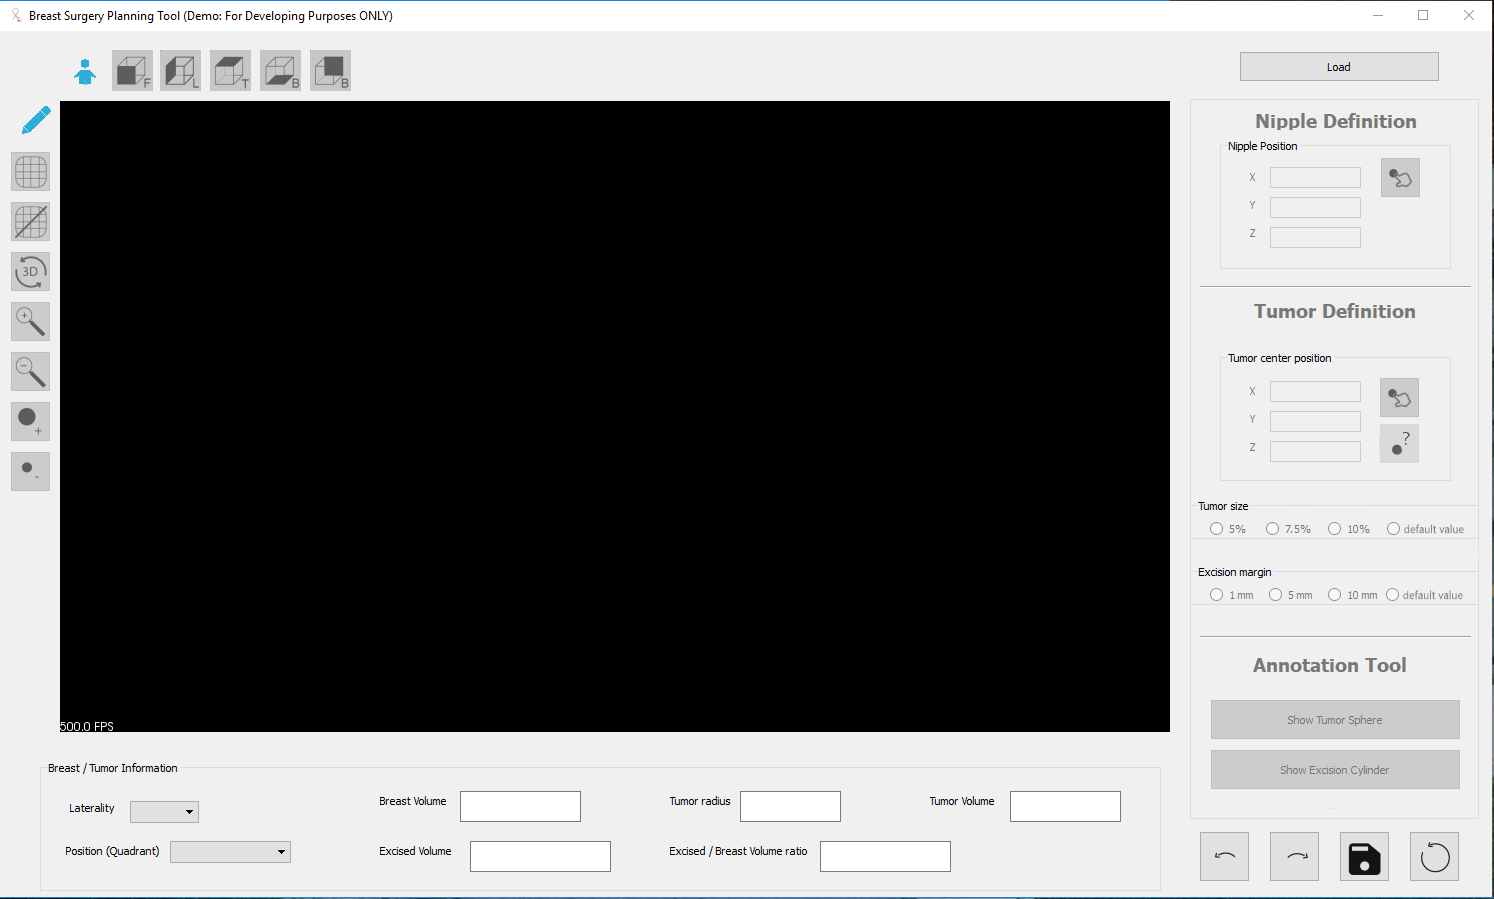
\includegraphics[width = 3in]{initial_r2}\label{fig:initial_view}} &
\subfloat[Point Selection View]{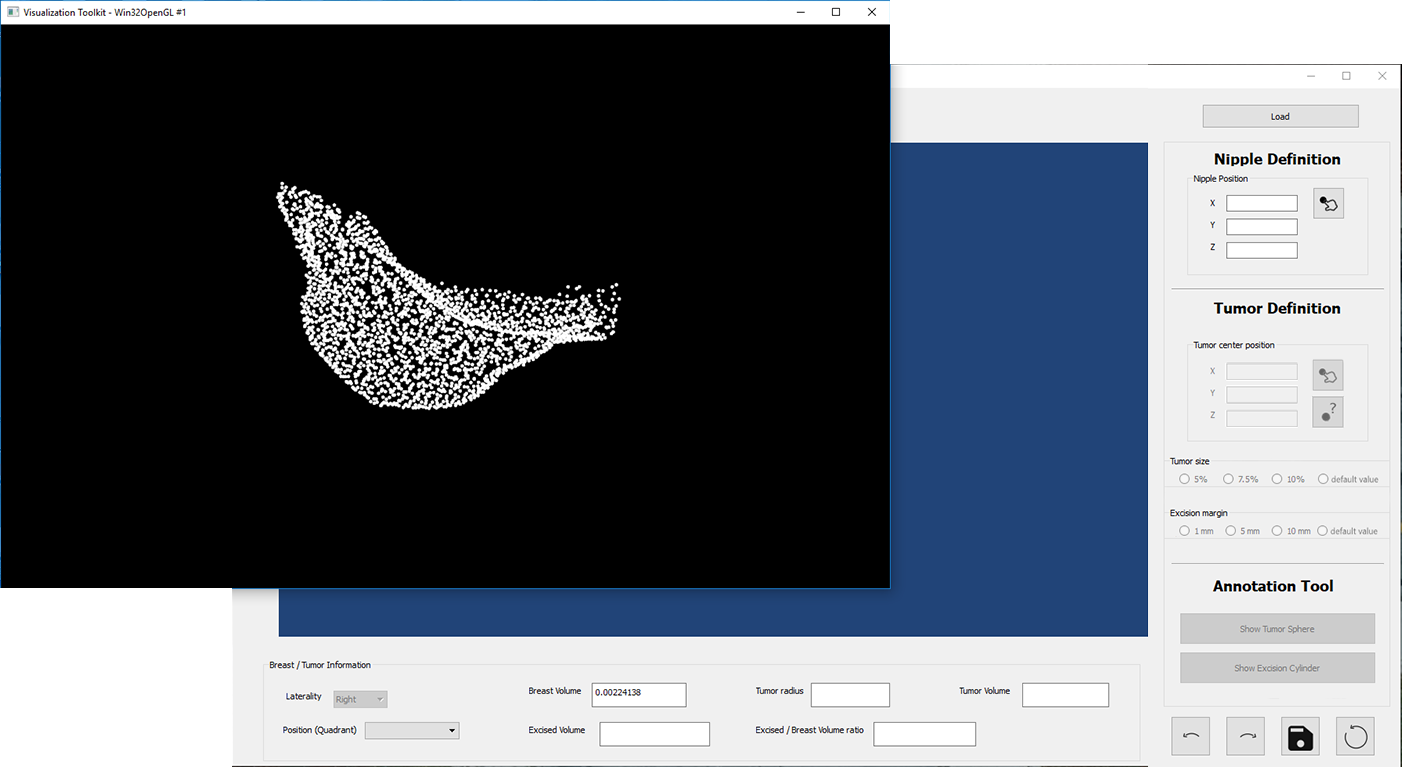
\includegraphics[width = 3in]{point_selection_r2}\label{fig:point_selection}}\\
\subfloat[Breast Segmentation View]{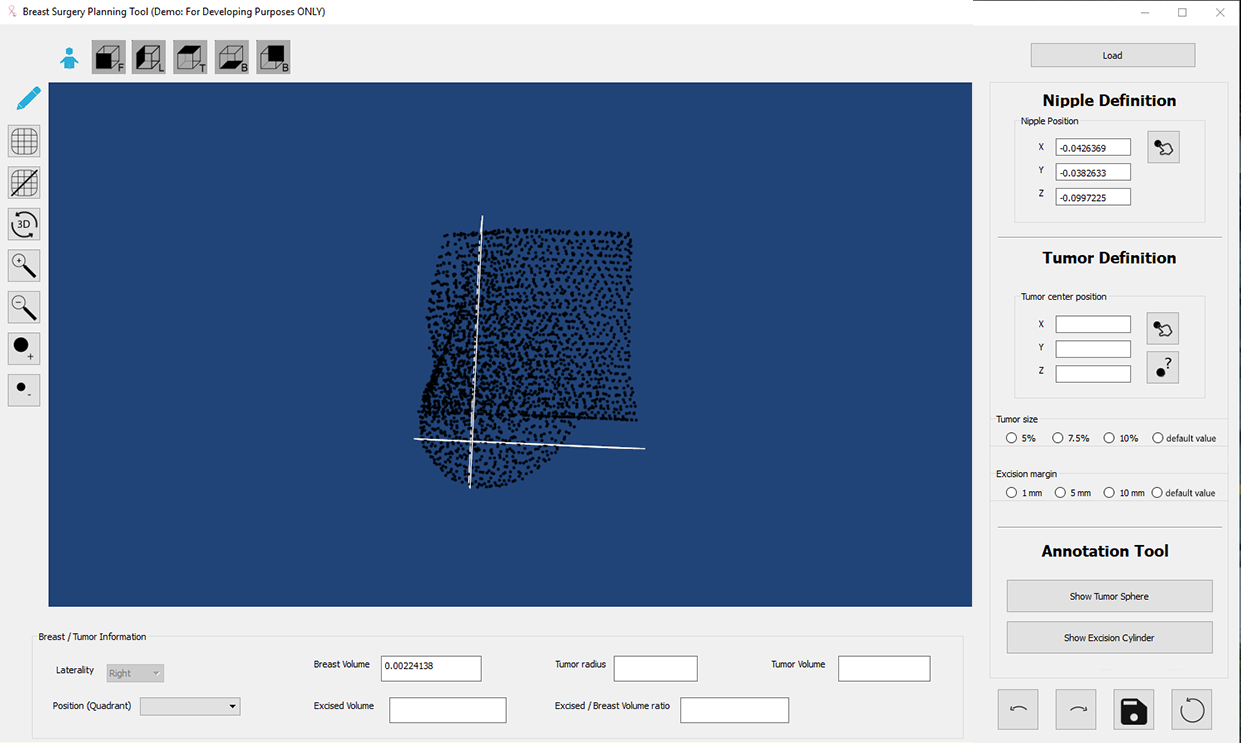
\includegraphics[width = 3in]{segmentation_r2}\label{fig:segmentation_view}} &
\subfloat[Warning Alert]{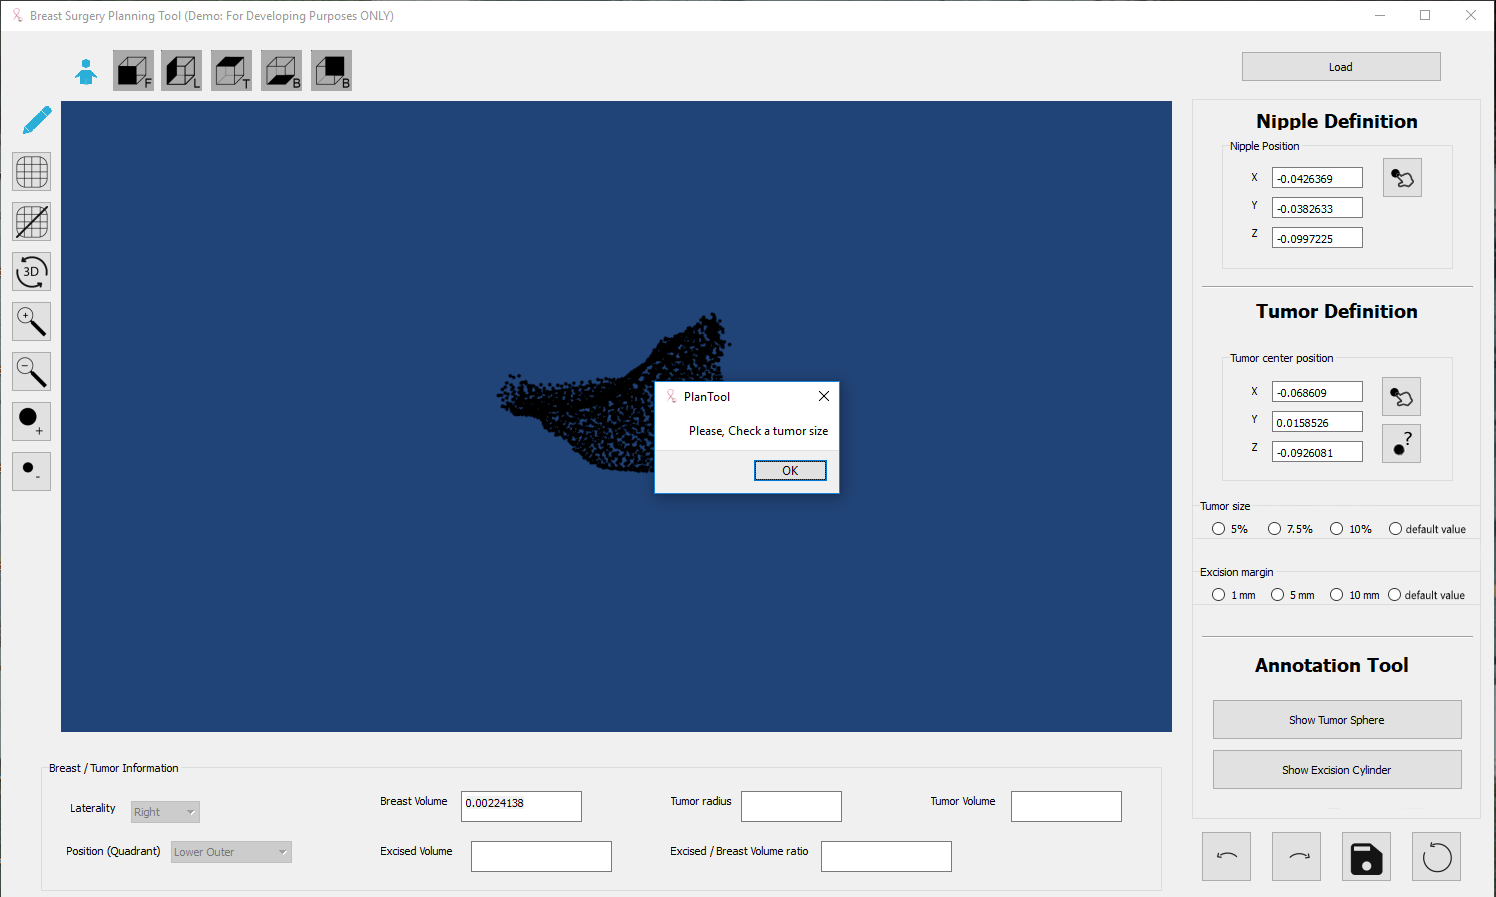
\includegraphics[width = 3in]{warning_r2}\label{fig:warning_alert}}\\
\subfloat[Tumor's view]{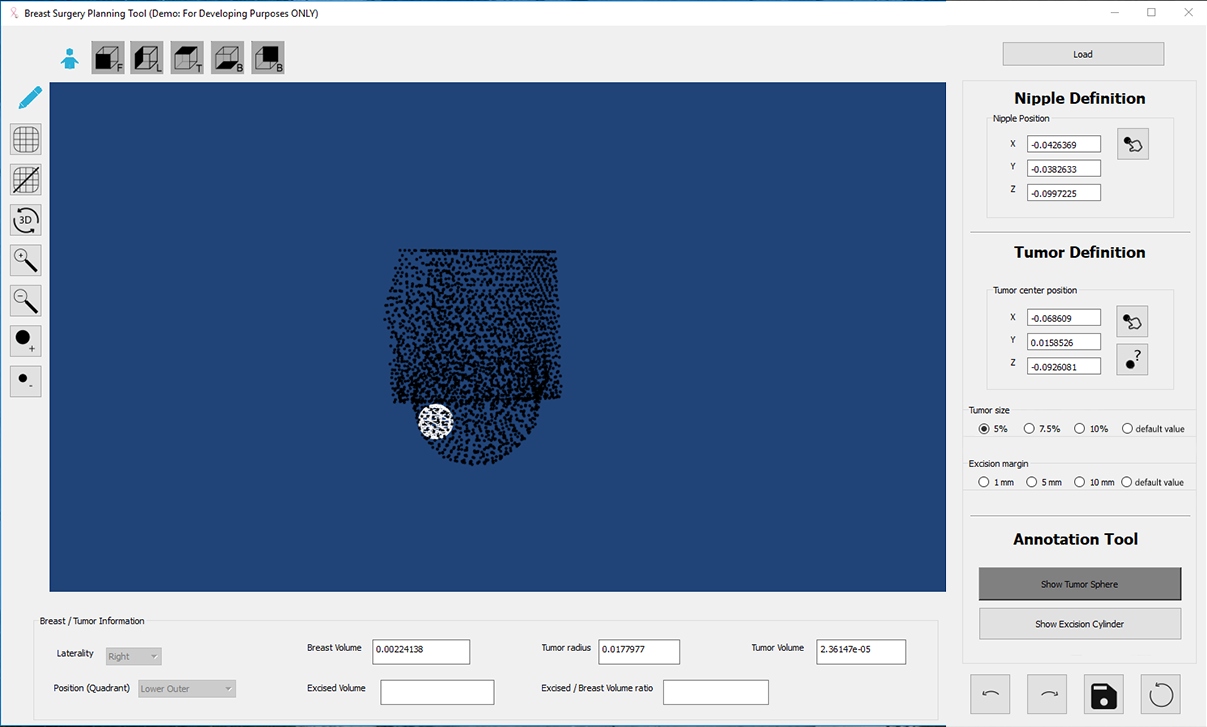
\includegraphics[width= 3in]{tumor_def_r2}\label{fig:tumor_view}} &
\subfloat[Excision's view]{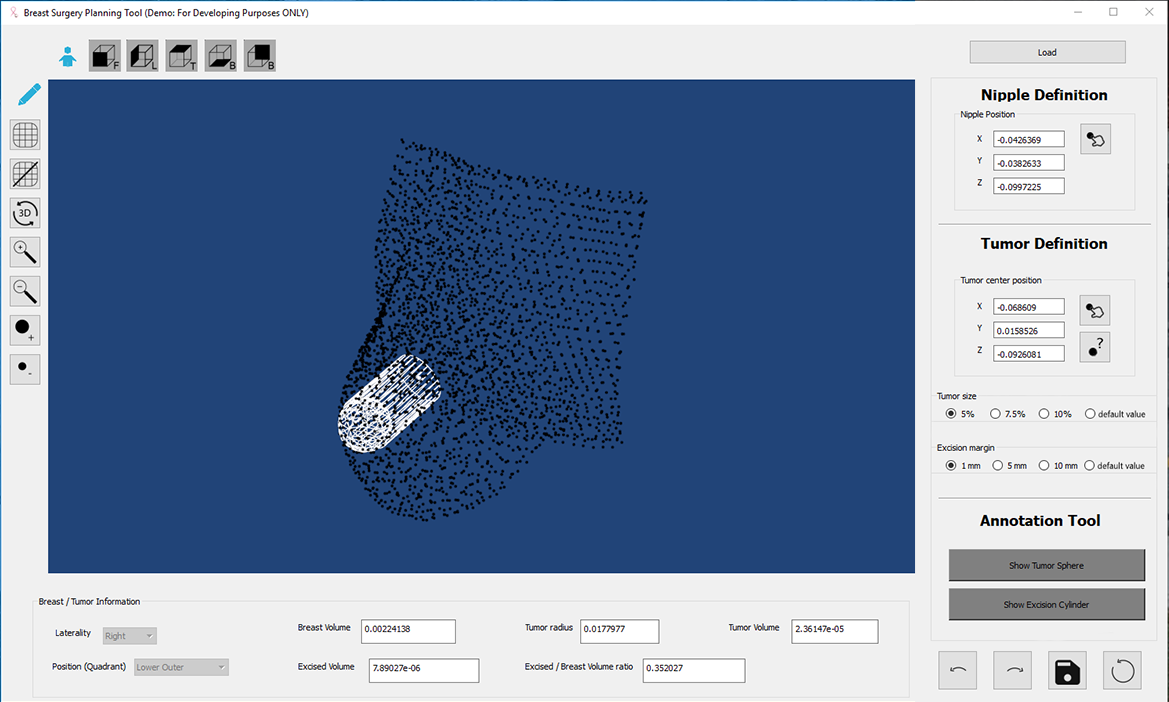
\includegraphics[width = 3in]{cylinder_def_r2}\label{fig:excision_view}} \\
\end{tabular}
}
\caption[BCS planning tool interface]{Interface of several views of the BCS planning tool}
\label{fig:tool_interface}
\end{figure}

\begin{figure}[!h]
\centering
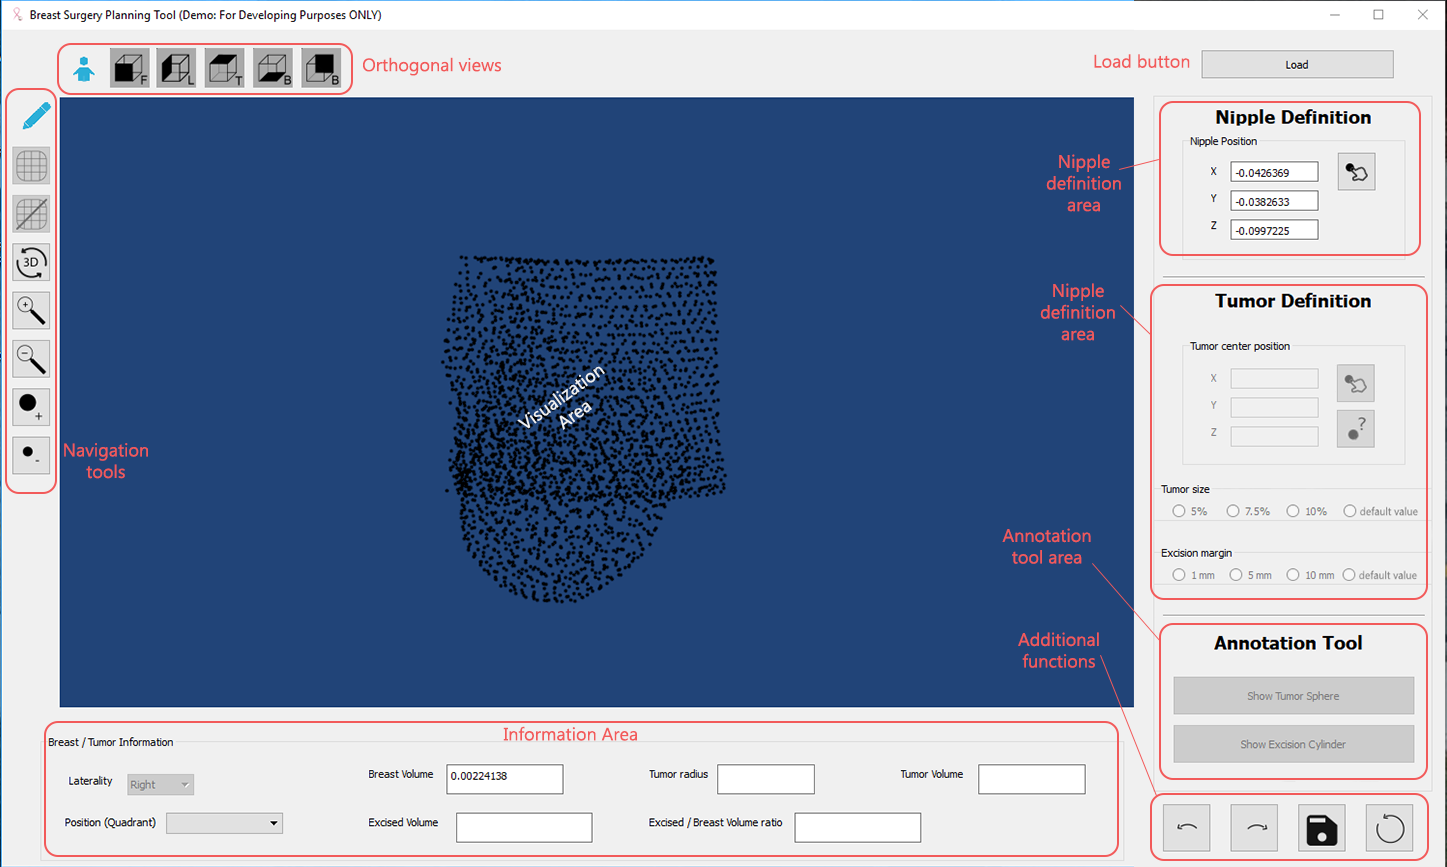
\includegraphics[width=1.0\textwidth]{loaded_r2}
    \caption[BCS planning Tool Interface]{BCS Tool Interface}
    \label{fig:loaded_r}
\end{figure}


\section{Summary}
In this chapter the developed BCS planing tool was presented as well as both functional and non functional requirements, application flow, the frameworks that were used. Also some considerations regarding its development and implementation are described as well as some interfaces of the application.

One of the most valuable functionalities that the tool can be equipped with is to allow the simulation and further visualization of the breast's deformations predicted by the models described in chapter \ref{chap:method}.
\chapter{Methodology}\label{chap:method}

\section*{}
In this chapter all the process that led to achieving the main goal of the thesis, predict the deformations caused by BCS is described in detail.
In order to plan such process, the study on breast cancer and how to represent the Breast as a 3D model will be used, as well as the developed tool described in chapter \ref{chap:tool}.

The applied methodology is divided in 3 fundamental parts: a dataset preparation to feed the following steps, the application of Machine Learning in order to predict the deformations on the patient's breasts caused by the BCCT, and the validation of the obtained results through several metrics. Those three steps are represented on Figure \ref{fig:method_FC} and are detail through the several sections on this chapter.

\begin{figure}[!h]
\begin{center}
    \leavevmode
    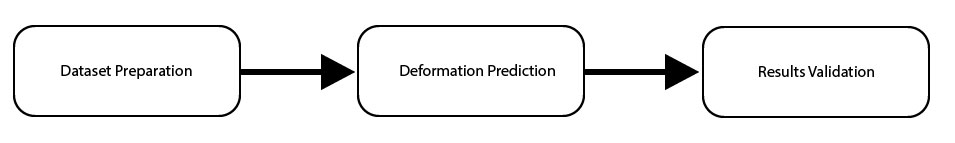
\includegraphics[width=0.85\textwidth]{method_FC}
    \caption[Flowchart of the applied methodology]{Flowchart of the applied methodology}
    \label{fig:method_FC}
  \end{center}
\end{figure}

\section{Dataset Preparation}\label{sec:dataset_prep}

In order to further apply machine learning techniques to predict the deformations on the patient's breast, a semi-synthetic dataset was prepared. Despite of existing a few datasets with 3D models of the breast, they are constructed based on a generic shape of the breast with some deformations applied to it. Although the great amount of studied deformations, they are still unable to represent the variability and diversity that may be found in a semi-synthetic dataset. This created semi-synthetic dataset contains 3D breast models representing the patient's breast before and after the surgery. The pre-surgical models in the dataset are based on the real data obtained though MRI data of a few patients. The pos-surgical models are generated by taking as parameters the hypothetical tumor's location and volume and the breast's density. Considering different parametrization, each pre-surgery model of the dataset defer from other regarding the following features:
\begin{itemize}
\item breast's density,
\item breast's volume,
\item breast's laterality,
\item tumor's position
\item tumor's volume.
\end{itemize} 
The pos-surgery 3D models of the breast are obtained though a biomechanical simulation of the wound healing based on the pre-surgical models generated through the patients' MRI data. The BCS planning tool described in chapter \ref{chap:tool} was used to generate the hyphothetical tumor's location and volume. The pre-surgery models will be used to simulate the pos-surgery models alongside with the hyphotetical tumor's location and size through a biomechanical healing simulator described in \cite{Vavourakis2016}. Figure \ref{fig:data_WF} illustrates the workflow of the steps pursued for preparing the dataset.

\begin{figure}[!h]
\begin{center}
    \leavevmode
    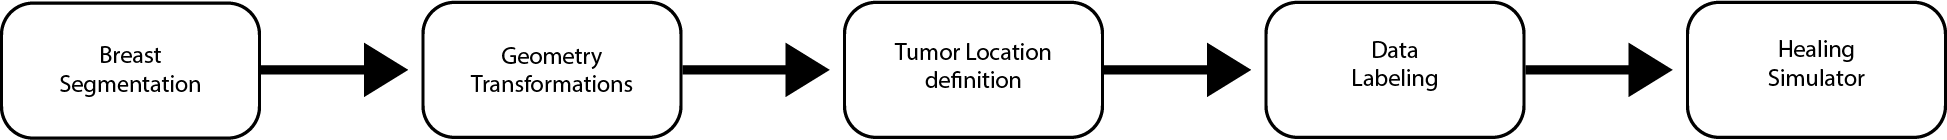
\includegraphics[width=1.0\textwidth]{data_WF}
    \caption[Flowchart for the dataset generation]{Flowchart for the dataset generation}
    \label{fig:data_WF}
  \end{center}
\end{figure}

Initially, it is necessary to segment the breast outline from background of the MRI data for each initial real patient. Further, a 3D model is reconstructed from the segmented data. However, since the MRI is taken as the patient is lied in prone position, it is necessary to apply a geometry deformation to represent the breast in a supine configuration. With the proper geometry, the tumor must be defined in the specific breast, that therefore will be labelled according with the healthy and damaged portions of the breast. At last, the wound healing simulation will be performed in order to generate the pos-surgical model of the breast.


\subsection{Breast segmentation}

As described before, the pre-surgical 3D models of the patients' breast were constructed based on MRI data segmentation. The breast segmentation is performed by annotating both the breast and the pectoral muscle. The annotation included both left and right breast with the respective nipple and had as lateral boundaries the left and right latissimus dorsi. The pectoral muscle included both the right and left major and minor pectoral muscles. Figure \ref{fig:latissimus} depicts the anatomical structure mentioned during segmentation. The result of a patient annotation used to generate the breast's point cloud is shown in Figure \ref{fig:pre_model_annotation}.

\begin{figure}[!htb]
\begin{center}
    \leavevmode
    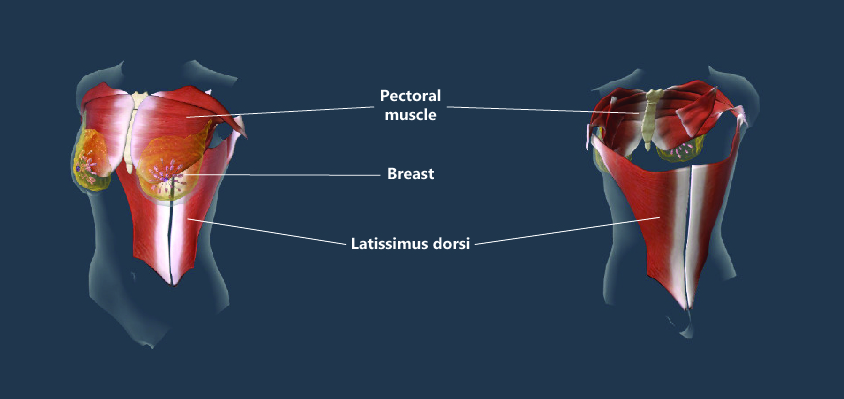
\includegraphics[width=0.85\textwidth]{latissimus}
    \caption[Representation of the Breast, Pectoral muscle and Latissimus Dorsi]{Representation of the Breast, Pectoral muscle and Latissimus Dorsi}
    \label{fig:latissimus}
  \end{center}
\end{figure}

\begin{figure}[!htb]
\begin{center}
    \leavevmode
    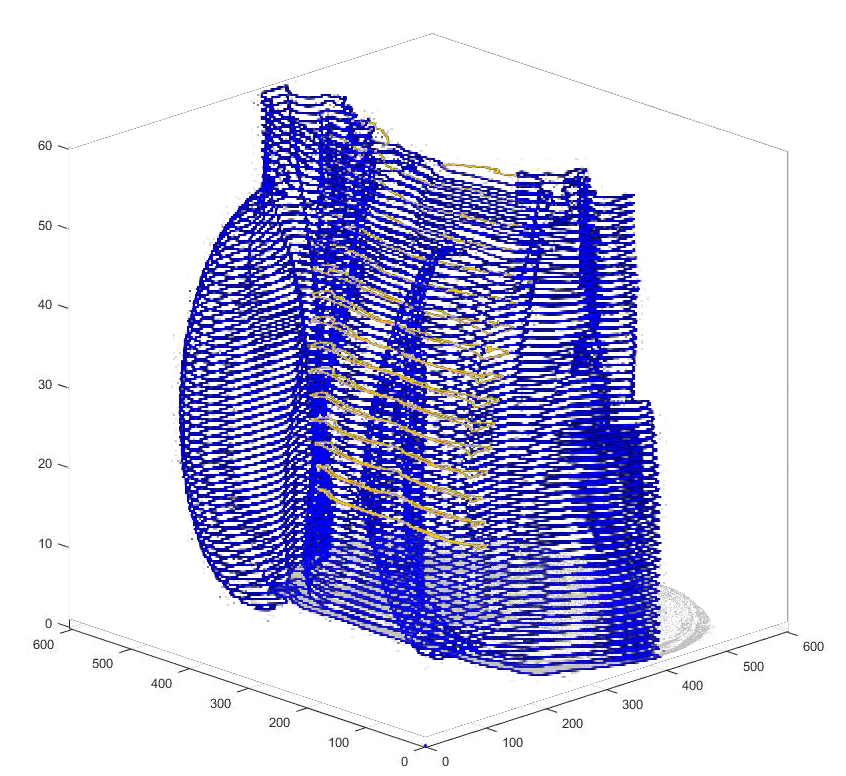
\includegraphics[width=0.45\textwidth]{pre-model}
    \caption[Breast Segmentation result]{Breast Segmentation result for one of the patients}
    \label{fig:pre_model_annotation}
  \end{center}
\end{figure}

All the annotations were made using MARge Tool to appear in \cite{marge}, whose interface is displayed in Figure \ref{fig:marge}.

\begin{figure}[!h]
\begin{center}
    \leavevmode
    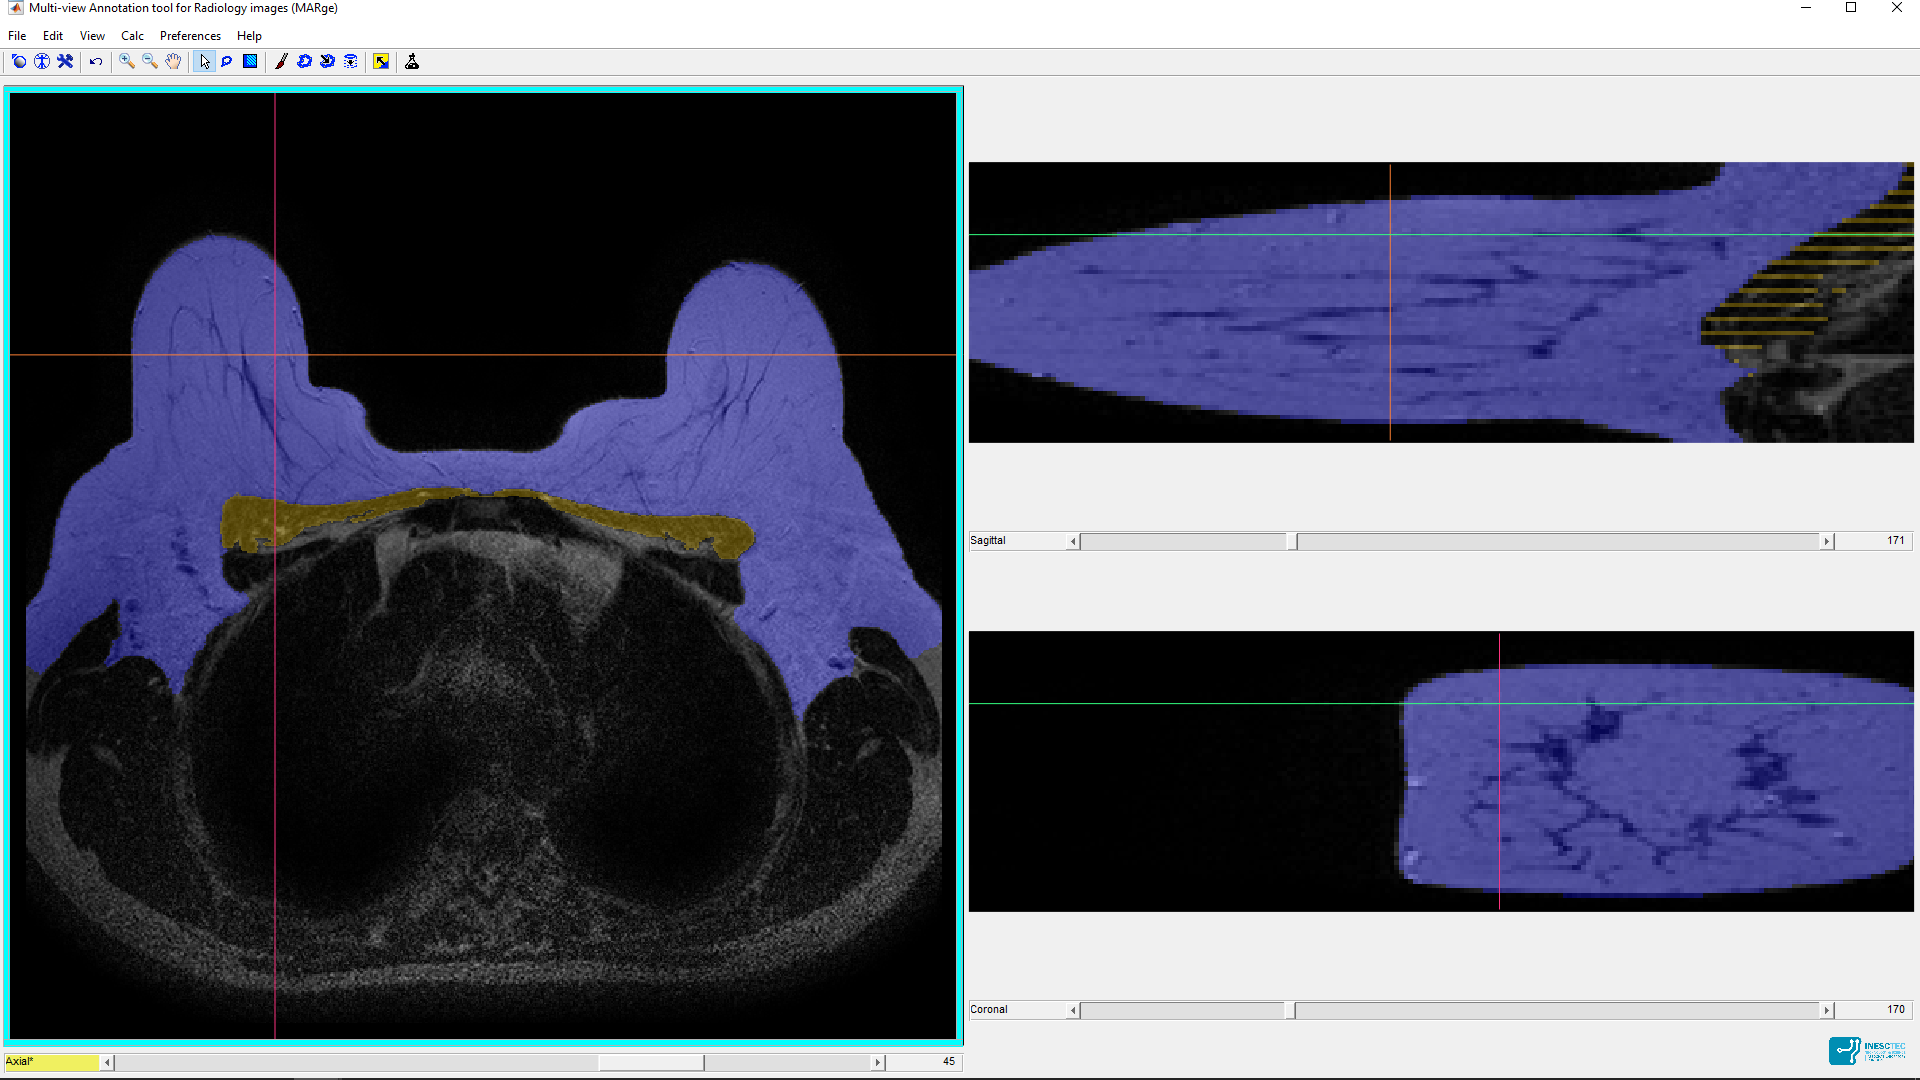
\includegraphics[width=0.70\textwidth]{marge}
    \caption[Interface of MARge tool used for the breast segmentation]{Interface of MARge tool used for the breast segmentation}
    \label{fig:marge}
  \end{center}
\end{figure}

\subsection{Geometry Transformations}\label{subsec:geometry_transf}

After the segmentation of the patient's MRI data, the meshes regarding the pre-surgery models were generated. While the MRI acquisition is done in prone, the tumor definition and posteriorly the surgical simulation need the model in a supine geometry. The transformation between the prone and the supine geometries were performed recurring to a Bio-mechanical simulator described in \cite{Vavourakis2016}. In order to perform these transformation a virtually state known as unloaded geometry was required. In the unloaded geometry, the force of gravity and other tension or stress forces are ignored \cite{Iben2016}. The same biomechanical simulator is used to generate the pre-surgical model in a upright geometry (from the unloaded model) that will be further used. The aesthetic evaluation of the breast is performed in a upright position. The impact of changing the direction of gravity vector to a breast model is depicted in Figure \ref{fig:breast_geometry}.

\begin{figure}[!htb]
\centering
\scalebox{0.73}{%
\begin{tabular}{cc}
\subfloat[3D view of Prone geometry]{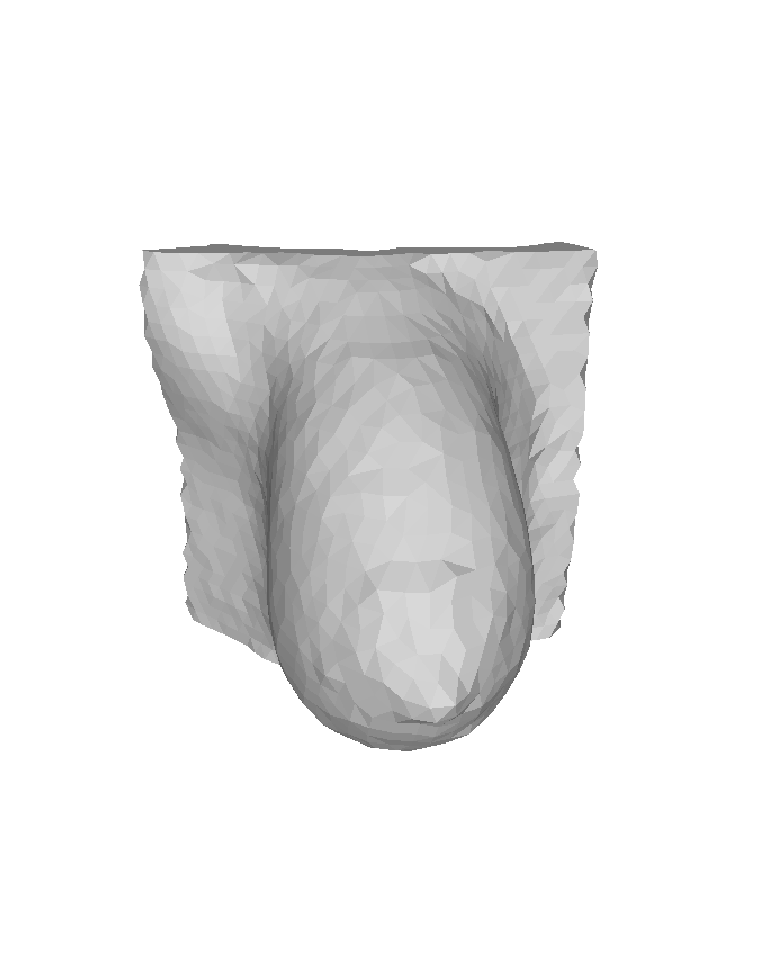
\includegraphics[width = 2in]{prone}\label{fig:prone}} &
\subfloat[Lateral view of Prone geometry]{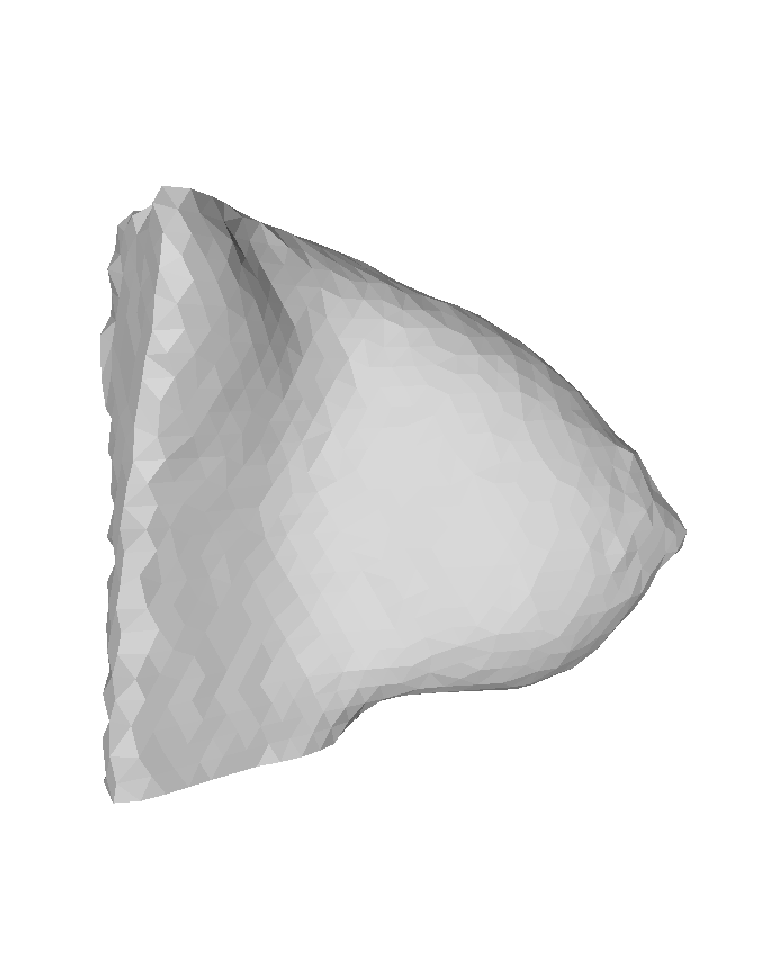
\includegraphics[width = 2in]{prone_l}\label{fig:prone_l}}\\
\subfloat[3D view of Unloaded geometry]{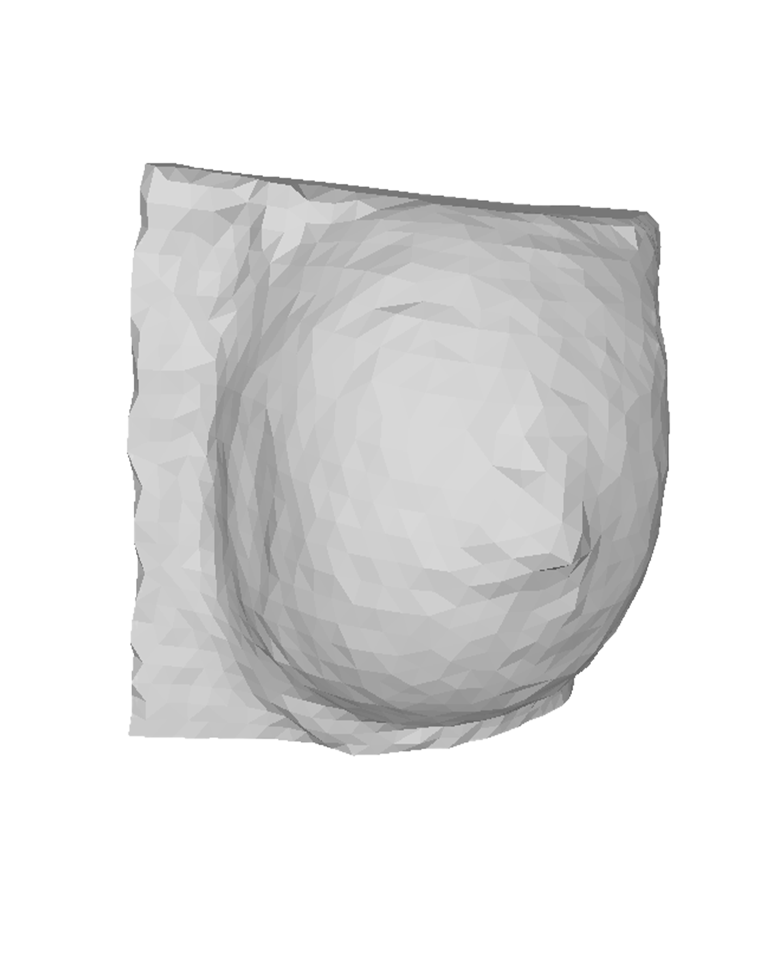
\includegraphics[width = 2in]{unloaded}\label{fig:unloaded}} &
\subfloat[Lateral view of Unloaded geometry]{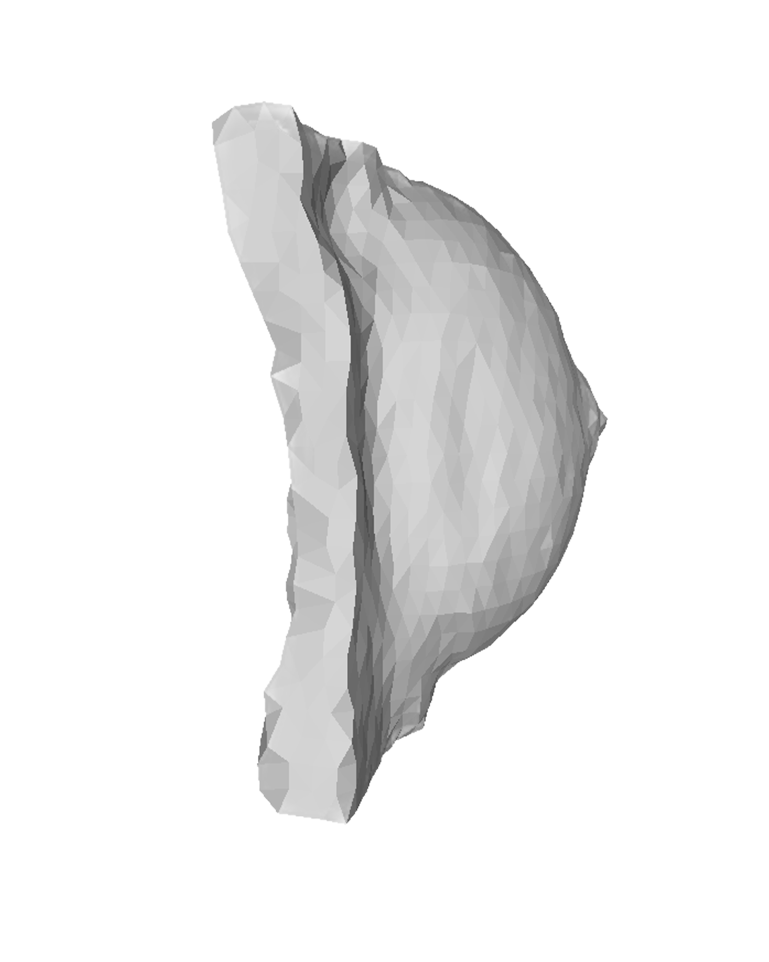
\includegraphics[width = 2in]{unloaded_l}\label{fig:unloaded_l}}\\
\subfloat[3D view of Supine geometry]{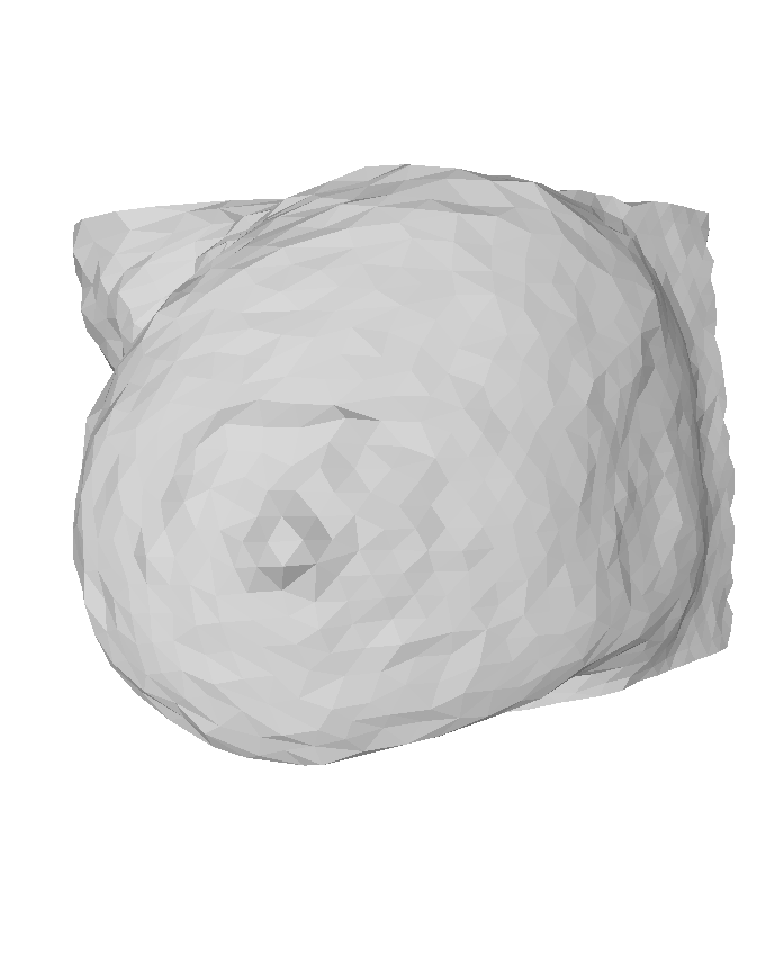
\includegraphics[width = 2in]{supine}\label{fig:supine}} &
\subfloat[Lateral view of Supine geometry]{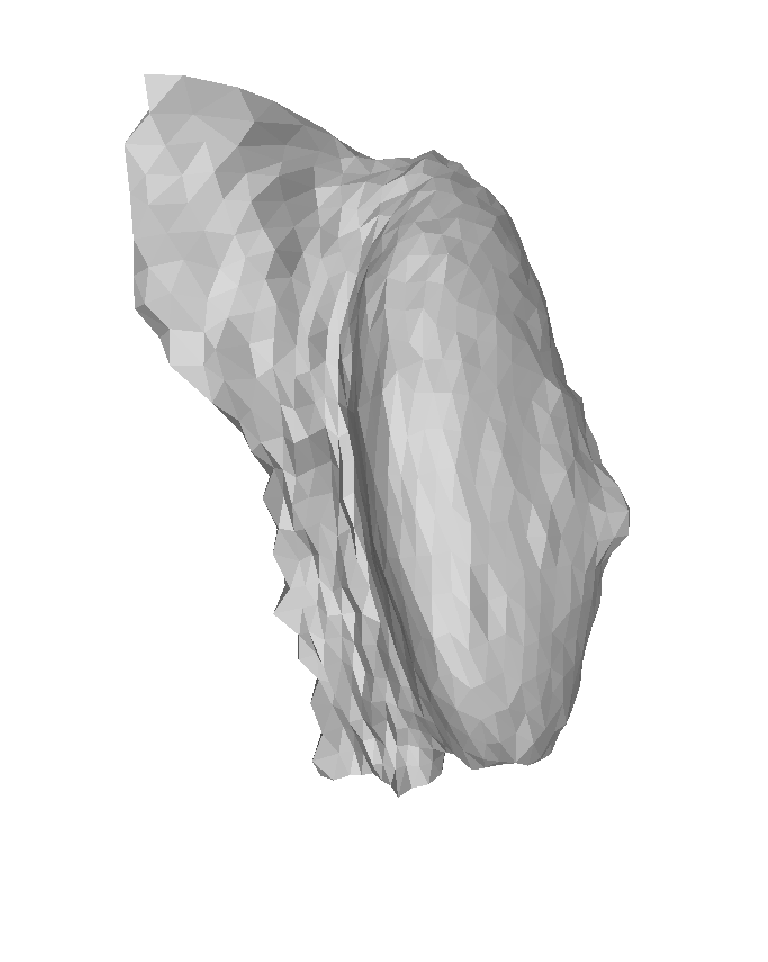
\includegraphics[width = 2in]{supine_l}\label{fig:supine_l}}\\
\subfloat[3D view of Upright geometry]{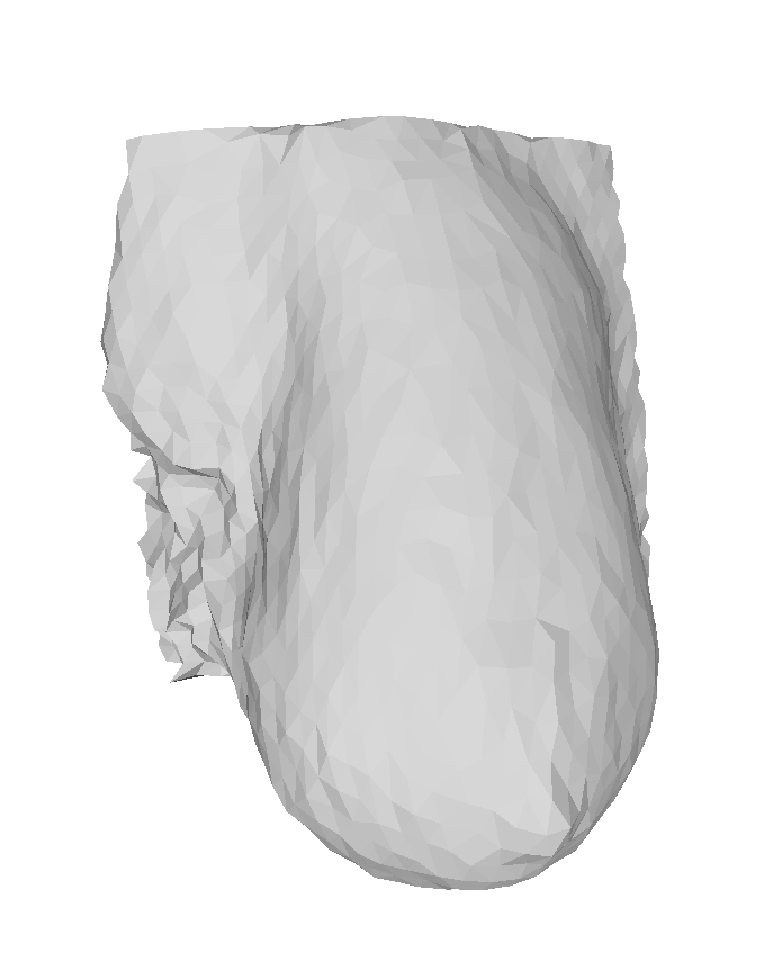
\includegraphics[width = 2in]{upright}\label{fig:upright}} &
\subfloat[Lateral view of Upright geometry]{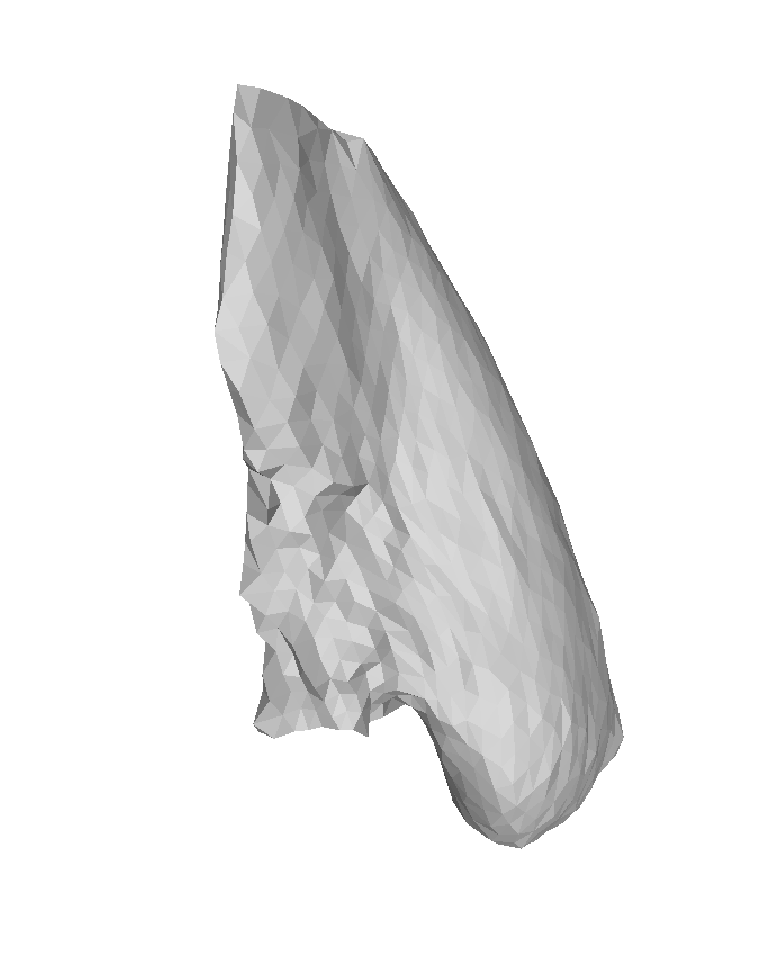
\includegraphics[width= 2in]{upright_l}\label{fig:upright_l}}
\end{tabular}
}
\caption[3D breast geometry transformations]{3D breast geometry transformations}
\label{fig:breast_geometry}
\end{figure}


\subsection{Tumor's location definition}\label{subsection:tumor_location}

The tumor definition is done recurring to the tool described in chapter \ref{chap:tool}. The tool will take as input the pre-surgery model in a supine geometry and query the user for a tumor position. By selecting the tumor's position, it will be categorized according to one of the four quadrants of the breast also defined as regions, as shown in Figure \ref{fig:regions}:
\begin{itemize}
\item R1 - Upper-Outer quadrant of the breast;
\item R2 - Upper-Inner quadrant of the breast;
\item R3 - Lower-Outer quadrant of the breast;
\item R4 - Lower-Inner quadrant of the breast.
\end{itemize}

\begin{figure}[!htb]
\begin{center}
    \leavevmode
    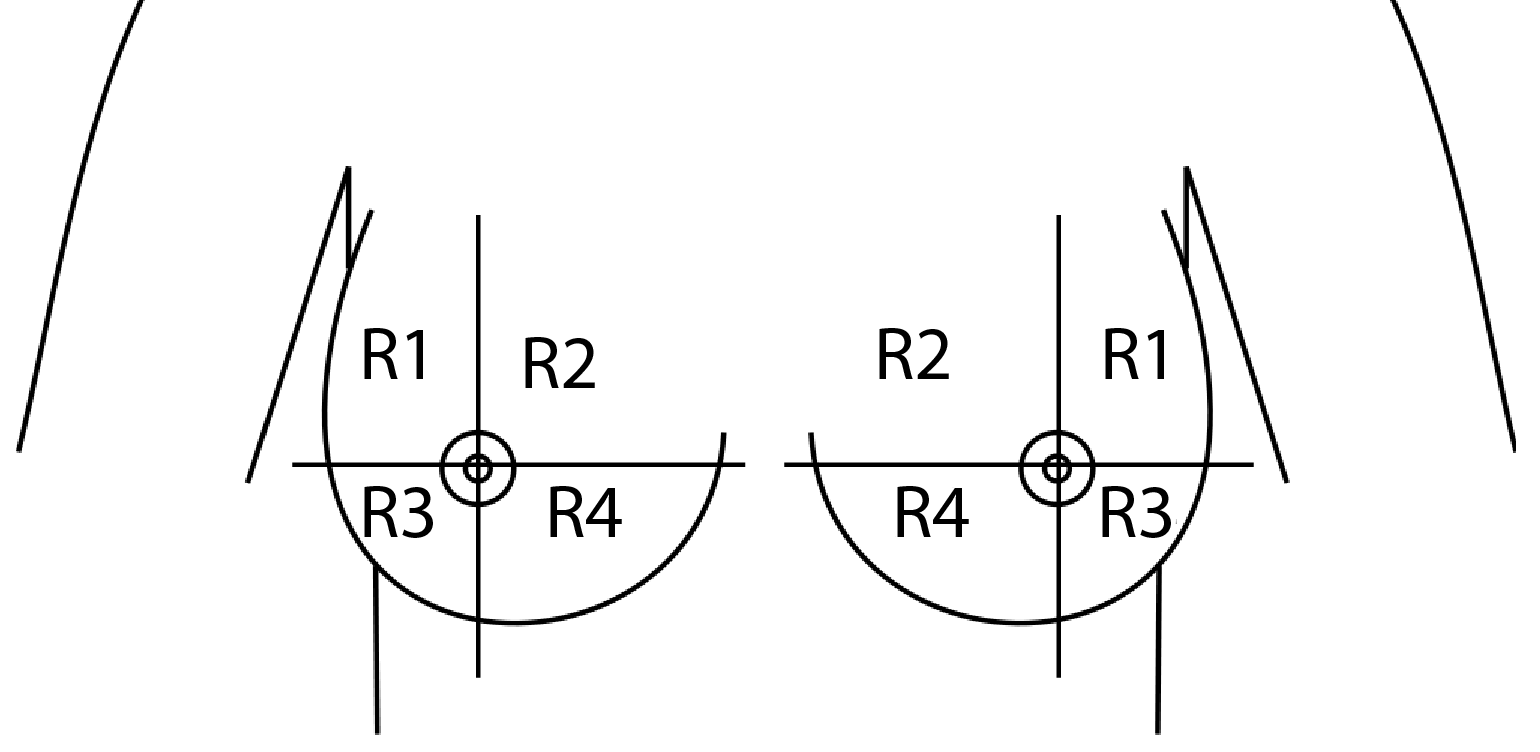
\includegraphics[width=0.55\textwidth]{quadrants}
    \caption[Breast quadrants used for tumor location]{Breast quadrants used for tumor location}
    \label{fig:regions}
  \end{center}
\end{figure}


Thereafter a mesh containing the tumor in the defined region with one of the predefined sizes as follows will be generated:

\begin{itemize}
\item A small size - corresponding to 5\% of the total breast's volume;
\item A medium size - corresponding to 7.5\% of the total breast's volume;
\item And a large size - corresponding to 10\% of the total breast's volume.
\end{itemize}


The percentages used as default for the tumor's size were obtained through discussion with physicians to understand the approximate size of the tumor in different stages of cancer detection.

The produced tumor will be represented by a cylinder centred on the chosen position for the tumor and perpendicular to the chest wall going from the pectoral muscle to the skin contour of the breast. The cylinder's radius is calculated based on the tumor size. All the process is visually supervisioned and the results for the tumor need to be accepted by the user. As result a mesh with exact shape of the one used as input will be generated and posteriorly labelled to be used on the surgical simulation. The labelling process is explained in section \ref{subsection:labelling}.


\subsection{Data Labelling}\label{subsection:labelling}

The labeling is done based on the mesh and what each point and element represents. There will be different labels for surface and volumetric information. The assigned labels indicate the following boundaries of the mesh: front, pectoral muscle or back, left and right or top and bottom. However, the lateral and top and bottom sides of the model are not deformed by the biomechanical neither the wound healing models. The volumetric information is labeled according with the material that it is represented and if it is considered healthy on the case of the breast or damaged on the case of the tumor. While the approach of \cite{Vavourakis2016} divides the volumetric elements in fat and glandular tissue, we assume the same type of material for the all breast. This material's properties are set in order to represent the breast's density according with its ACR (from I to IV). According to \cite{Engineering2008}, using two different material to represent both the fat and glandular tissues, instead of using only one material to represent the whole breast do not significantly affect the results.

In order to visualize the models, a format file exchange is required. While this tool and the one presented on the next subsection require files in a \textit{msh} format, to visualize the models the files must be parsed to a \textit{ply} format. This is done through a parser developed in c++.

After defining damaged or healthy labels, the model will be transformed from supine into the unloaded geometry in order to serve as input on the next step, the surgical simulator, as described in subsection \ref{subsec:geometry_transf}. All the information that is required on this transformations and for the wound healing application (including tumor location and volume and breast's density) is automatically generated by the tool presented in chapter \ref{chap:tool}.


\subsection{Wound healing simulation}\label{subsection:wound_healing_simulation}

The wound healing simulation, where the pos-surgical models are generated, is performed through the application of FEM and Multiscale Mechano-Biological expressions \cite{Vavourakis2016}. 
This will provide what would be the pos-surgical model of the patient's breast roughly 6 months (180 days) after the surgery, taking into consideration the patients breast density, the tumor's location and size that were artificially introduced before. Figure \ref{fig:WHS} demonstrates the breast generated by the wound healing simulation in an upright geometry.

\begin{figure}[H]
    \centering
    \subfloat[Frontal view]{{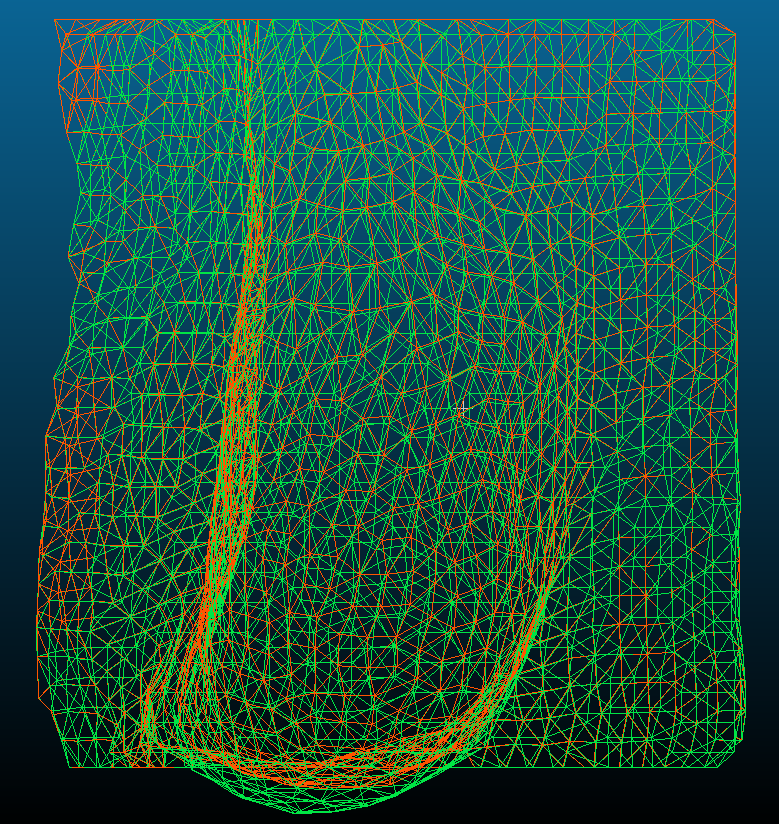
\includegraphics[width=4.5cm, height=4.5cm]{WH_example_frt} }}
    \qquad
    \subfloat[Lateral view]{{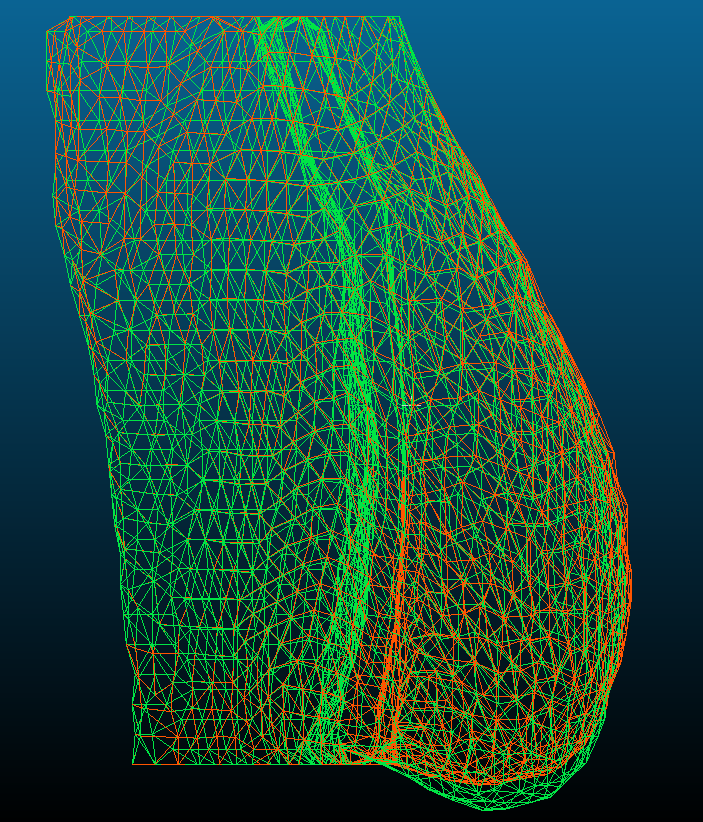
\includegraphics[width=4.5cm, height=4.5cm]{WH_example_lat} }}
    \qquad
    \subfloat[3D view]{{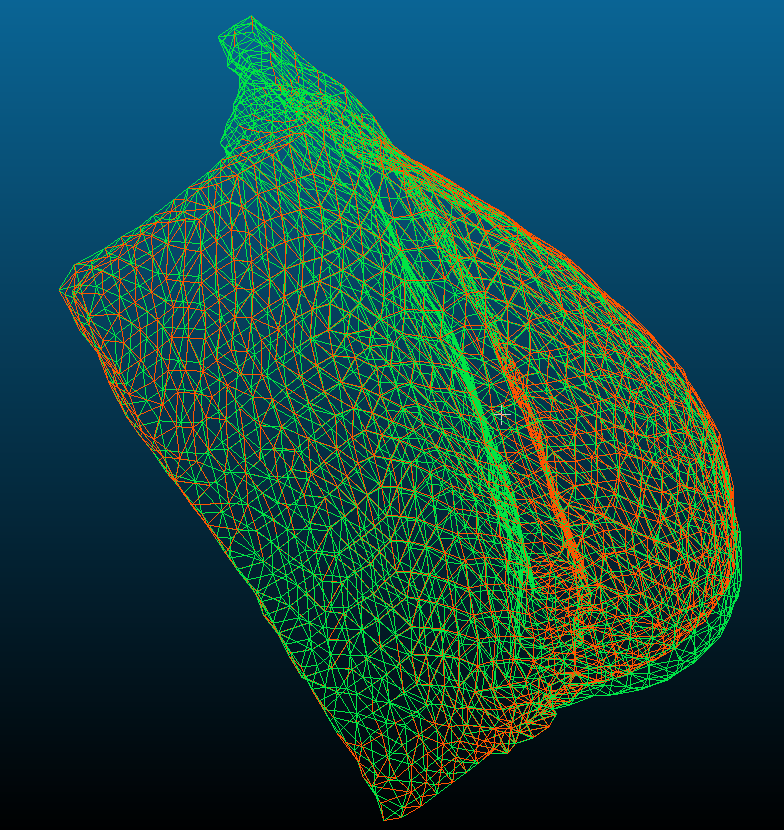
\includegraphics[width=10cm]{WH_example_3d} }}
    \caption[Wound Healing simulation]{Wound Healing simulation - comparison between the pre-surgical mesh (in green) and the pos-surgical mesh (in orange)}
    \label{fig:WHS}
\end{figure}

%\vspace{12mm}


The final dataset currently provides pre and pos-surgical models for a total of 288 possible patients based on 6 initial real patients.

Despite of the annotation for both left and right breasts, using both breasts of the same patient would lead to very similar models to the natural symmetry of the human breasts. The initial real patients used to generate all the scenarios in the semi-synthetic dataset, were choose taking into account their breast volume, being classified as small, medium or large. For each patient regardless the breast size or laterality, models were generated for all the ACR (I to IV), for all the tumor regions (1 to 4) and for all the 3 sizes (1 to 3). These combinations are illustrated in Figure \ref{fig:combinations}.

\begin{figure}[!h]
\begin{center}
    \leavevmode
    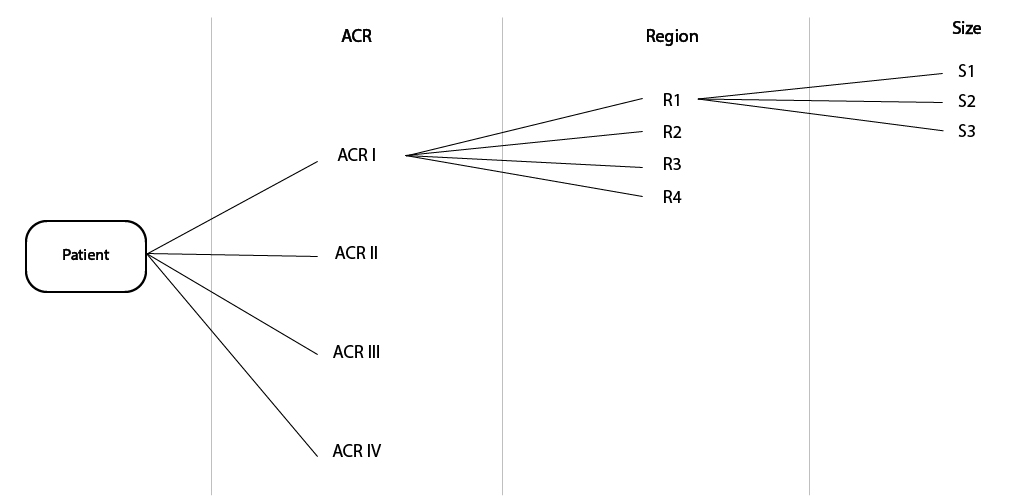
\includegraphics[width=0.8\textwidth]{combinations}
    \caption[Clinical features combinations]{Representation of possible combination of clinical features for the dataset generation}
    \label{fig:combinations}
  \end{center}
\end{figure}

All the dataset preparation steps (described previously in subsections \ref{subsec:geometry_transf}, \ref{subsection:tumor_location}, \ref{subsection:labelling} and \ref{subsection:wound_healing_simulation}) are illustrated in Figure \ref{fig:tld}.

\begin{figure}[!h]
\begin{center}
    \leavevmode
    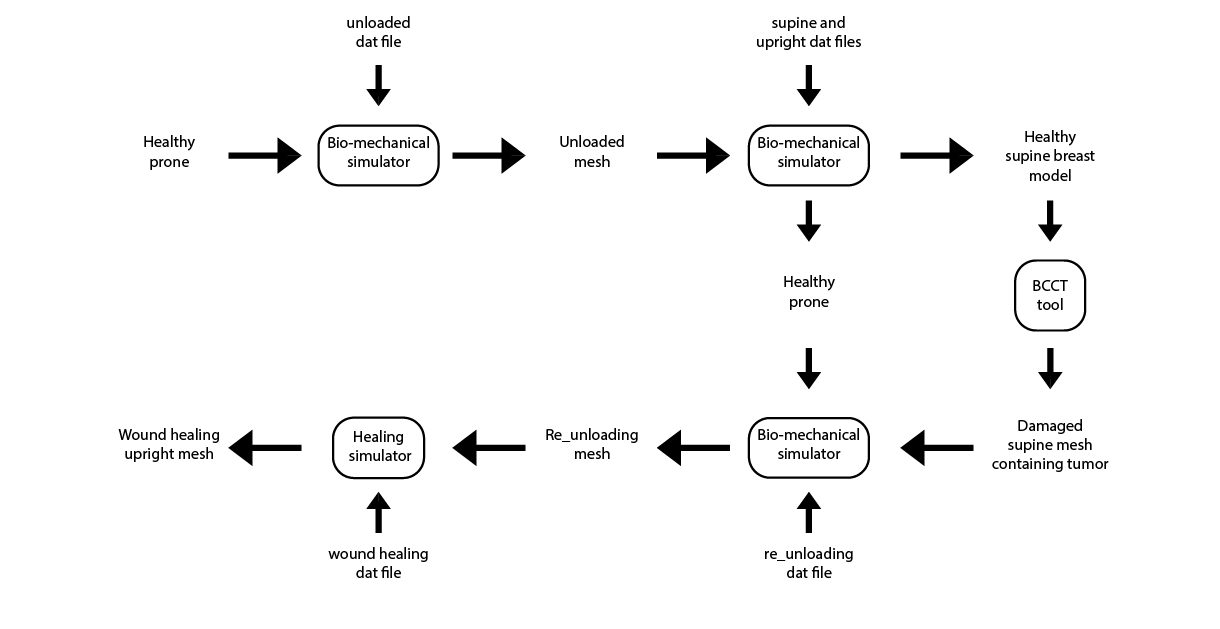
\includegraphics[width=1\textwidth]{TLD_WF-01}
    \caption[Workchart summarizing the breast's geometry transformations and wound healing simulation]{Workchart summarizing the breast's geometry transformations and wound healing simulation. The dat files are used for the Bio-mechanical simulator and the healing simulator containing the bio-mechanical and bio-chemical properties of the model's materials as well as the labelling definition.}
    \label{fig:tld}
  \end{center}
\end{figure}

\vspace{12mm}

\section{Feature Analysis and Feature Construction}

After the construction of the dataset, the data was analysed having into consideration the impact that the clinical features have on the healing simulation. Despite of the already existent and computed features, other features (like the distance between each point and the tumor's position) that were considered promising were computed and used in order to train the machine learning models.

\subsection{Feature Analysis} \label{subsec:feat_analysis}

The analysis of the clinical features was done by comparing the displacement of the corresponding points in the pre and pos-surgical models of the breast between variations of the same patient, where one of the clinical features was changing, and the others were kept the constant. The clinical features that were analysed were the tumor's size, the tumor's region and the ACR of the breast. With this study of the clinical features some conclusions were able to be drawn. The displacement of points resembles a "magnetic field" around the tumor's position and whether the tumor is located on an upper or lower region, the points of the lower region are always moved from their initial position, however, and as expected, when the tumor is located on a lower region, the displacement of the points will be larger and lead to a more profound deformation of the breast, as shown in Figure \ref{fig:region_analysis}. The impact of the tumor size can also be noticed and as expected, a bigger tumor size leads to a greater impact of the breast deformation, represented in Figure \ref{fig:size_analysis}. It is also possible to verify that the breast's density influence the deformations of the breast. A smaller ACR corresponding to a less dense breast will lead to a bigger displacement as represented in Figure \ref{fig:acr_analysis}.

\begin{figure}[!h]
\begin{center}
    \leavevmode
    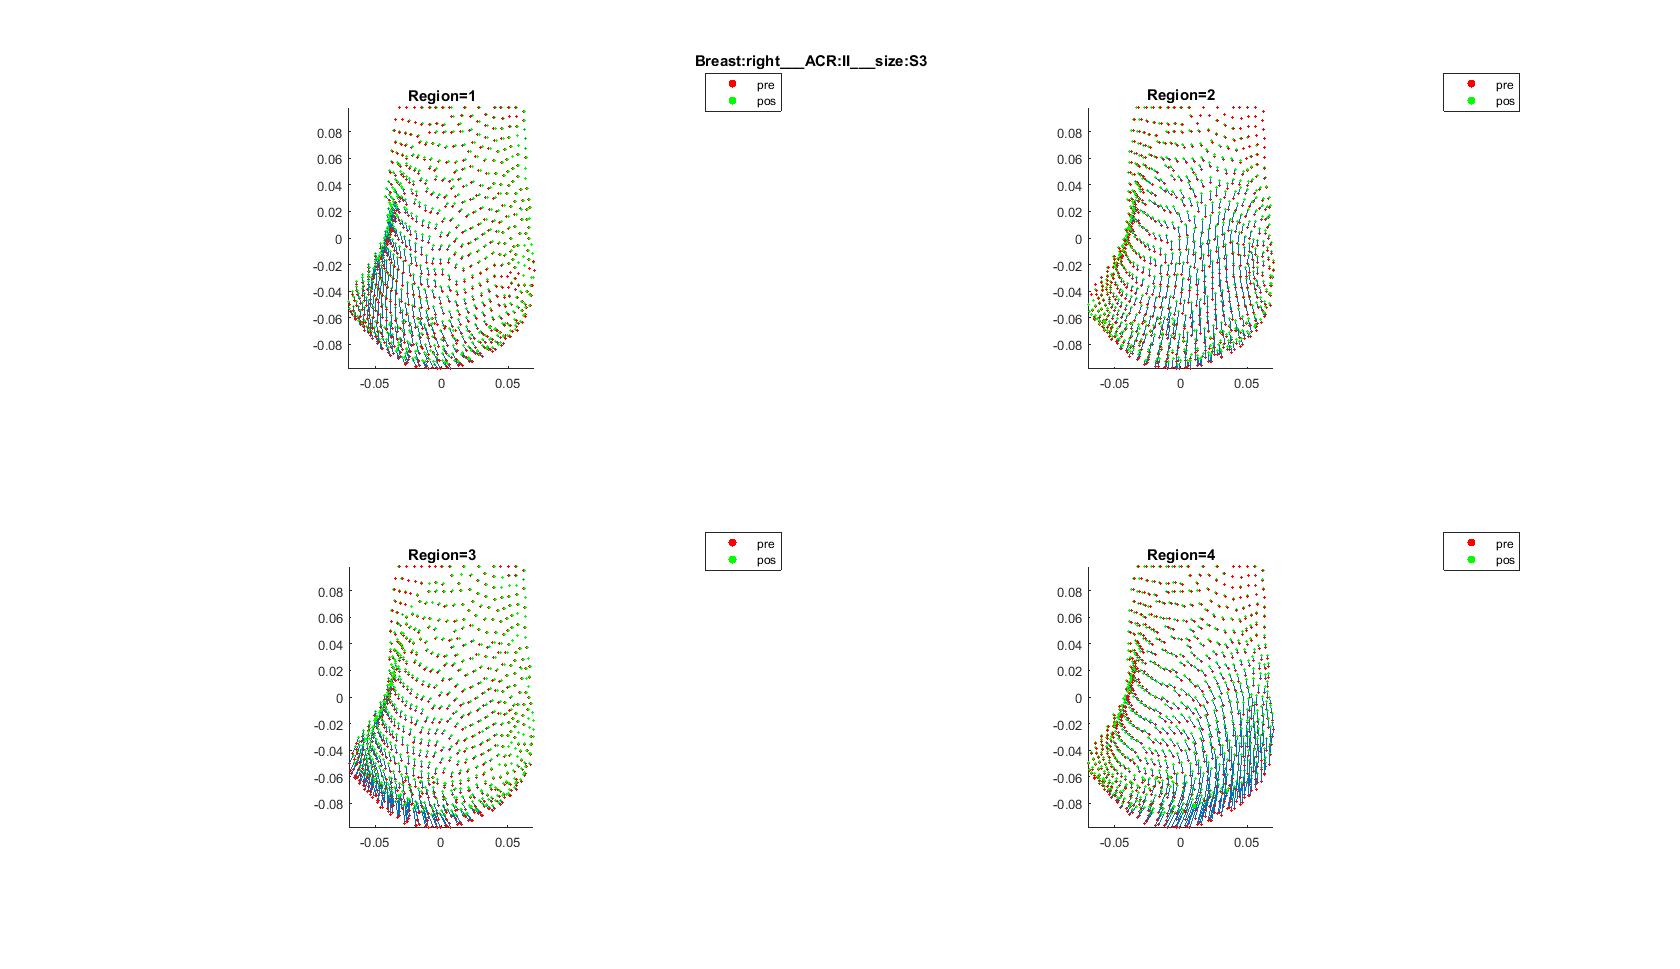
\includegraphics[width=1.2\textwidth]{region_analysis}
    \caption[Example of the impact of tumor's location (region) on the breast's deformation]{Example of the impact of tumor's location (region) on the breast's deformation}
    \label{fig:region_analysis}
  \end{center}
\end{figure}

\begin{figure}[!h]
\begin{center}
    \leavevmode
    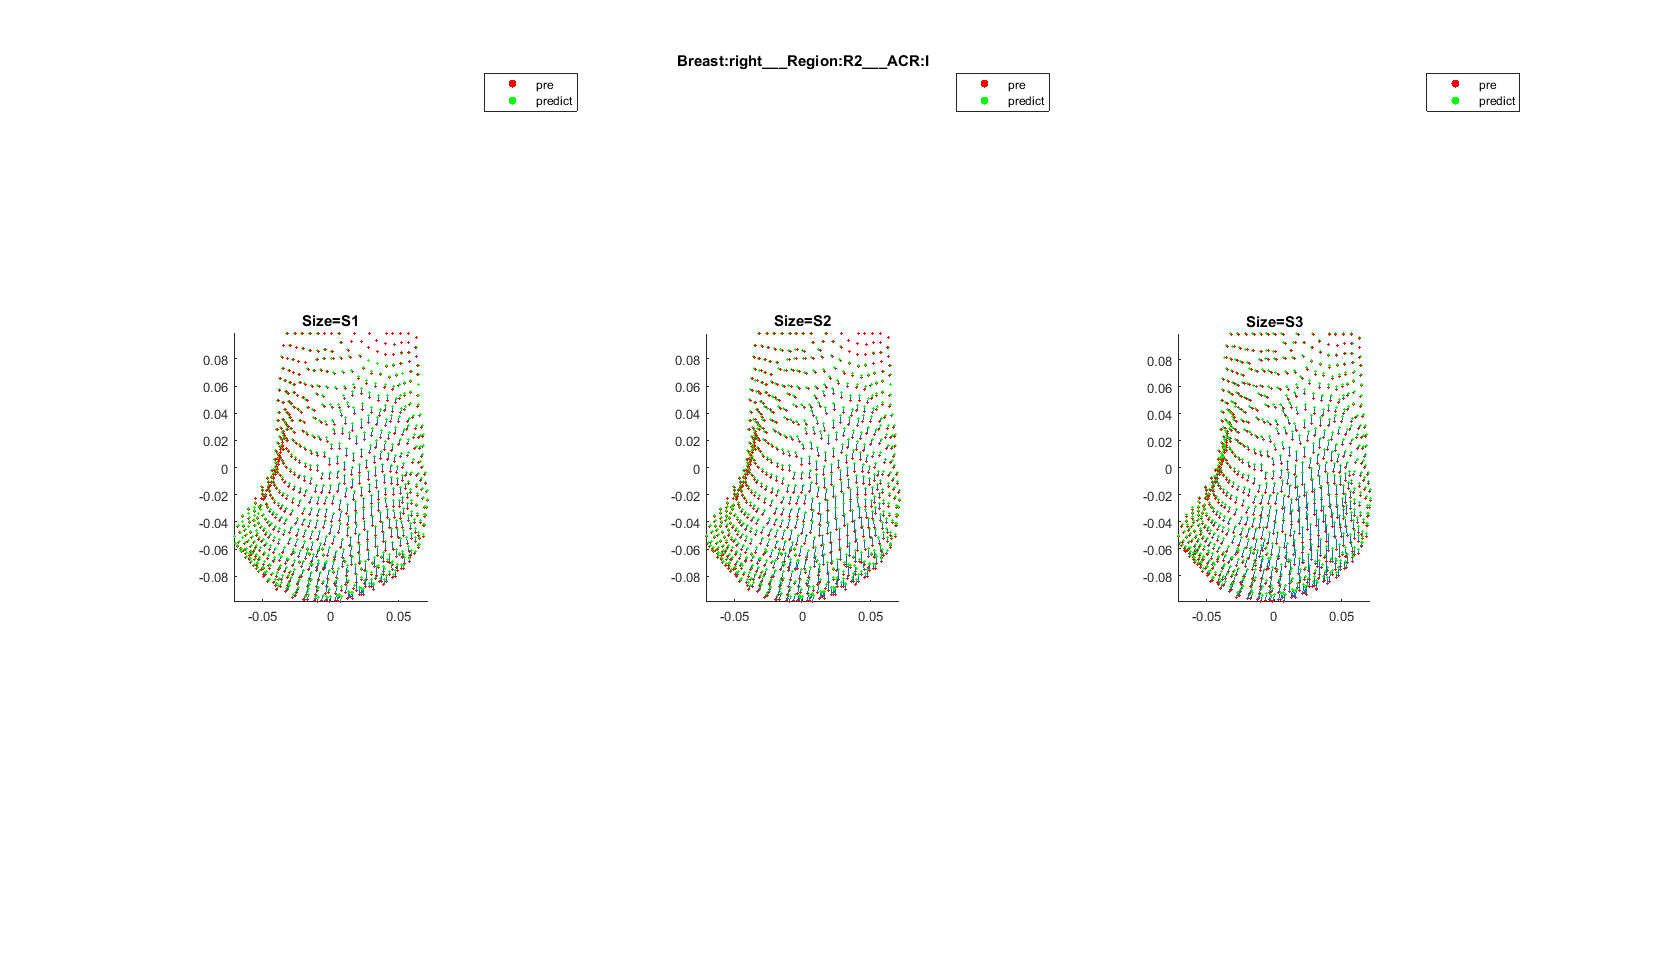
\includegraphics[width=1.2\textwidth]{size_analysis}
    \caption[Example of the impact of tumor's size on the breast's deformation]{Example of the impact of tumor's size on the breast's deformation}
    \label{fig:size_analysis}
  \end{center}
\end{figure}

\begin{figure}[!h]
\begin{center}
    \leavevmode
    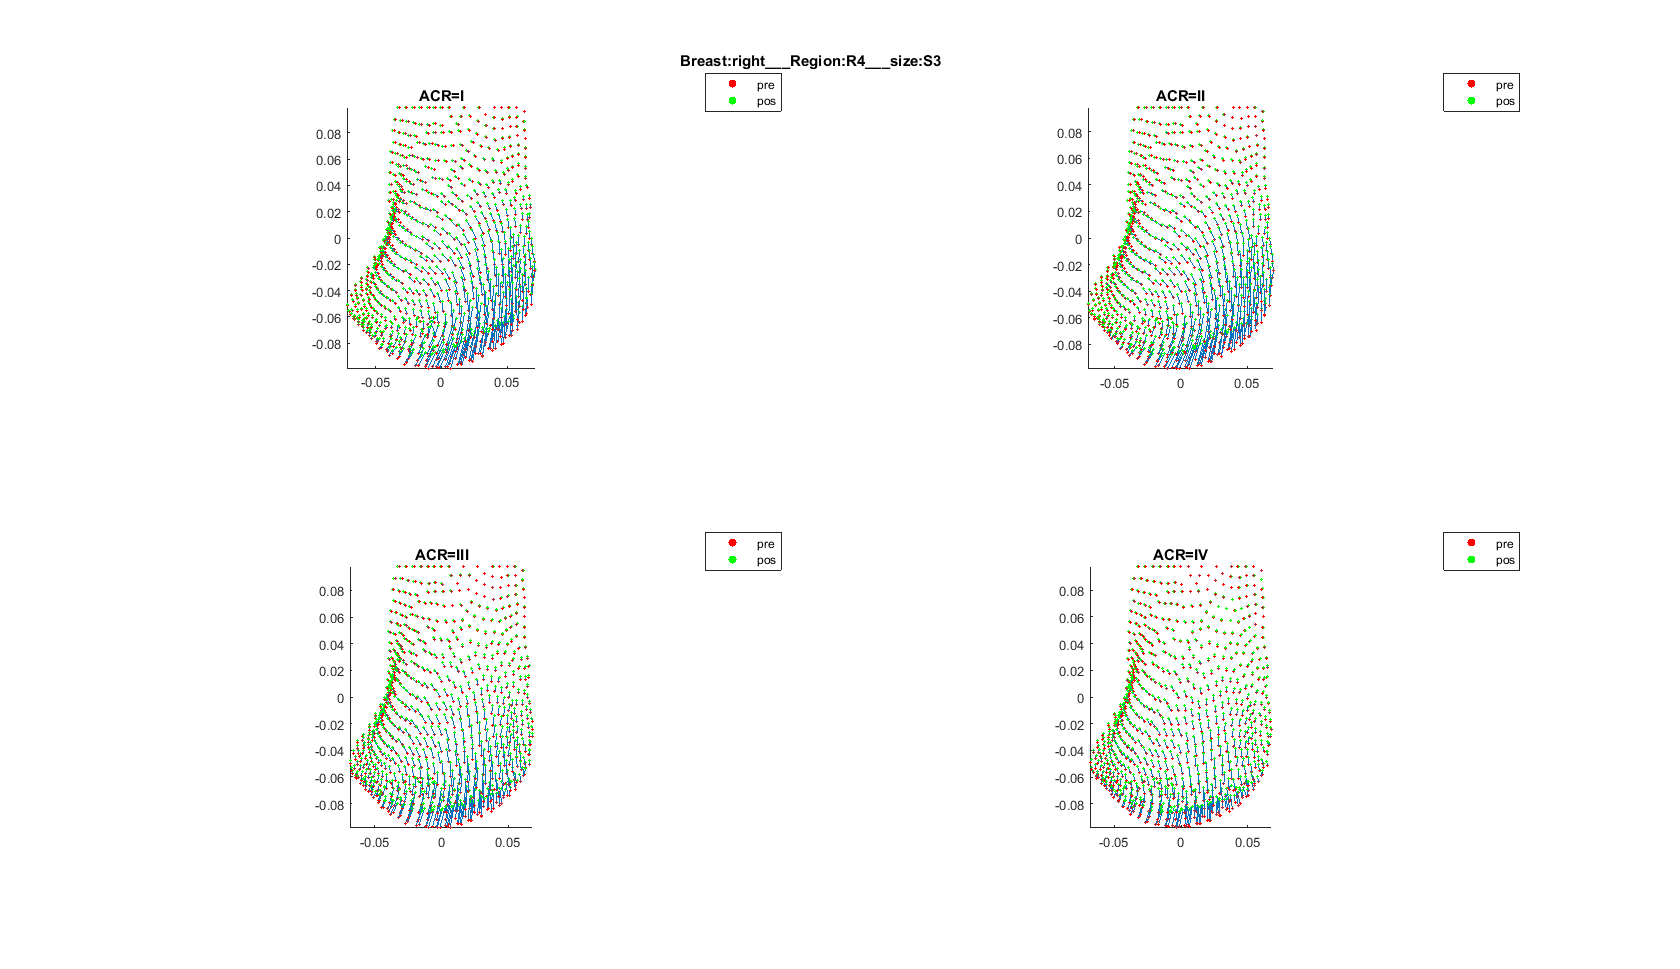
\includegraphics[width=1.2\textwidth]{acr_analysis}
    \caption[Example of the impact of breast density (ACR) on deformation]{Example of the impact of breast density (ACR) on deformation}
    \label{fig:acr_analysis}
  \end{center}
\end{figure}

Besides of these example, all the comparisons made and analyses in order to defer the impact of the clinical features on the breast deformation can be seen in appendix \ref{ap1:feat_analysis}.



\subsection{Feature Construction}

This analysis on clinical features also led to a few more conclusion about the deformation of the breast. Considering the new finding resultant from the feature analysis, some additional features were though to be helpful when trying to predict the new position of each point on the breast's point cloud. 
Despite of the findings regarding the clinical features, it was found is that the nearer surface points are to the tumour position, the more displacement they will suffer after the healing simulation. Having this in consideration, the euclidean distance and the difference for each axis, between the point itself and the tumor's center of mass, were computed and represented in both Cartesian and cylindrical coordinate. Being the cylindrical coordinates centred on the tumor's position.


\section{Model Design}

\subsection{Machine Learning Models}

As previously explained the intention of using ML (Machine Learning) Techniques is to predict the deformations caused by the BCS for the patients' breast. This prediction is carried out through the application of Regression Models which try to find a relation between the features training data, and the target values of the testing data. The target values will be the displacement of the points from the pre-surgical to the pos-surgical models of the breast.

\subsubsection{Feature Representation}

Despite of the tested scenario, the machine learning model will receive as input variables, the points of all the breasts in the training set. Each observation (as the input of the machine learning model) consists of a point from the pre-surgical model followed by several features regarding the characteristics of the breast. Initially, the training model will only have access to the points of the breast's surface, the front surface of the breast excluding the laterals, as seen in Figure \ref{fig:ML_input_pcl}. The models containing only the breast's surface that are going to be used contain an average of 629.33 point per model with a standard deviation of 106.68 points.

\begin{figure}[!h]
\centering
\begin{tabular}{cc}
\subfloat[Frontal view]{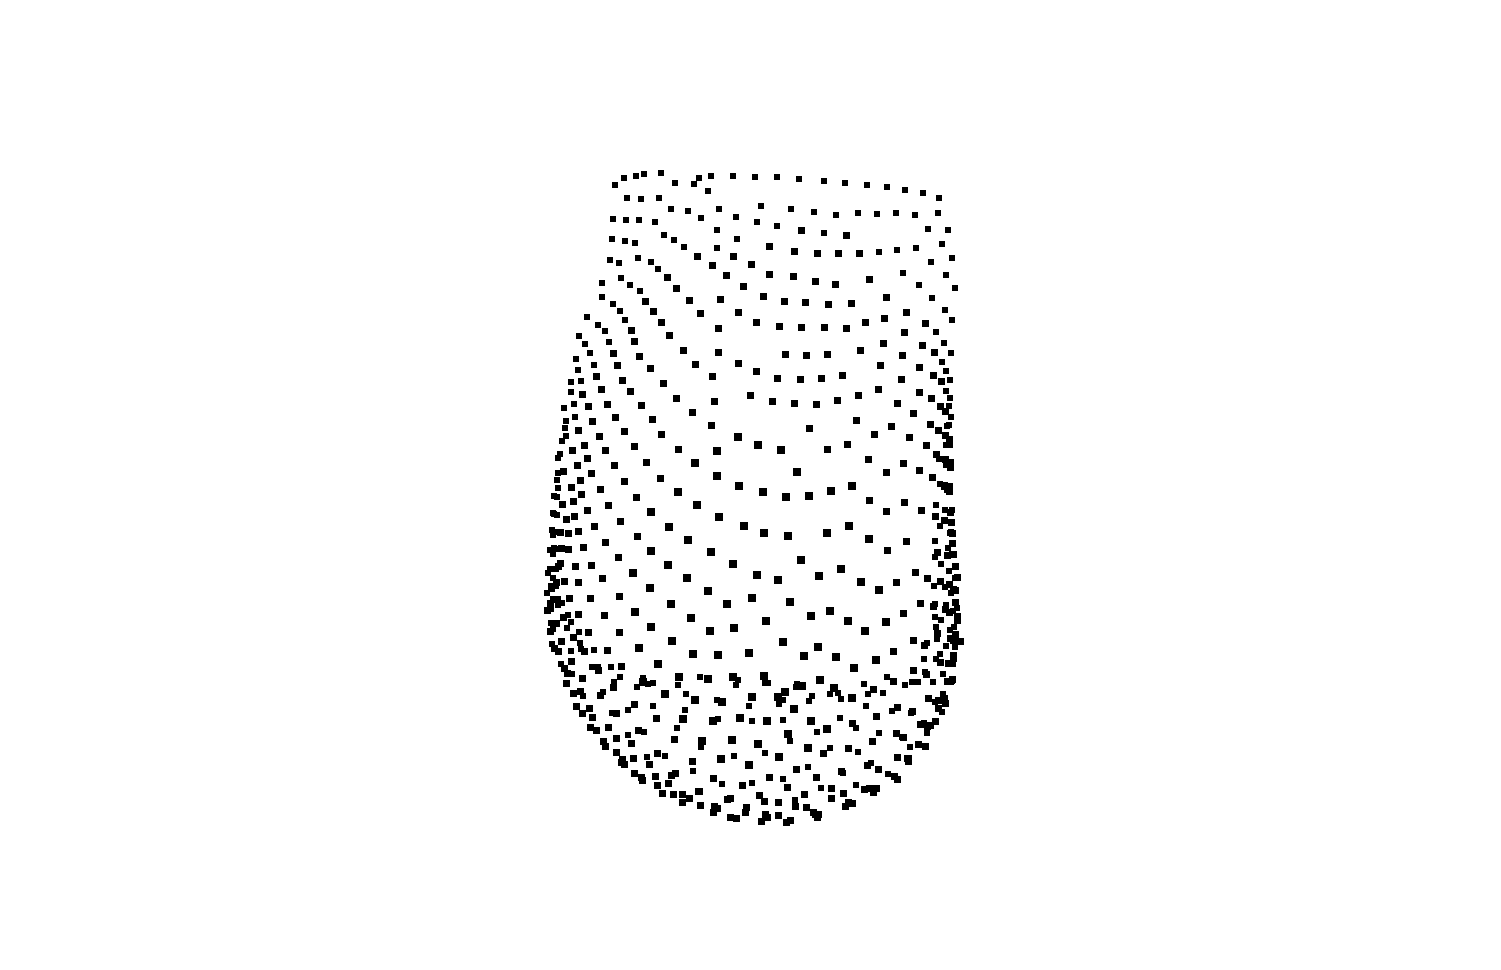
\includegraphics[width = 0.5\textwidth]{front}\label{fig:front_input}} &
\subfloat[Lateral view]{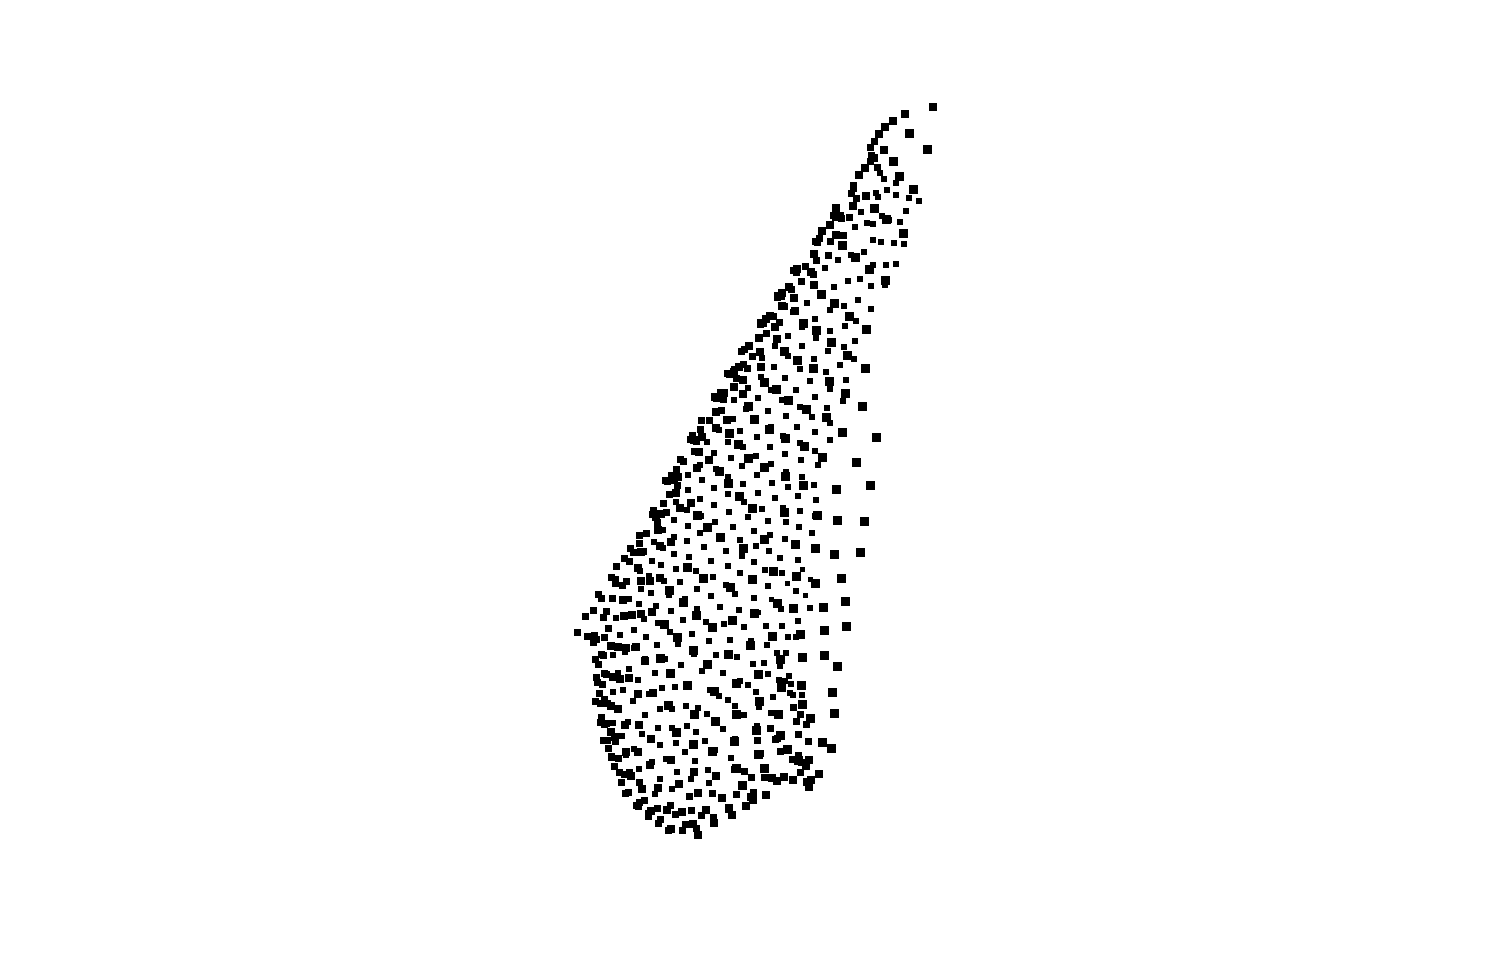
\includegraphics[width = 0.5\textwidth]{lateral}\label{fig:latearl_input}}
\end{tabular}
\caption[Example of breast point cloud to be used as ML input]{Example of breast point cloud to be used as ML input}
\label{fig:ML_input_pcl}
\end{figure}


The used features, when categorical as the laterality, the ACR of the breast, the tumor's region and tumor's size, will be represented as "dummy variables" \footnote{\url{http://imaging.mrc-cbu.cam.ac.uk/statswiki/FAQ/contint?action=AttachFile&do=get&target=int.pdf}}. Other features such as the point coordinates, breast volume, and distances will be represented as real values. 

The tumor's position defined by the breast's quadrant represents different quadrants of the breast according with the breasts laterality. For instance, while a region 4 (R4) on a left breast stands for the Lower left portion of the breast, the same region on the right breast refers to the Lower right portion. There are two possibilities in order to overcome this mismatch:
\begin{itemize}
\item Label the points according to the breast laterality, considering left and right points independent;
\item Reflect one of the breast over yOz plane or vice-versa as represented in Figure \ref{fig:reflection};
\end{itemize}

\begin{figure}[!h]
\centering
\begin{tabular}{cc}
\subfloat[left breast of a patient]{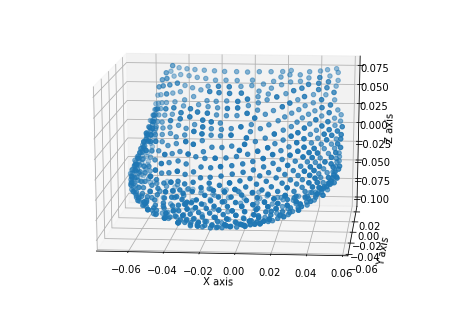
\includegraphics[width = 0.5\textwidth]{left2}\label{fig:reflection_left}} &
\subfloat[Reflection of the left breast of the patient]{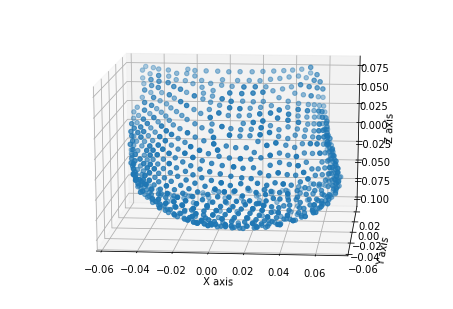
\includegraphics[width = 0.5\textwidth]{reflected2}\label{fig:reflection_reflected}}
\end{tabular}
\caption[Example of breast point cloud's reflection]{Example of breast point cloud's reflection}
\label{fig:reflection}
\end{figure}

Features like the breast laterality can be represented using categorical features or replaced by the breast's reflection. There are also features that will be represented in different ways, for instance the tumor's volume (real value of the breast's volume) and the tumor's size (categorical variable that represent the tumor as small, medium or large, regarding its size).

The Table \ref{tab:list_features} summarizes all the features that were used.

\begin{table}[!h]
%\label{tab:list_features}
\centering
\begin{tabular}{|p{16mm}|p{34mm}|p{15mm}|p{90mm}|}
\hline
\textbf{Feature}                                                     & \textbf{\begin{tabular}[c]{@{}l@{}}Feature \\ Description\end{tabular}}                                                                                                                                                                                                                                                             & \textbf{\begin{tabular}[c]{@{}l@{}}Variable\\ name\end{tabular}} & \textbf{\begin{tabular}[c]{@{}l@{}}Variable \\ Description\end{tabular}}                                                    \\ \hline \hline
\multirow{3}{*}{\begin{tabular}[c]{@{}l@{}}Point \\ coordinates\end{tabular}}                                   & \multirow{3}{*}{\begin{tabular}[c]{@{}l@{}} Point's representation \\ in a Cartesian \\ coordinate system\end{tabular}}                                                                                                                                                                                                   & x\_coord                                                            & coordinate of point in x axis                                                                                                  \\ \cline{3-4} 
                                                                     &                                                                                                                                                                                                                                                                                                                                    & y\_coord                                                            & coordinate of point in y axis                                                                                                  \\ \cline{3-4} 
                                                                     &                                                                                                                                                                                                                                                                                                                                    & z\_coord                                                            & coordinate of point in z axis                                                                                                  \\ \hline
\multirow{6}{*}{\begin{tabular}[c]{@{}l@{}} Distance's \\ projection \\ between \\ point and \\ tumor's \\ center of \\ mass\end{tabular}}                                   & \multirow{6}{*}{\begin{tabular}[c]{@{}l@{}}Distrance's projection \\ between the position \\ of the breast's point \\ and the tumor's center \\ of mass.\\ This difference can be \\ represented in a \\ Cartesian coordinate \\ system (variables \\ x\_dist, y\_dist and \\ z\_dist) or through \\ cylindrical coordinates \\ (variables theta, rho \\ and pol\_z)\end{tabular}} & x\_diff                                                             & distance's projection between the position of the point and the tumor's center of mass in a Cartesian coordinate system (x axis)          \\ \cline{3-4} 
                                                                     &                                                                                                                                                                                                                                                                                                                                    & y\_diff                                                             & distance's projection between the position of the point and the tumor's center of mass in a Cartesian coordinate system (y axis)          \\ \cline{3-4} 
                                                                     &                                                                                                                                                                                                                                                                                                                                    & z\_diff                                                             & distance's projection between the position of the point and the tumor's center of mass in a Cartesian coordinate system (z axis)          \\ \cline{3-4} 
                                                                     &                                                                                                                                                                                                                                                                                                                                    & theta                                                               & distance's projection between the position  of the point and the tumor's  center of mass in a cylindrical coordinate system (theta angle) \\ \cline{3-4} 
                                                                     &                                                                                                                                                                                                                                                                                                                                    & rho                                                                 & distance's projection between the position  of the point and the tumor's  center of mass in a cylindrical coordinate system (rho angle)   \\ \cline{3-4} 
                                                                     &                                                                                                                                                                                                                                                                                                                                    & pol\_z                                                              & distance's projection between the position  of the point and the tumor's  center of mass in a cylindrical coordinate system (z value)     \\ \hline
Distance                                                             & Euclidean distance between the point and the tumor's center                                                                                                                                                                                                                                                                & dist\_Tpt                                                           & Euclidean distance between the point and the tumor's center of mass                                                            \\ \hline
Breast's Volume                                                      & Pre-surgical breast's volume                                                                                                                                                                                                                                                                                          & b\_vol                                                              & Volume of the pre-surgical breast's model                                                                                      \\ \hline
\multirow{4}{*}{\begin{tabular}[c]{@{}l@{}}Tumor's \\ Size and \\ Volume\end{tabular}}                                & \multirow{4}{*}{\begin{tabular}[c]{@{}l@{}}Representation of the \\ tumor's volume, either \\ using the real value \\ or categorical variables\end{tabular}}                                                                                                                                                                                                                                            & t\_vol                                                              & Real value of the tumor's volume                                                                                               \\ \cline{3-4} 
                                                                     &                                                                                                                                                                                                                                                                                                                                    & t\_size\_a                                                          & Categorical variable to represent the tumor's size (small)                                                                           \\ \cline{3-4} 
                                                                     &                                                                                                                                                                                                                                                                                                                                    & t\_size\_b                                                          & Categorical variable to represent the tumor's size (medium)                                                                          \\ \cline{3-4} 
                                                                     &                                                                                                                                                                                                                                                                                                                                    & t\_size\_c                                                          & Categorical variable to represent the tumor's size (large)                                                                           \\ \hline
\multirow{2}{*}{\begin{tabular}[c]{@{}l@{}}Breast's \\ Laterality\end{tabular}}                                                               & \multirow{2}{*}{\begin{tabular}[c]{@{}l@{}}Representation of the \\ breast's laterality \\ (left or right breast)\end{tabular}}                                                                                                                                                                                                                                            & lat\_a                                                              & Categorical variable to represent the breast's laterality (Right Breast)                                                             \\ \cline{3-4} 
                                                                     &                                                                                                                                                                                                                                                                                                                                    & lat\_b                                                              & Categorical variable to represent the breast's laterality (Left Breast)                                                              \\ \hline
\multirow{4}{*}{\begin{tabular}[c]{@{}l@{}}Breast's \\ Density \\ (ACR)\end{tabular}}                                                           & \multirow{4}{*}{\begin{tabular}[c]{@{}l@{}}Representation of the \\ breast's density \\ using ACR\end{tabular}}                                                                                                                                                       & acr\_a                                                              & Categorical variable to represent the breast's density (ACR I)                                                                       \\ \cline{3-4} 
                                                                     &                                                                                                                                                                                                                                                                                                                                    & acr\_b                                                              & Categorical variable to represent the breast's density (ACR II)                                                                      \\ \cline{3-4} 
                                                                     &                                                                                                                                                                                                                                                                                                                                    & acr\_c                                                              & Categorical variable to represent the breast's density (ACR III)                                                                     \\ \cline{3-4} 
                                                                     &                                                                                                                                                                                                                                                                                                                                    & acr\_d                                                              & Categorical variable to represent the breast's density (ACR IV)                                                                      \\ \hline
\multirow{4}{*}{\begin{tabular}[c]{@{}l@{}}Tumor's \\ Location \\ (Region)\end{tabular}}                                                        & \multirow{4}{*}{\begin{tabular}[c]{@{}l@{}}Representation of the \\ tumor's location \\ regarding the breast's \\ quadrant\end{tabular}}                                                                                                                                                                                                                                            & reg\_a                                                              & Categorical variable to represent the tumor's located in R1                                                                          \\ \cline{3-4} 
                                                                     &                                                                                                                                                                                                                                                                                                                                    & reg\_b                                                              & Categorical variable to represent the tumor's located in R2                                                                          \\ \cline{3-4} 
                                                                     &                                                                                                                                                                                                                                                                                                                                    & reg\_c                                                              & Categorical variable to represent the tumor's located in R3                                                                          \\ \cline{3-4} 
                                                                     &                                                                                                                                                                                                                                                                                                                                    & reg\_d                                                              & Categorical variable to represent the tumor's located in R4                                                                          \\ \hline
\end{tabular}
\caption{List of Features}
\label{tab:list_features}
\end{table}

\subsubsection{Labels} \label{subsec:labels}

In order to obtain the shape of the breast after the BCS, the trained machine learning models predict the displacement of the points between the pre-surgical and pos-surgical models of the breast in each axis. This displacement is calculated by computing the difference in each axis between the pos-surgical point of the 3D model and the correspondent point in the pre-surgical 3D model. Through the feature analysis described in subsection \ref{subsec:feat_analysis}, it is evident that the axis where the points suffer a larger displacement is the \textit{z} axis.

\vspace{12mm}

Having the dataset ready with both the features and labels computed, the dataset was split into training and testing sets. This division was done in two different ways:
\begin{itemize}
\item Splitting the dataset by applying a Leave-one-out (LOO) methodology. The dataset is divided into 6 sets of data (one per each initial real patient, containing 48 cases each), and using alternately each one of the sets as test set and the remaining 5 sets as training set;
\item Randomly split the 288 cases of the complete dataset using 1/6 of the cases as testing set and the remaining cases (5/6) as training set.
\end{itemize}

Regarding the validation set, the models use 10-fold cross validation. As expected and as can be seen in chapter \ref{chap:results}, randomly splitting the data leads to much better although misleading results than the other approach for the splitting of the dataset into training and testing sets. This is justified by the similarity of the breast within the training and the testing set, since both of them are simulations of the same initial patient despite of the different clinical features. The use of this biased testing set allowed the representation of a best case scenario for the prediction of the breast's deformation.

\subsubsection{Machine Learning Algorithms} \label{subsec:implementation}

In order to train the machine learning models that will be used to predict the displacement of the pre-surgical model to the pos-surgical, the following machine learning algorithms were used in order to solve this regression problem. 

\begin{itemize}
\item Multilayer Perceptron (MLP)

MLP, also known as feedforward neural networks (FFNN) is a type of Artificial Neural Networks widely used when targetting clinical medical issues \cite{Finne2000}. They consist of a set of nodes connected by edges that simulate the behaviour of neurons of the human brain. \cite{Nygren2016}

The node is responsible to compute the weighted sum of the inputs  $ z = \sum_{j=1}^{m} w_j x_j $ and to apply an activation function $ y = \varphi (z+b) $, where $x_j$ is the input for input link $j$ , $w_j$ the weight for the same input, $y$ the output of the neuron, $b$ the optimal bias parameters added to the input and $\varphi$ is an activation function.

An example of a MLP is represented in Figure \ref{fig:NN} consisting of multiple layers of fully connected neurons. The represented layers differ in three types:
\begin{itemize}
\item Input layers - only transport all the inputs to the next layer; 
\item Hidden layers - adjust the weighed sum of the inputs, compute the activation function and output the values to the next layer;
\item Output layers - perform the same computations that hidden layers do and output the values as the network's result.
\end{itemize}

\begin{figure}[!h]
\begin{center}
    \leavevmode
    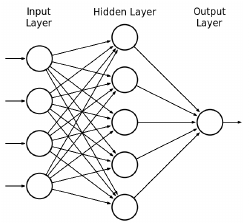
\includegraphics[width=0.5\textwidth]{NN}
    \caption[Representation of a MLP]{Representation of a MLP \cite{Ortiz2016}}
    \label{fig:NN}
  \end{center}
\end{figure}

The number of neurons highly depends on the amount and properties of the training data, as well as the number of hidden layers. And the Learning rate impacts the step used to adjust the inputs' weight.

\item Random Forest (RF)

The Random Forest (RF) algorithm is based on using multiple decisions trees, mitigating the negative aspects of decision trees by ignoring some of the input properties and increasing the performance of the algorithm.
Each decision tree on the RF system, only consider a random subset of the input data, and consider a limited number of features smaller than the number of total features. The output of the several decision trees is then averaged and used as output of the RF \cite{Nygren2016}.

The splitting criteria for regression problems in RF algorithms to divide the root or leaf into more leafs is calculate through $ RSS = \sum_{LEFT} (Y_i - Y_{L}^{*})^{2} + \sum_{RIGHT} (Y_i - Y_{R}^{*})^{2}$, where $RSS$ stands for Residual sum of the squares, $Y_i$ stands for the current node and $Y_L^{*}$ and $Y_R^{*}$ stands for the mean value of \textit{y} for both the left and right nodes, respectively \cite{Cutler2013}.

Figure \ref{fig:RF} presents an example of a decision tree regression result.

\begin{figure}[!h]
\begin{center}
    \leavevmode
    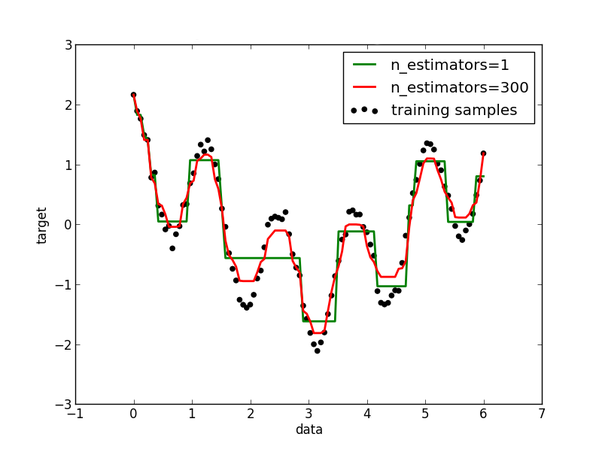
\includegraphics[width=0.7\textwidth]{RF}
    \caption[Example of a RF result]{Example of a RF result. Comparison of results of a RF with only a decision tree (green) and a RF with 300 decision trees (red). The scatter point represent the data used to train the RF. \protect\footnotemark}
    \label{fig:RF}
  \end{center}
\end{figure}
\footnotetext{\url{https://www.quora.com/How-does-random-forest-work-for-regression-1}}

This type of algorithm has as great advantage not requiring a prior feature section, and despite of being promising, it is only capable of predicting the regression of a variable. In this case, in order to predict the total displacement of the point between models, three individual training models are required, one for each Cartesian axis.

\item Multioutput Regression (MOR)

Multioutput regression also known as multi-variate or multi-target regression, has been used on multiple applications across several fields of study \cite{Borchani}. This ML approach allows the prediction of several output variables for each entry of the model. \footnote{\label{mor} \url{http://scikit-learn.org/stable/modules/multiclass.html\#multiclass}} Other advantage of this type of approach is that the produced models are, generally, simpler and more computational efficient.

One of the several multioutput regression method consists on the adaptation of other ML algorithms such as RF in order to allow them to predict several output variables. This type of multioutput regressors requires the identification of the dependencies among the target variables. When compared to regular RF, multi-target regression trees usually require a smaller number of trees for all the variables, and allow a more informed understanding of the dependencies among the several target variables of the model \cite{Borchani}.


\end{itemize}


\subsubsection{Implementation}

As already stated, the presented algorithms were implemented aiming to predict the displacement between the pre-surgical and the pos-surgical models. The displacement for \textit{x} axis, \textit{y} axis and \textit{z} axis are respectively represented as \textit{$\partial$x}, \textit{$\partial$y} and \textit{$\partial$z}.

The 3 previously described machine learning algorithms were implemented using 10 fold cross validation in order to automatically tune each algorithm parameters leading the algorithm to achieve the minimum root mean squared error of the model. The 3 algorithms were used to train both of the splits of the dataset (LOO and the random split using 1/6 of the data as the test set).

A short feature selection was done to understand which features should be used as well as their representations. The feature selection was done recurring to recursive feature elimination \footnote{\url{https://topepo.github.io/caret/recursive-feature-elimination.html}}, and then a trial was done using MLP. Regarding the training of RF and MOR, this study was not necessary since both algorithms support a built-in feature selection method that measures the feature's importance \footnote{\url{https://topepo.github.io/caret/feature-selection-overview.html}}. The last two algorithms led to the training of random forest models for each axis (\textit{x}, \textit{y} and \textit{z} axis); and the training of multi output regressor models, considering the \textit{$\partial$z}, \textit{$\partial$y}, \textit{$\partial$x} as labels; \textit{$\partial$y} and \textit{$\partial$x} as labels; and \textit{$\partial$x} and \textit{$\partial$y} as labels.

In order to implement the random forests and multi-layer perceptron algorithms a R package named caret \footnote{\label{caret} \url{https://cran.r-project.org/web/packages/caret/caret.pdf}} was used. Multi-output regressor was implemented with a R package called randomForestSRC package \footnote{\label{rfsrc} \url{https://cran.r-project.org/web/packages/randomForestSRC/randomForestSRC.pdf}}.

\subsection{Naive Model} \label{sub_sec:naive_method_explanation}

In order to understand the impact of ML techniques to predict the deformation, a naive method was created to generate the shape of the breast using common sense and conclusion arising from the feature analysis presented in section \ref{subsec:feat_analysis}.

Two alternatives for the naive method were developed, where the displacement between the pre-surgical and pos-surgical models of the breast were computed as follows:
\begin{enumerate}
\item The first alternative consisted on calculating the average displacement of the points on each geometric quadrant of the breast. The average displacement of each quadrant is calculated based on the mean displacement of the points on the same quadrant in similar breasts. These similar breast concerns all the breasts on the dataset, that were generated from a different initial patient, with the same breast properties: breast's laterality and density and the same tumor's properties.

For instance, if the breast that is under the naive method has the tumor located in region 2, the average displacement for the correspondent quadrant will be calculated based on the other patients with the tumor on the same region, the same tumor's size and the same breast's laterality and density. For the regions were the tumor is not located, the average displacement will be calculated based on the breasts of the dataset, that do not have the tumor located on that region and with the same breast's properties and tumor's size. Therefore, the quadrants are defined based on the geometric center of the breast.

In spite of calculating an average displacement for the all quadrants of the breast, only a portion of that displacement is applied to the pre-surgical model. Each quadrant was divided into 3 stacks across the z axis, and a portion or the total displacement was applied based on how much the points on that region would normally move. The stack division is done equally, however the portion of the applied displacement on the \textit{x}, \textit{y} and \textit{z} axis differs according to the quadrants (lower or upper quadrant).

\item  The second approach of the naive method, is divided into two steps. In the first step, and similar with what happens on the first approach, the breast is divided into quadrants, however considering the nipple's position but not the geometric center of the breast. In the second step, and taking into consideration all breasts in the dataset, the average displacement of points is calculated for each quadrant of the breast. When considering the quadrant where the tumor is located, the points below the tumor are updated by subtracting their height from the mean displacement previously calculated; When considering the not affected quadrants (without the tumor located on them), the points' position is updated. Calculating the ratio between the average displacement of the non-affected quadrants and the distance from the point to the tumor's center of mass, will give a value that, when subtracted from the point's previous position will result on the new position of the point. The computed displacements are also multiplied by the breasts' ACR using a factor of 1.2, due to the relation between the breast's ACR and the breast's deformation.

\end{enumerate}

\section{Results Validation}

Despite of the use of cross validation and the parameter tuning used on the implementation of the machine learning models that tried to decrease the root mean squared error between the predicted data and the given labels, the obtained results were evaluated using some evaluation metrics. As previously described, the given machine learning models had as goal to predict the displacement of each point in the breast's 3D model in one or more axis. Summing the predicted values to the correspondent point of the pre-surgical breast's model, ideally would produce the pos-surgical model of the breast.

\subsection{Evaluation Metrics}

There were considered two types of evaluation metrics:
\begin{itemize}
\item Visual metrics;

The visual metrics consists of visual comparison between pre-surgical, pos-surgical and predicted models of the breast. This evaluation allows to easily gather some conclusion regarding the models performance.

\item Distance metrics.

The distance metrics allows to obtain a more accurate perception of the model's performance.
\end{itemize}

\subsubsection{Distance metrics}

The distances computed for evaluating the models consider both local and global distances: while, the local distance, compare the models point by point, the global distances is measured in both directions comparing each point of a model to another breast's model and a breast's model to a point of another model. Regarding the local metric, the distances to be measured are the one between the predicted model and the pos-surgical model (\textit{predicted to pos}); the distance between the pre-surgical to the pos-surgical models (\textit{pre to pos}); and the distance between the predicted model and the pre-surgical model (\textit{predicted to pre}). Regarding the global metric, the same distances will be measures, however in both directions: \textit{predicted to pos}; \textit{pos to predicted}; \textit{pre to pos}; \textit{pos to pre}; \textit{predicted to pre}; and \textit{pre to predicted}. 

On either case the following values are computed:
\begin{itemize}
\item Mean of Euclidean distance;
\item Standard Deviation of the Euclidean distance;
\item Hausdorff distance (maximum of the euclidean distances).
\end{itemize}

These values are calculated considering the 3 coordinates of each point (3D), or only the point's projection in one of the Cartesian coordinate system axis(1D).


\section{Summary}

The present chapter, described the complete process that was followed in order to predict the deformation caused by BCS. Initially the dataset preparation was described, and some additional information was given, in order to understand its construction. Then a analysis of the clinical features was also detailed and results presented in the chapter. Thereafter the models used in order to predict the breast deformations were explained. Regarding the introduced machine learning techniques, a short background of the regression models was provided and all the relevant information about their implementation and application is outlined. At last, the evaluation metrics were also described.

All the results and further conclusion arising from the detailed methodology are explored in chapter \ref{chap:results}. 




\chapter{Results and Discussion}\label{chap:results}

\section*{}

This chapter intends to present the results for both the several performed machine learning runs using different algorithms and different features as well as different combinations of features and the naive implementations. By analysing the results using visual cues and the evaluation metrics previously defined in chapter \ref{chap:method}, the upcoming findings suggest if the machine learning techniques are correctly predicting the breast deformation. The results will also be further analysed in order to understand on which regions of the breast, the prediction is more inaccurate in terms of distance between the predicted and the real data. 

The current chapter is divided into 3 sections, being the first two, section \ref{sec:naive_results} and section \ref{sec:ml_results}, used to shown the visual and evaluation metrics' results for the naive methods and the machine learning models respectively. Section \ref{sec:heatmap} will present the regions of the breast where the predictions are more inaccurate.
All the results and intermediary conclusions will be used to draw the final conclusions present in chapter \ref{chap:concl}.

\section{Naive Method Results} \label{sec:naive_results}

As described before, two different naive methods approaches were tried in order to predicted the deformation caused by BCS. The implementation of this approach has as goal, understanding the improvement provided by the use of machine learning techniques instead of using methods based on common sense and the findings resultant from the feature analysis in section \ref{subsec:feat_analysis}.

Table \ref{tab:naive1} shows the global evaluation metrics for the the naive method described in section \ref{sub_sec:naive_method_explanation} that uses the geometric center of the breast in order to divide it into quadrants. Table \ref{tab:naive1_local} represents the local evaluation metrics in the same conditions. As shown the prediction made by the naive method leads to the movement, not very significant, of the breast's. This effect can be visualized in Figure \ref{fig:naive1}. Using this method leads to an over prediction of the displacement in cases similar to the one represented in Figure \ref{fig:naive1_left}, where the the breast suffers a minor deformation caused by the BCS and to an under prediction of the displacement in cases similar to the one represented in Figure \ref{fig:naive1_right}, where the breast's deformation caused by the BCS is more severe. 

% Please add the following required packages to your document preamble:
% \usepackage{multirow}
\begin{table}[!htb]
\centering
\begin{tabular}{lll|l|l|l|l|l|l|}
\cline{4-9}
                                                   &                                                                                                             &                                                                       & \textbf{\begin{tabular}[c]{@{}l@{}}predicted\\  to pos\end{tabular}} & \textbf{\begin{tabular}[c]{@{}l@{}}pos to \\ predicted\end{tabular}} & \textbf{pre to pos} & \textbf{pos to pre} & \textbf{\begin{tabular}[c]{@{}l@{}}predicted\\  to pre\end{tabular}} & \textbf{\begin{tabular}[c]{@{}l@{}}pre to \\ predicted\end{tabular}} \\ \hline
\multicolumn{1}{|l|}{\multirow{3}{*}{\textbf{3D}}} & \multicolumn{1}{l|}{\multirow{2}{*}{\textbf{\begin{tabular}[c]{@{}l@{}}Euclidean\\ Distance\end{tabular}}}} & \textbf{Mean}                                                         & 1.731                                                                & 1.725                                                                & 1.758               & 1.731               & 1.420                                                                & 1.421                                                                \\ \cline{3-9} 
\multicolumn{1}{|l|}{}                             & \multicolumn{1}{l|}{}                                                                                       & \textbf{\begin{tabular}[c]{@{}l@{}}Standard\\ Deviation\end{tabular}} & 1.130                                                                & 1.113                                                                & 1.333               & 1.277               & 1.064                                                                & 1.394                                                                \\ \cline{2-9} 
\multicolumn{1}{|l|}{}                             & \multicolumn{2}{l|}{\textbf{\begin{tabular}[c]{@{}l@{}}Hausdorff Distance\end{tabular}}}                                                                                          & 5.563                                                                & 5.539                                                                & 6.513               & 6.317               & 2.939                                                                & 6.452                                                                \\ \hline
\multicolumn{1}{|l|}{\multirow{3}{*}{\textbf{1D}}} & \multicolumn{1}{l|}{\multirow{2}{*}{\textbf{\begin{tabular}[c]{@{}l@{}}Euclidean\\ Distance\end{tabular}}}} & \textbf{Mean}                                                         & 0.141                                                                & 0.123                                                                & 0.160               & 0.110               & 0.113                                                                & 0.083                                                                \\ \cline{3-9} 
\multicolumn{1}{|l|}{}                             & \multicolumn{1}{l|}{}                                                                                       & \textbf{\begin{tabular}[c]{@{}l@{}}Standard\\ Deviation\end{tabular}} & 0.210                                                                & 0.145                                                                & 0.346               & 0.110               & 0.142                                                                & 0.243                                                                \\ \cline{2-9} 
\multicolumn{1}{|l|}{}                             & \multicolumn{2}{l|}{\textbf{\begin{tabular}[c]{@{}l@{}}Hausdorff Distance\end{tabular}}}                                                                                          & 1.631                                                                & 1.203                                                                & 3.168               & 0.704               & 0.787                                                                & 3.325                                                                \\ \hline
\end{tabular}
\caption{Global Evaluation Metrics for the first approach of the naive method}
\label{tab:naive1}
\end{table}

\begin{table}[!htb]
\centering
%\label{naive1_local}
\begin{tabular}{lll|l|l|l|}
\cline{4-6}
                                                   &                                                                                                             &                                                                       & \textbf{\begin{tabular}[c]{@{}l@{}}predicted\\  to pos\end{tabular}} & \textbf{pre to pos} & \textbf{\begin{tabular}[c]{@{}l@{}}predicted\\  to pre\end{tabular}} \\ \hline
\multicolumn{1}{|l|}{\multirow{3}{*}{\textbf{3D}}} & \multicolumn{1}{l|}{\multirow{2}{*}{\textbf{\begin{tabular}[c]{@{}l@{}}Euclidean\\ Distance\end{tabular}}}} & \textbf{Mean}                                                         & 1.980                                                                & 2.206               & 1.426                                                                \\ \cline{3-6} 
\multicolumn{1}{|l|}{}                             & \multicolumn{1}{l|}{}                                                                                       & \textbf{\begin{tabular}[c]{@{}l@{}}Standard\\ Deviation\end{tabular}} & 1.503                                                                & 1.920               & 1.070                                                                \\ \cline{2-6} 
\multicolumn{1}{|l|}{}                             & \multicolumn{2}{l|}{\textbf{Hausdorff Distance}}                                                                                                                                    & 7.000                                                                & 8.410               & 2.939                                                                \\ \hline
\multicolumn{1}{|l|}{\multirow{3}{*}{\textbf{1D}}} & \multicolumn{1}{l|}{\multirow{2}{*}{\textbf{\begin{tabular}[c]{@{}l@{}}Euclidean\\ Distance\end{tabular}}}} & \textbf{Mean}                                                         & 1.601                                                                & 1.904               & 1.397                                                                \\ \cline{3-6} 
\multicolumn{1}{|l|}{}                             & \multicolumn{1}{l|}{}                                                                                       & \textbf{\begin{tabular}[c]{@{}l@{}}Standard\\ Deviation\end{tabular}} & 1.530                                                                & 1.929               & 1.085                                                                \\ \cline{2-6} 
\multicolumn{1}{|l|}{}                             & \multicolumn{2}{l|}{\textbf{Hausdorff Distance}}                                                                                                                                    & 6.635                                                                & 8.092               & 2.926                                                                \\ \hline
\end{tabular}
\caption{Local Evaluation Metrics for the first approach of the naive method}
\label{tab:naive1_local}
\end{table}

\begin{figure}[!htb]
\centering
\begin{tabular}{cc}
\subfloat[Example of a breast with a less deformation caused by BCS]{\includegraphics[width = 0.315\textwidth]{naive1_102_cut}\label{fig:naive1_left}} &
\subfloat[Example of a breast with a more noticeable deformation caused by BCS]{\includegraphics[width = 0.3\textwidth]{naive1_200_cut}\label{fig:naive1_right}}
\end{tabular}
\caption[Comparison between pre-surgical, pos-surgical and predicted through a naive method breast's models]{Comparison between pre-surgical, pos-surgical and predicted through a naive method breast's models. The pre-surgical model is displayed in blue; the pos-surgical models displayed in green, and the naive predicted model displayed in orange.}
\label{fig:naive1}
\end{figure}

The global and local evaluation metrics for the second implementation of the naive method also described in section \ref{sub_sec:naive_method_explanation} are represented respectively in Table \ref{tab:naive2} and Table \ref{tab:naive2_local}. Despite of the improvement on the evaluation metrics, the same effect represent in Figure \ref{fig:naive1} still occurs as shown in Figure \ref{fig:naive2}.

\begin{table}[!htb]
\centering
%\label{tab:naive2}
\begin{tabular}{lll|l|l|l|l|l|l|}
\cline{4-9}
                                                   &                                                                                                             &                                                                       & \textbf{\begin{tabular}[c]{@{}l@{}}predicted\\  to pos\end{tabular}} & \textbf{\begin{tabular}[c]{@{}l@{}}pos to \\ predicted\end{tabular}} & \textbf{pre to pos} & \textbf{pos to pre} & \textbf{\begin{tabular}[c]{@{}l@{}}predicted\\  to pre\end{tabular}} & \textbf{\begin{tabular}[c]{@{}l@{}}pre to \\ predicted\end{tabular}} \\ \hline
\multicolumn{1}{|l|}{\multirow{3}{*}{\textbf{3D}}} & \multicolumn{1}{l|}{\multirow{2}{*}{\textbf{\begin{tabular}[c]{@{}l@{}}Euclidean\\ Distance\end{tabular}}}} & \textbf{Mean}                                                         & 1.523                                                                & 1.503                                                                & 1.758               & 1.731               & 1.414                                                                & 1.415                                                                \\ \cline{3-9} 
\multicolumn{1}{|l|}{}                             & \multicolumn{1}{l|}{}                                                                                       & \textbf{\begin{tabular}[c]{@{}l@{}}Standard\\ Deviation\end{tabular}} & 1.194                                                                & 1.129                                                                & 1.333               & 1.277               & 1.067                                                                & 1.069                                                                \\ \cline{2-9} 
\multicolumn{1}{|l|}{}                             & \multicolumn{2}{l|}{\textbf{Hausdorff Distance}}                                                                                                                                    & 5.327                                                                & 5.137                                                                & 6.513               & 6.317               & 2.939                                                                & 2.939                                                                \\ \hline
\multicolumn{1}{|l|}{\multirow{3}{*}{\textbf{1D}}} & \multicolumn{1}{l|}{\multirow{2}{*}{\textbf{\begin{tabular}[c]{@{}l@{}}Euclidean\\ Distance\end{tabular}}}} & \textbf{Mean}                                                         & 0.127                                                                & 0.113                                                                & 0.160               & 0.110               & 0.073                                                                & 0.090                                                                \\ \cline{3-9} 
\multicolumn{1}{|l|}{}                             & \multicolumn{1}{l|}{}                                                                                       & \textbf{\begin{tabular}[c]{@{}l@{}}Standard\\ Deviation\end{tabular}} & 0.194                                                                & 0.120                                                                & 0.346               & 0.110               & 0.101                                                                & 0.193                                                                \\ \cline{2-9} 
\multicolumn{1}{|l|}{}                             & \multicolumn{2}{l|}{\textbf{Hausdorff Distance}}                                                                                                                                    & 1.685                                                                & 0.851                                                                & 3.168               & 0.704               & 0.618                                                                & 2.091                                                                \\ \hline
\end{tabular}
\caption{Global Evaluation Metrics for the second approach of the naive method}
\label{tab:naive2}
\end{table}

\begin{table}[!htb]
\centering
%\label{tab:naive2_local}
\begin{tabular}{lll|l|l|l|}
\cline{4-6}
                                                   &                                                                                                             &                                                                       & \textbf{\begin{tabular}[c]{@{}l@{}}predicted\\  to pos\end{tabular}} & \textbf{pre to pos} & \textbf{\begin{tabular}[c]{@{}l@{}}predicted\\  to pre\end{tabular}} \\ \hline
\multicolumn{1}{|l|}{\multirow{3}{*}{\textbf{3D}}} & \multicolumn{1}{l|}{\multirow{2}{*}{\textbf{\begin{tabular}[c]{@{}l@{}}Euclidean\\ Distance\end{tabular}}}} & \textbf{Mean}                                                         & 1.634                                                                & 2.206               & 1.723                                                                \\ \cline{3-6} 
\multicolumn{1}{|l|}{}                             & \multicolumn{1}{l|}{}                                                                                       & \textbf{\begin{tabular}[c]{@{}l@{}}Standard\\ Deviation\end{tabular}} & 1.497                                                                & 1.920               & 1.124                                                                \\ \cline{2-6} 
\multicolumn{1}{|l|}{}                             & \multicolumn{2}{l|}{\textbf{Hausdorff Distance}}                                                                                                                                    & 5.763                                                                & 8.410               & 3.152                                                                \\ \hline
\multicolumn{1}{|l|}{\multirow{3}{*}{\textbf{1D}}} & \multicolumn{1}{l|}{\multirow{2}{*}{\textbf{\begin{tabular}[c]{@{}l@{}}Euclidean\\ Distance\end{tabular}}}} & \textbf{Mean}                                                         & 1.231                                                                & 1.904               & 1.397                                                                \\ \cline{3-6} 
\multicolumn{1}{|l|}{}                             & \multicolumn{1}{l|}{}                                                                                       & \textbf{\begin{tabular}[c]{@{}l@{}}Standard\\ Deviation\end{tabular}} & 1.055                                                                & 1.929               & 0.924                                                                \\ \cline{2-6} 
\multicolumn{1}{|l|}{}                             & \multicolumn{2}{l|}{\textbf{Hausdorff Distance}}                                                                                                                                    & 5.174                                                                & 8.092               & 5.191                                                                \\ \hline
\end{tabular}
\caption{Local Evaluation Metrics for the second approach of the naive method}
\label{tab:naive2_local}
\end{table}

\begin{figure}[!htb]
\centering
\begin{tabular}{cc}
\subfloat[Example of a breast with a lesser deformation caused by BCS]{\includegraphics[width = 0.315\textwidth]{naive2_102_cut}\label{fig:naive2_left}} &
\subfloat[Example of a breast with a more noticeable deformation caused by BCS]{\includegraphics[width = 0.3\textwidth]{naive2_200_cut}\label{fig:naive2_right}}
\end{tabular}
\caption[Comparison between pre-surgical, pos-surgical and predicted breast's models through the second implementation of a naive method ]{Comparison between pre-surgical, pos-surgical and predicted through a naive method breast's models. The pre-surgical model is displayed in blue; the pos-surgical model is displayed in green, and the naive predicted model is displayed in orange.}
\label{fig:naive2}
\end{figure}

\section{Machine Learning Results} \label{sec:ml_results}

The different algorithms described in section \ref{subsec:implementation} were used to train the several prediction models.

The following sections present the results for each ML algorithm in order to understand what led to a better prediction, as well as the features and labels that should be used on each case.

\subsection{Random Forest Results} \label{subsec:rf_results}

In order to predict the displacement of the breast's surface points using RF, three different models were built: one for each axis. Despite of the 3 models, the evaluation was done considering the simultaneous outcome of the three models.

On an initial approach, only considering the surface points in order to train the models, features such the points' coordinates, the distance from the point to the tumor's center of mass, the breast's volume, the tumor's volume and the remaining clinical features as dummy variables. as the points were considered. Another trials were carried out, where the features were represented differently or even omitted. On one of those trials, instead of using the breast's laterality as a categorical variable, the right breast were reflected and considered left breast, leading to worse results in terms of a more inaccurate displacement prediction.

Both global and local evaluation metrics are respectively displayed in Table \ref{tab:rf_loo_g} and Table \ref{tab:rf_loo_l} for the LOO train/test splitting and in Table \ref{tab:rf_biased_g} and Table \ref{tab:rf_biased_l} for the biased train/test split. The biased split (as described in section \ref{subsec:labels}) was constructed by randomly splitting the dataset cases into train and test sets. Since all the cases in the dataset were generated from 6 initial real patients, there is a great probability of a case in the test set having a very similar cases on the training set. By using this is possible to represent an ideal situation of the breast's deformation prediction and understand the results of the best case scenario of the prediction model.


\begin{table}[!htb]
\centering
\begin{tabular}{lll|l|l|l|l|l|l|}
\cline{4-9}
                                                   &                                                                                                             &                                                                       & \textbf{\begin{tabular}[c]{@{}l@{}}predicted\\  to pos\end{tabular}} & \textbf{\begin{tabular}[c]{@{}l@{}}pos to \\ predicted\end{tabular}} & \textbf{pre to pos} & \textbf{pos to pre} & \textbf{\begin{tabular}[c]{@{}l@{}}predicted\\  to pre\end{tabular}} & \textbf{\begin{tabular}[c]{@{}l@{}}pre to \\ predicted\end{tabular}} \\ \hline
\multicolumn{1}{|l|}{\multirow{3}{*}{\textbf{3D}}} & \multicolumn{1}{l|}{\multirow{2}{*}{\textbf{\begin{tabular}[c]{@{}l@{}}Euclidean\\ Distance\end{tabular}}}} & \textbf{Mean}                                                         & 1.103                                                                & 1.102                                                                & 1.758               & 1.731               & 1.848                                                                & 1.866                                                                \\ \cline{3-9} 
\multicolumn{1}{|l|}{}                             & \multicolumn{1}{l|}{}                                                                                       & \textbf{\begin{tabular}[c]{@{}l@{}}Standard\\ Deviation\end{tabular}} & 0.811                                                                & 0.810                                                                & 1.333               & 1.277               & 1.228                                                                & 1.266                                                                \\ \cline{2-9} 
\multicolumn{1}{|l|}{}                             & \multicolumn{2}{l|}{\textbf{Hausdorff Distance}}                                                                                                                                    & 4.062                                                                & 4.031                                                                & 6.513               & 6.317               & 5.580                                                                & 5.738                                                                \\ \hline
\multicolumn{1}{|l|}{\multirow{3}{*}{\textbf{1D}}} & \multicolumn{1}{l|}{\multirow{2}{*}{\textbf{\begin{tabular}[c]{@{}l@{}}Euclidean\\ Distance\end{tabular}}}} & \textbf{Mean}                                                         & 0.105                                                                & 0.104                                                                & 0.160               & 0.110               & 0.119                                                                & 0.158                                                                \\ \cline{3-9} 
\multicolumn{1}{|l|}{}                             & \multicolumn{1}{l|}{}                                                                                       & \textbf{\begin{tabular}[c]{@{}l@{}}Standard\\ Deviation\end{tabular}} & 0.117                                                                & 0.113                                                                & 0.346               & 0.110               & 0.116                                                                & 0.313                                                                \\ \cline{2-9} 
\multicolumn{1}{|l|}{}                             & \multicolumn{2}{l|}{\textbf{Hausdorff Distance}}                                                                                                                                    & 0.970                                                                & 0.875                                                                & 3.168               & 0.704               & 0.714                                                                & 3.049                                                                \\ \hline
\end{tabular}
\caption{Global Evaluation Metrics for RF models using LOO train/test split}
\label{tab:rf_loo_g}
\end{table}

\begin{table}[!htb]
\centering
\begin{tabular}{lll|l|l|l|}
\cline{4-6}
                                                   &                                                                                                             &                                                                       & \textbf{\begin{tabular}[c]{@{}l@{}}predicted\\  to pos\end{tabular}} & \textbf{pre to pos} & \textbf{\begin{tabular}[c]{@{}l@{}}predicted\\  to pre\end{tabular}} \\ \hline
\multicolumn{1}{|l|}{\multirow{3}{*}{\textbf{3D}}} & \multicolumn{1}{l|}{\multirow{2}{*}{\textbf{\begin{tabular}[c]{@{}l@{}}Euclidean\\ Distance\end{tabular}}}} & \textbf{Mean}                                                         & 1.151                                                                & 2.206               & 2.190                                                                \\ \cline{3-6} 
\multicolumn{1}{|l|}{}                             & \multicolumn{1}{l|}{}                                                                                       & \textbf{\begin{tabular}[c]{@{}l@{}}Standard\\ Deviation\end{tabular}} & 0.899                                                                & 1.920               & 1.643                                                                \\ \cline{2-6} 
\multicolumn{1}{|l|}{}                             & \multicolumn{2}{l|}{\textbf{Hausdorff Distance}}                                                                                                                                    & 4.464                                                                & 8.410               & 6.502                                                                \\ \hline
\multicolumn{1}{|l|}{\multirow{3}{*}{\textbf{1D}}} & \multicolumn{1}{l|}{\multirow{2}{*}{\textbf{\begin{tabular}[c]{@{}l@{}}Euclidean\\ Distance\end{tabular}}}} & \textbf{Mean}                                                         & 0.909                                                                & 1.904               & 1.979                                                                \\ \cline{3-6} 
\multicolumn{1}{|l|}{}                             & \multicolumn{1}{l|}{}                                                                                       & \textbf{\begin{tabular}[c]{@{}l@{}}Standard\\ Deviation\end{tabular}} & 0.931                                                                & 1.929               & 1.578                                                                \\ \cline{2-6} 
\multicolumn{1}{|l|}{}                             & \multicolumn{2}{l|}{\textbf{Hausdorff Distance}}                                                                                                                                    & 4.383                                                                & 8.092               & 5.907                                                                \\ \hline
\end{tabular}
\caption{Local Evaluation Metrics for RF models using LOO train/test split}
\label{tab:rf_loo_l}
\end{table}


\begin{table}[!htb]
\centering
\begin{tabular}{lll|l|l|l|l|l|l|}
\cline{4-9}
                                                   &                                                                                                             &                                                                       & \textbf{\begin{tabular}[c]{@{}l@{}}predicted\\  to pos\end{tabular}} & \textbf{\begin{tabular}[c]{@{}l@{}}pos to \\ predicted\end{tabular}} & \textbf{pre to pos} & \textbf{pos to pre} & \textbf{\begin{tabular}[c]{@{}l@{}}predicted\\  to pre\end{tabular}} & \textbf{\begin{tabular}[c]{@{}l@{}}pre to \\ predicted\end{tabular}} \\ \hline
\multicolumn{1}{|l|}{\multirow{3}{*}{\textbf{3D}}} & \multicolumn{1}{l|}{\multirow{2}{*}{\textbf{\begin{tabular}[c]{@{}l@{}}Euclidean\\ Distance\end{tabular}}}} & \textbf{Mean}                                                         & 0.674                                                                & 0.672                                                                & 1.799               & 1.773               & 1.772                                                                & 1.784                                                                \\ \cline{3-9} 
\multicolumn{1}{|l|}{}                             & \multicolumn{1}{l|}{}                                                                                       & \textbf{\begin{tabular}[c]{@{}l@{}}Standard\\ Deviation\end{tabular}} & 0.600                                                                & 0.597                                                                & 1.379               & 1.325               & 1.236                                                                & 1.262                                                                \\ \cline{2-9} 
\multicolumn{1}{|l|}{}                             & \multicolumn{2}{l|}{\textbf{Hausdorff Distance}}                                                                                                                                    & 3.199                                                                & 3.127                                                                & 6.550               & 6.326               & 5.398                                                                & 5.539                                                                \\ \hline
\multicolumn{1}{|l|}{\multirow{3}{*}{\textbf{1D}}} & \multicolumn{1}{l|}{\multirow{2}{*}{\textbf{\begin{tabular}[c]{@{}l@{}}Euclidean\\ Distance\end{tabular}}}} & \textbf{Mean}                                                         & 0.096                                                                & 0.096                                                                & 0.162               & 0.111               & 0.119                                                                & 0.160                                                                \\ \cline{3-9} 
\multicolumn{1}{|l|}{}                             & \multicolumn{1}{l|}{}                                                                                       & \textbf{\begin{tabular}[c]{@{}l@{}}Standard\\ Deviation\end{tabular}} & 0.103                                                                & 0.102                                                                & 0.349               & 0.111               & 0.116                                                                & 0.328                                                                \\ \cline{2-9} 
\multicolumn{1}{|l|}{}                             & \multicolumn{2}{l|}{\textbf{Hausdorff Distance}}                                                                                                                                    & 0.781                                                                & 0.761                                                                & 3.274               & 0.718               & 0.725                                                                & 3.238                                                                \\ \hline
\end{tabular}
\caption{Global Evaluation Metrics for RF models using the train/test biased split}
\label{tab:rf_biased_g}
\end{table}

\begin{table}[!htb]
\centering
\begin{tabular}{lll|l|l|l|}
\cline{4-6}
                                                   &                                                                                                             &                                                                       & \textbf{\begin{tabular}[c]{@{}l@{}}predicted\\  to pos\end{tabular}} & \textbf{pre to pos} & \textbf{\begin{tabular}[c]{@{}l@{}}predicted\\  to pre\end{tabular}} \\ \hline
\multicolumn{1}{|l|}{\multirow{3}{*}{\textbf{3D}}} & \multicolumn{1}{l|}{\multirow{2}{*}{\textbf{\begin{tabular}[c]{@{}l@{}}Euclidean\\ Distance\end{tabular}}}} & \textbf{Mean}                                                         & 0.680                                                                & 2.196               & 2.096                                                                \\ \cline{3-6} 
\multicolumn{1}{|l|}{}                             & \multicolumn{1}{l|}{}                                                                                       & \textbf{\begin{tabular}[c]{@{}l@{}}Standard\\ Deviation\end{tabular}} & 0.615                                                                & 1.917               & 1.636                                                                \\ \cline{2-6} 
\multicolumn{1}{|l|}{}                             & \multicolumn{2}{l|}{\textbf{Hausdorff Distance}}                                                                                                                                    & 3.256                                                                & 8.337               & 6.448                                                                \\ \hline
\multicolumn{1}{|l|}{\multirow{3}{*}{\textbf{1D}}} & \multicolumn{1}{l|}{\multirow{2}{*}{\textbf{\begin{tabular}[c]{@{}l@{}}Euclidean\\ Distance\end{tabular}}}} & \textbf{Mean}                                                         & 0.643                                                                & 2.115               & 2.032                                                                \\ \cline{3-6} 
\multicolumn{1}{|l|}{}                             & \multicolumn{1}{l|}{}                                                                                       & \textbf{\begin{tabular}[c]{@{}l@{}}Standard\\ Deviation\end{tabular}} & 0.730                                                                & 2.115               & 1.719                                                                \\ \cline{2-6} 
\multicolumn{1}{|l|}{}                             & \multicolumn{2}{l|}{\textbf{Hausdorff Distance}}                                                                                                                                    & 3.777                                                                & 8.728               & 6.483                                                                \\ \hline
\end{tabular}
\caption{Local Evaluation Metrics for RF models using the train/test biased split}
\label{tab:rf_biased_l}
\end{table}

In order to train the models, whose results were previously presented, were trained using an automatic model tuning \footnote{\url{http://machinelearningmastery.com/tuning-machine-learning-models-using-the-caret-r-package/}}, that tries to find the best parametrization of the model to the problem. In the presented case, the model parameters were as follows: \textit{$mtry=8$}; \textit{$n\_trees=250$}; \textit{$node\_size=1$}. \textit{n\_trees} represents the number of decision trees used for training the model, \textit{mtry} represents the number of variables sampled at each split, and \textit{node\_size} represents the minimum size of terminal nodes on the model. \footnote{\url{https://www.rdocumentation.org/packages/randomForest/versions/4.6-12/topics/randomForest}}.
The feature importance computed by these models is also represented in Table \ref{tab:rf_feature_imp} and the visual results are presented in Figure \ref{fig:rf_visual}.

\begin{table}[!htb]
\centering
\begin{tabular}{l|lll}
\textbf{Features} & \textbf{$\partial$x} & \textbf{$\partial$y}   & \textbf{$\partial$z}   \\ \hline
x\_coord          & 48.10         & 55.22  & 76.37  \\ \hline
y\_coord          & 74.93         & 101.35 & 78.38  \\ \hline
z\_coord          & 85.16         & 71.69  & 35.85  \\ \hline
x\_diff           & 82.15         & 60.54  & 85.77  \\ \hline
y\_diff           & 56.29         & 71.69  & 61.87  \\ \hline
z\_diff           & 73.54         & 127.16 & 59.96  \\ \hline
dist              & 57.78         & 58.70  & 45.61  \\ \hline
b\_vol            & 25.08         & 40.52 & 59.92 \\ \hline
t\_vol            & 103.19        & 132.59 & 168.23 \\ \hline
lat\_a            & 18.07         & 12.85  & 26.63 \\ \hline
lat\_b            & 17.41         & 13.38  & 26.88 \\ \hline
acr\_a            & 25.58         & 27.89  & 27.64  \\ \hline
acr\_b            & 28.95         & 23.58  & 20.25  \\ \hline
acr\_c            & 30.48         & 23.95  & 24.78  \\ \hline
acr\_d            & 30.69         & 19.70  & 22.73  \\ \hline
reg\_a            & 27.22         & 21.95  & 12.76  \\ \hline
reg\_b            & 28.24         & 28.29  & 22.37  \\ \hline
reg\_c            & 29.95         & 23.56  & 17.61  \\ \hline
reg\_d            & 41.45         & 22.98  & 27.28 
\end{tabular}
\caption{RF feature importance}
\label{tab:rf_feature_imp}
\end{table}

\begin{figure}[!htb]
\centering
\scalebox{0.6}{%
\begin{tabular}{cc}
\subfloat[]{\includegraphics[width = 3in]{visual_pat1}} &
\subfloat[]{\includegraphics[width = 3in]{visual_pat2}}\\
\subfloat[]{\includegraphics[width = 3in]{visual_pat3}} &
\subfloat[]{\includegraphics[width = 3in]{visual_pat4}}\\
\subfloat[]{\includegraphics[width = 3in]{visual_pat5}} &
\subfloat[]{\includegraphics[width = 3in]{visual_pat6}}
\end{tabular}
}
\caption[Visual examples of the prediction results obtained by the RF prediction models]{Visual examples of the prediction results obtained by the RF prediction models. The pre-surgical model is displayed in yellow; the pos-surgical model is displayed in green; The predicted model is displayed in red.}
\label{fig:rf_visual}
\end{figure}

Despite of the previous scenario only considered the surface points of the patient's breast models, using additional points such as internal points, can lead to a better prediction of the deformation. The internal points were only used to train the model. The global and local distance metrics for this scenario are respectively shown in Table \ref{tab:rf_si_loo_g} and Table \ref{tab:rf_si_loo_l}. These results were achieved by using the LOO split and the same model parameters. The evaluation metrics regarding the results of the models trained with both surface and internal points, with the biased split are described in Table \ref{tab:rf_si_biased_g} and Table \ref{tab:rf_si_biased_l}.

\begin{table}[!htb]
\centering
\begin{tabular}{lll|l|l|l|l|l|l|}
\cline{4-9}
                                                   &                                                                                                             &                                                                       & \textbf{\begin{tabular}[c]{@{}l@{}}predicted\\  to pos\end{tabular}} & \textbf{\begin{tabular}[c]{@{}l@{}}pos to \\ predicted\end{tabular}} & \textbf{pre to pos} & \textbf{pos to pre} & \textbf{\begin{tabular}[c]{@{}l@{}}predicted\\  to pre\end{tabular}} & \textbf{\begin{tabular}[c]{@{}l@{}}pre to \\ predicted\end{tabular}} \\ \hline
\multicolumn{1}{|l|}{\multirow{3}{*}{\textbf{3D}}} & \multicolumn{1}{l|}{\multirow{2}{*}{\textbf{\begin{tabular}[c]{@{}l@{}}Euclidean\\ Distance\end{tabular}}}} & \textbf{Mean}                                                         & 1.044                                                                & 1.043                                                                & 1.555               & 1.529               & 1.652                                                                & 1.670                                                                \\ \cline{3-9} 
\multicolumn{1}{|l|}{}                             & \multicolumn{1}{l|}{}                                                                                       & \textbf{\begin{tabular}[c]{@{}l@{}}Standard\\ Deviation\end{tabular}} & 0.840                                                                & 0.837                                                                & 1.382               & 1.319               & 1.257                                                                & 1.296                                                                \\ \cline{2-9} 
\multicolumn{1}{|l|}{}                             & \multicolumn{2}{l|}{\textbf{Hausdorff Distance}}                                                                                                                                    & 4.875                                                                & 4.817                                                                & 7.107               & 6.406               & 5.533                                                                & 5.923                                                                \\ \hline
\multicolumn{1}{|l|}{\multirow{3}{*}{\textbf{1D}}} & \multicolumn{1}{l|}{\multirow{2}{*}{\textbf{\begin{tabular}[c]{@{}l@{}}Euclidean\\ Distance\end{tabular}}}} & \textbf{Mean}                                                         & 0.055                                                                & 0.055                                                                & 0.080               & 0.055               & 0.060                                                                & 0.083                                                                \\ \cline{3-9} 
\multicolumn{1}{|l|}{}                             & \multicolumn{1}{l|}{}                                                                                       & \textbf{\begin{tabular}[c]{@{}l@{}}Standard\\ Deviation\end{tabular}} & 0.063                                                                & 0.068                                                                & 0.236               & 0.060               & 0.062                                                                & 0.238                                                                \\ \cline{2-9} 
\multicolumn{1}{|l|}{}                             & \multicolumn{2}{l|}{\textbf{Hausdorff Distance}}                                                                                                                                    & 0.659                                                                & 0.789                                                                & 3.154               & 0.477               & 0.465                                                                & 3.287                                                                \\ \hline
\end{tabular}
\caption{Global Evaluation Metrics for RF models considering breast internal points with LOO train/test split}
\label{tab:rf_si_loo_g}
\end{table}


\begin{table}[!htb]
\centering
\begin{tabular}{lll|l|l|l|}
\cline{4-6}
                                                   &                                                                                                             &                                                                       & \textbf{\begin{tabular}[c]{@{}l@{}}predicted\\  to pos\end{tabular}} & \textbf{pre to pos} & \textbf{\begin{tabular}[c]{@{}l@{}}predicted\\  to pre\end{tabular}} \\ \hline
\multicolumn{1}{|l|}{\multirow{3}{*}{\textbf{3D}}} & \multicolumn{1}{l|}{\multirow{2}{*}{\textbf{\begin{tabular}[c]{@{}l@{}}Euclidean\\ Distance\end{tabular}}}} & \textbf{Mean}                                                         & 1.077                                                                & 1.919               & 1.912                                                                \\ \cline{3-6} 
\multicolumn{1}{|l|}{}                             & \multicolumn{1}{l|}{}                                                                                       & \textbf{\begin{tabular}[c]{@{}l@{}}Standard\\ Deviation\end{tabular}} & 0.911                                                                & 1.940               & 1.611                                                                \\ \cline{2-6} 
\multicolumn{1}{|l|}{}                             & \multicolumn{2}{l|}{\textbf{Hausdorff Distance}}                                                                                                                                    & 5.352                                                                & 9.510               & 6.620                                                                \\ \hline
\multicolumn{1}{|l|}{\multirow{3}{*}{\textbf{1D}}} & \multicolumn{1}{l|}{\multirow{2}{*}{\textbf{\begin{tabular}[c]{@{}l@{}}Euclidean\\ Distance\end{tabular}}}} & \textbf{Mean}                                                         & 0.817                                                                & 1.693               & 1.759                                                                \\ \cline{3-6} 
\multicolumn{1}{|l|}{}                             & \multicolumn{1}{l|}{}                                                                                       & \textbf{\begin{tabular}[c]{@{}l@{}}Standard\\ Deviation\end{tabular}} & 0.889                                                                & 1.908               & 1.620                                                                \\ \cline{2-6} 
\multicolumn{1}{|l|}{}                             & \multicolumn{2}{l|}{\textbf{Hausdorff Distance}}                                                                                                                                    & 5.003                                                                & 9.147               & 6.475                                                                \\ \hline
\end{tabular}
\caption{Local Evaluation Metrics for RF models considering breast internal points with LOO train/test split}
\label{tab:rf_si_loo_l}
\end{table}


\begin{table}[!htb]
\centering
\begin{tabular}{lll|l|l|l|l|l|l|}
\cline{4-9}
                                                   &                                                                                                             &                                                                       & \textbf{\begin{tabular}[c]{@{}l@{}}predicted\\  to pos\end{tabular}} & \textbf{\begin{tabular}[c]{@{}l@{}}pos to \\ predicted\end{tabular}} & \textbf{pre to pos} & \textbf{pos to pre} & \textbf{\begin{tabular}[c]{@{}l@{}}predicted\\  to pre\end{tabular}} & \textbf{\begin{tabular}[c]{@{}l@{}}pre to \\ predicted\end{tabular}} \\ \hline
\multicolumn{1}{|l|}{\multirow{3}{*}{\textbf{3D}}} & \multicolumn{1}{l|}{\multirow{2}{*}{\textbf{\begin{tabular}[c]{@{}l@{}}Euclidean\\ Distance\end{tabular}}}} & \textbf{Mean}                                                         & 0.639                                                                & 0.638                                                                & 1.592               & 1.562               & 1.653                                                                & 1.679                                                                \\ \cline{3-9} 
\multicolumn{1}{|l|}{}                             & \multicolumn{1}{l|}{}                                                                                       & \textbf{\begin{tabular}[c]{@{}l@{}}Standard\\ Deviation\end{tabular}} & 0.614                                                                & 0.610                                                                & 1.391               & 1.318               & 1.336                                                                & 1.394                                                                \\ \cline{2-9} 
\multicolumn{1}{|l|}{}                             & \multicolumn{2}{l|}{\textbf{Hausdorff Distance}}                                                                                                                                    & 3.979                                                                & 3.932                                                                & 7.054               & 6.252               & 5.957                                                                & 6.452                                                                \\ \hline
\multicolumn{1}{|l|}{\multirow{3}{*}{\textbf{1D}}} & \multicolumn{1}{l|}{\multirow{2}{*}{\textbf{\begin{tabular}[c]{@{}l@{}}Euclidean\\ Distance\end{tabular}}}} & \textbf{Mean}                                                         & 0.050                                                                & 0.049                                                                & 0.088               & 0.056               & 0.058                                                                & 0.083                                                                \\ \cline{3-9} 
\multicolumn{1}{|l|}{}                             & \multicolumn{1}{l|}{}                                                                                       & \textbf{\begin{tabular}[c]{@{}l@{}}Standard\\ Deviation\end{tabular}} & 0.062                                                                & 0.053                                                                & 0.284               & 0.060               & 0.062                                                                & 0.243                                                                \\ \cline{2-9} 
\multicolumn{1}{|l|}{}                             & \multicolumn{2}{l|}{\textbf{Hausdorff Distance}}                                                                                                                                    & 0.773                                                                & 0.480                                                                & 3.695               & 0.461               & 0.471                                                                & 3.325                                                                \\ \hline
\end{tabular}
\caption{Global Evaluation Metrics for RF models considering breast internal points with random train/test split}
\label{tab:rf_si_biased_g}
\end{table}


\begin{table}[!htb]
\centering
\begin{tabular}{lll|l|l|l|}
\cline{4-6}
                                                   &                                                                                                             &                                                                       & \textbf{\begin{tabular}[c]{@{}l@{}}predicted\\  to pos\end{tabular}} & \textbf{pre to pos} & \textbf{\begin{tabular}[c]{@{}l@{}}predicted\\  to pre\end{tabular}} \\ \hline
\multicolumn{1}{|l|}{\multirow{3}{*}{\textbf{3D}}} & \multicolumn{1}{l|}{\multirow{2}{*}{\textbf{\begin{tabular}[c]{@{}l@{}}Euclidean\\ Distance\end{tabular}}}} & \textbf{Mean}                                                         & 0.644                                                                & 2.019               & 2.001                                                                \\ \cline{3-6} 
\multicolumn{1}{|l|}{}                             & \multicolumn{1}{l|}{}                                                                                       & \textbf{\begin{tabular}[c]{@{}l@{}}Standard\\ Deviation\end{tabular}} & 0.630                                                                & 2.046               & 1.826                                                                \\ \cline{2-6} 
\multicolumn{1}{|l|}{}                             & \multicolumn{2}{l|}{\textbf{Hausdorff Distance}}                                                                                                                                    & 4.090                                                                & 9.927               & 7.420                                                                \\ \hline
\multicolumn{1}{|l|}{\multirow{3}{*}{\textbf{1D}}} & \multicolumn{1}{l|}{\multirow{2}{*}{\textbf{\begin{tabular}[c]{@{}l@{}}Euclidean\\ Distance\end{tabular}}}} & \textbf{Mean}                                                         & 0.501                                                                & 1.732               & 1.631                                                                \\ \cline{3-6} 
\multicolumn{1}{|l|}{}                             & \multicolumn{1}{l|}{}                                                                                       & \textbf{\begin{tabular}[c]{@{}l@{}}Standard\\ Deviation\end{tabular}} & 0.624                                                                & 1.941               & 1.648                                                                \\ \cline{2-6} 
\multicolumn{1}{|l|}{}                             & \multicolumn{2}{l|}{\textbf{Hausdorff Distance}}                                                                                                                                    & 3.870                                                                & 9.190               & 6.710                                                                \\ \hline
\end{tabular}
\caption{Local Evaluation Metrics for RF models considering breast internal points with random train/test split}
\label{tab:rf_si_biased_l}
\end{table}


By comparing the results of the two distinct scenarios previously analysed, it is possible to conclude that considering the internal points of the breast's model leads to better results.


\subsection{Multilayer Perceptron Results} \label{subsec:mlp_results}

In order to try achieving better results other ML algorithms such as MLP were tested. However, unlike RF, other ML algorithms require a prior feature selection in order to achieve reliable values. In case of MLP, a Recursive Feature Elimination \footnote{\url{https://topepo.github.io/caret/recursive-feature-elimination.html}} (RFE) technique was used in order to understand the features to be used on the model training.   

\begin{figure}[!htb]
\begin{center}
    \leavevmode
    \includegraphics[width=0.9\textwidth]{rfe}
    \caption[aa]{aa}
    \label{fig:rfe}
  \end{center}
\end{figure}

Considering the result of the feature selection, it is possible to conclude that all the features lead to a decrease of the root mean squared error (RMSE), this way, all the feature should be considered when training the model. Given this, a model with the intent of predicting the displacement of the points in the \textit{z} coordinate axis was trained. Its results are compared to the prediction result of RF and represented in Figure \ref{fig:rf_vs_mlp}.

\begin{figure}[!htb]
\begin{center}
	\leavevmode
	\includegraphics[width=1.0\textwidth]{rf_vs_mlp}
	\caption[Comparison between the predictions of RF and MLP regression models.]{Comparison between the predictions of RF and MLP regression models. The \textit{y} axis represents the distance between the point in the pos-surgical model and the predicted model, in the z axis of the Cartesian coordinate system. The \textit{x} axis represents all the points of the dataset, considering all the 288 patients. The distance relative the RF model is displayed in green, while the distance of the MLP model is displayed in red.}
	\label{fig:rf_vs_mlp}
\end{center}
\end{figure}

As represented in Figure \ref{fig:rf_vs_mlp}, the distance between the pos-surgical and the predicted models of the breast's patients is significantly larger when using MLP instead of RF. 


\subsection{Multi-output Regressor Results} \label{subsec:mor_results}

Given the unsatisfactory results of MLP, the following experiments will be using a more promising algorithm such as Multi-output regression (MOR) algorithms. This type of algorithms usually lead to better results than RF and allow to predict several target variables in the same model, unlike what was done so far that for each axis, a different RF model was used.

Using MOR led to the development of four new scenarios, being all of them tested with both LOO and random train/test splits of the data. With the first and second scenarios, the model tries to predict the displacement of the points in the three axis of the Cartesian coordinate system. In the first scenario, only the surface points of the breast's model were used to train the model. The evaluation metrics regarding this scenario may be found in Table \ref{tab:mor_xyz_s_loo_g} and Table \ref{tab:mor_xyz_s_loo_l}. 

\begin{table}[!htb]
\centering
\begin{tabular}{lll|l|l|l|l|l|l|}
\cline{4-9}
                                                   &                                                                                                             &                                                                       & \textbf{\begin{tabular}[c]{@{}l@{}}predicted\\  to pos\end{tabular}} & \textbf{\begin{tabular}[c]{@{}l@{}}pos to \\ predicted\end{tabular}} & \textbf{pre to pos} & \textbf{pos to pre} & \textbf{\begin{tabular}[c]{@{}l@{}}predicted\\  to pre\end{tabular}} & \textbf{\begin{tabular}[c]{@{}l@{}}pre to \\ predicted\end{tabular}} \\ \hline
\multicolumn{1}{|l|}{\multirow{3}{*}{\textbf{3D}}} & \multicolumn{1}{l|}{\multirow{2}{*}{\textbf{\begin{tabular}[c]{@{}l@{}}Euclidean\\ Distance\end{tabular}}}} & \textbf{Mean}                                                         & 1.227                                                                & 1.225                                                                & 1.758               & 1.731               & 1.934                                                                & 1.950                                                                \\ \cline{3-9} 
\multicolumn{1}{|l|}{}                             & \multicolumn{1}{l|}{}                                                                                       & \textbf{\begin{tabular}[c]{@{}l@{}}Standard\\ Deviation\end{tabular}} & 0.863                                                                & 0.857                                                                & 1.333               & 1.277               & 1.194                                                                & 1.226                                                                \\ \cline{2-9} 
\multicolumn{1}{|l|}{}                             & \multicolumn{2}{l|}{\textbf{Hausdorff Distance}}                                                                                                                                    & 4.336                                                                & 5.280                                                                & 6.513               & 6.317               & 5.382                                                                & 5.555                                                                \\ \hline
\multicolumn{1}{|l|}{\multirow{3}{*}{\textbf{1D}}} & \multicolumn{1}{l|}{\multirow{2}{*}{\textbf{\begin{tabular}[c]{@{}l@{}}Euclidean\\ Distance\end{tabular}}}} & \textbf{Mean}                                                         & 0.114                                                                & 0.114                                                                & 0.160               & 0.110               & 0.127                                                                & 0.173                                                                \\ \cline{3-9} 
\multicolumn{1}{|l|}{}                             & \multicolumn{1}{l|}{}                                                                                       & \textbf{\begin{tabular}[c]{@{}l@{}}Standard\\ Deviation\end{tabular}} & 0.121                                                                & 0.128                                                                & 0.346               & 0.110               & 0.121                                                                & 0.355                                                                \\ \cline{2-9} 
\multicolumn{1}{|l|}{}                             & \multicolumn{2}{l|}{\textbf{Hausdorff Distance}}                                                                                                                                    & 0.939                                                                & 1.096                                                                & 3.168               & 0.704               & 0.747                                                                & 3.403                                                                \\ \hline
\end{tabular}
\caption{Global Evaluation Metrics for MOR model considering only breast surface points to predict the displacement of the points in the three different axis. This results are relative to the LOO train/test split.}
\label{tab:mor_xyz_s_loo_g}
\end{table}

\begin{table}[!htb]
\centering
\begin{tabular}{lll|l|l|l|}
\cline{4-6}
                                                   &                                                                                                             &                                                                       & \textbf{\begin{tabular}[c]{@{}l@{}}predicted\\  to pos\end{tabular}} & \textbf{pre to pos} & \textbf{\begin{tabular}[c]{@{}l@{}}predicted\\  to pre\end{tabular}} \\ \hline
\multicolumn{1}{|l|}{\multirow{3}{*}{\textbf{3D}}} & \multicolumn{1}{l|}{\multirow{2}{*}{\textbf{\begin{tabular}[c]{@{}l@{}}Euclidean\\ Distance\end{tabular}}}} & \textbf{Mean}                                                         & 1.298                                                                & 2.206               & 2.224                                                                \\ \cline{3-6} 
\multicolumn{1}{|l|}{}                             & \multicolumn{1}{l|}{}                                                                                       & \textbf{\begin{tabular}[c]{@{}l@{}}Standard\\ Deviation\end{tabular}} & 0.983                                                                & 1.920               & 1.523                                                                \\ \cline{2-6} 
\multicolumn{1}{|l|}{}                             & \multicolumn{2}{l|}{\textbf{Hausdorff Distance}}                                                                                                                                    & 4.857                                                                & 8.410               & 6.115                                                                \\ \hline
\multicolumn{1}{|l|}{\multirow{3}{*}{\textbf{1D}}} & \multicolumn{1}{l|}{\multirow{2}{*}{\textbf{\begin{tabular}[c]{@{}l@{}}Euclidean\\ Distance\end{tabular}}}} & \textbf{Mean}                                                         & 1.000                                                                & 1.904               & 2.062                                                                \\ \cline{3-6} 
\multicolumn{1}{|l|}{}                             & \multicolumn{1}{l|}{}                                                                                       & \textbf{\begin{tabular}[c]{@{}l@{}}Standard\\ Deviation\end{tabular}} & 0.968                                                                & 1.929               & 1.563                                                                \\ \cline{2-6} 
\multicolumn{1}{|l|}{}                             & \multicolumn{2}{l|}{\textbf{Hausdorff Distance}}                                                                                                                                    & 4.498                                                                & 8.092               & 5.999                                                                \\ \hline
\end{tabular}
\caption{Local Evaluation Metrics for MOR model considering only breast surface points to predict the displacement of the points in the three different axis. This results are relative to the LOO train/test split.}
\label{tab:mor_xyz_s_loo_l}
\end{table}


The second scenario was trained in the same condition, however using also internal points of the breasts' 3D models. The evaluation metrics are represented in Table \ref{tab:mor_xyz_si_loo_g} and Table \ref{tab:mor_xyz_si_loo_l}. 

\begin{table}[!htb]
\centering
\begin{tabular}{lll|l|l|l|l|l|l|}
\cline{4-9}
                                                   &                                                                                                             &                                                                       & \textbf{\begin{tabular}[c]{@{}l@{}}predicted\\  to pos\end{tabular}} & \textbf{\begin{tabular}[c]{@{}l@{}}pos to \\ predicted\end{tabular}} & \textbf{pre to pos} & \textbf{pos to pre} & \textbf{\begin{tabular}[c]{@{}l@{}}predicted\\  to pre\end{tabular}} & \textbf{\begin{tabular}[c]{@{}l@{}}pre to \\ predicted\end{tabular}} \\ \hline
\multicolumn{1}{|l|}{\multirow{3}{*}{\textbf{3D}}} & \multicolumn{1}{l|}{\multirow{2}{*}{\textbf{\begin{tabular}[c]{@{}l@{}}Euclidean\\ Distance\end{tabular}}}} & \textbf{Mean}                                                         & 1.143                                                                & 1.142                                                                & 1.555               & 1.529               & 1.779                                                                & 1.798                                                                \\ \cline{3-9} 
\multicolumn{1}{|l|}{}                             & \multicolumn{1}{l|}{}                                                                                       & \textbf{\begin{tabular}[c]{@{}l@{}}Standard\\ Deviation\end{tabular}} & 0.874                                                                & 0.870                                                                & 1.382               & 1.319               & 1.286                                                                & 1.327                                                                \\ \cline{2-9} 
\multicolumn{1}{|l|}{}                             & \multicolumn{2}{l|}{\textbf{Hausdorff Distance}}                                                                                                                                    & 4.997                                                                & 4.924                                                                & 7.107               & 6.406               & 5.706                                                                & 4.924                                                                \\ \hline
\multicolumn{1}{|l|}{\multirow{3}{*}{\textbf{1D}}} & \multicolumn{1}{l|}{\multirow{2}{*}{\textbf{\begin{tabular}[c]{@{}l@{}}Euclidean\\ Distance\end{tabular}}}} & \textbf{Mean}                                                         & 0.060                                                                & 0.061                                                                & 0.080               & 0.055               & 0.064                                                                & 0.092                                                                \\ \cline{3-9} 
\multicolumn{1}{|l|}{}                             & \multicolumn{1}{l|}{}                                                                                       & \textbf{\begin{tabular}[c]{@{}l@{}}Standard\\ Deviation\end{tabular}} & 0.067                                                                & 0.081                                                                & 0.236               & 0.060               & 0.067                                                                & 0.274                                                                \\ \cline{2-9} 
\multicolumn{1}{|l|}{}                             & \multicolumn{2}{l|}{\textbf{Hausdorff Distance}}                                                                                                                                    & 0.626                                                                & 1.060                                                                & 3.155               & 0.477               & 0.494                                                                & 3.751                                                                \\ \hline
\end{tabular}
\caption{Global Evaluation Metrics for MOR model considering surface and internal points of the breast's 3D model to predict the displacement of the points in the three different axis. This results are relative to the LOO train/test split.}
\label{tab:mor_xyz_si_loo_g}
\end{table}

\begin{table}[!htb]
\centering
\begin{tabular}{lll|l|l|l|}
\cline{4-6}
                                                   &                                                                                                             &                                                                       & \textbf{\begin{tabular}[c]{@{}l@{}}predicted\\  to pos\end{tabular}} & \textbf{pre to pos} & \textbf{\begin{tabular}[c]{@{}l@{}}predicted\\  to pre\end{tabular}} \\ \hline
\multicolumn{1}{|l|}{\multirow{3}{*}{\textbf{3D}}} & \multicolumn{1}{l|}{\multirow{2}{*}{\textbf{\begin{tabular}[c]{@{}l@{}}Euclidean\\ Distance\end{tabular}}}} & \textbf{Mean}                                                         & 1.182                                                                & 1.919               & 2.029                                                                \\ \cline{3-6} 
\multicolumn{1}{|l|}{}                             & \multicolumn{1}{l|}{}                                                                                       & \textbf{\begin{tabular}[c]{@{}l@{}}Standard\\ Deviation\end{tabular}} & 0.953                                                                & 1.940               & 1.624                                                                \\ \cline{2-6} 
\multicolumn{1}{|l|}{}                             & \multicolumn{2}{l|}{\textbf{Hausdorff Distance}}                                                                                                                                    & 5.492                                                                & 9.510               & 6.694                                                                \\ \hline
\multicolumn{1}{|l|}{\multirow{3}{*}{\textbf{1D}}} & \multicolumn{1}{l|}{\multirow{2}{*}{\textbf{\begin{tabular}[c]{@{}l@{}}Euclidean\\ Distance\end{tabular}}}} & \textbf{Mean}                                                         & 0.933                                                                & 1.693               & 1.905                                                                \\ \cline{3-6} 
\multicolumn{1}{|l|}{}                             & \multicolumn{1}{l|}{}                                                                                       & \textbf{\begin{tabular}[c]{@{}l@{}}Standard\\ Deviation\end{tabular}} & 0.930                                                                & 1.908               & 1.629                                                                \\ \cline{2-6} 
\multicolumn{1}{|l|}{}                             & \multicolumn{2}{l|}{\textbf{Hausdorff Distance}}                                                                                                                                    & 5.134                                                                & 9.147               & 6.544                                                                \\ \hline
\end{tabular}
\caption{Local Evaluation Metrics for MOR model considering surface and internal points of the breast's 3D model to predict the displacement of the points in the three different axis. This results are relative to the LOO train/test split.}
\label{tab:mor_xyz_si_loo_l}
\end{table}

By comparing the evaluation metrics of these scenarios with the correspondent trials using RF, it is possible to perceive that predicting the 3 variables simultaneously led to worse results. A study short study of the points' behaviour was done and is represented in Figure \ref{fig:labels_corr}. This study allowed to understand how MOR could be improved.

\begin{figure}[!htb]
\centering
\scalebox{1.0}{%
\begin{tabular}{cc}
\subfloat[Displacement on x axis]{\includegraphics[width = 3.2in]{disp_x2}\label{fig:behaviour_x}} &
\subfloat[Displacement on y axis]{\includegraphics[width = 3.2in]{disp_y2}\label{fig:behaviour_y}}\\
\subfloat[Displacement on z axis]{\includegraphics[width = 3.2in]{disp_z2}\label{fig:behaviour_z}} &
\subfloat[Comparison between the displacements on the three axis]{\includegraphics[width = 3.2in]{all_disp_opac2}\label{fig:behaviour_all}}
\end{tabular}
}
\caption[Displacement between the pos and pre-surgical 3D models for all the points of the patients in the dataset]{Displacement between the pos and pre-surgical 3D models for all the points of the patients in the dataset. The \textit{y} values represent the displacement in meters of each point of each patient, represented in \textit{x}. Being equally order we can assume that the same value on \textit{x} in any image represents the same point on the dataset.}
\label{fig:labels_corr}
\end{figure}


By analysing the displacement of the points in the three different axis of the Cartesian coordinate system, and knowing that the same value of \textit{x} on all the charts in Figure \ref{fig:labels_corr}, represent the same point of the dataset and consequently the same patient with the same properties, the behaviour of the points on \textit{x} and \textit{y} axis seems widely correlated.

Considering the new findings, two more scenarios similar to the previous ones, were created using MOR. Unlike in the previous scenarios, two models will be used: one using MOR for predicting the displacement in \textit{x} and \textit{y} axis; and one model using RF to predict the displacement in \textit{z} axis.

Table \ref{tab:mor_xy_s_loo_g} and Table \ref{tab:mor_xy_s_loo_l} describe the evaluation metrics results for the last described attempt using as input the information from the surface points of the breast's models. The same scenario was also performed considering both the information of the surface points of the breast models and the internal points of the same 3D models. These results are described in Table \ref{tab:mor_xy_si_loo_g} and Table \ref{tab:mor_xy_si_loo_l}.

\begin{table}[!htb]
\centering
\begin{tabular}{lll|l|l|l|l|l|l|}
\cline{4-9}
                                                   &                                                                                                             &                                                                       & \textbf{\begin{tabular}[c]{@{}l@{}}predicted\\  to pos\end{tabular}} & \textbf{\begin{tabular}[c]{@{}l@{}}pos to \\ predicted\end{tabular}} & \textbf{pre to pos} & \textbf{pos to pre} & \textbf{\begin{tabular}[c]{@{}l@{}}predicted\\  to pre\end{tabular}} & \textbf{\begin{tabular}[c]{@{}l@{}}pre to \\ predicted\end{tabular}} \\ \hline
\multicolumn{1}{|l|}{\multirow{3}{*}{\textbf{3D}}} & \multicolumn{1}{l|}{\multirow{2}{*}{\textbf{\begin{tabular}[c]{@{}l@{}}Euclidean\\ Distance\end{tabular}}}} & \textbf{Mean}                                                         & 1.175                                                                & 1.173                                                                & 1.758               & 1.731               & 1.883                                                                & 1.897                                                                \\ \cline{3-9} 
\multicolumn{1}{|l|}{}                             & \multicolumn{1}{l|}{}                                                                                       & \textbf{\begin{tabular}[c]{@{}l@{}}Standard\\ Deviation\end{tabular}} & 0.851                                                                & 0.844                                                                & 1.333               & 1.277               & 1.181                                                                & 1.208                                                                \\ \cline{2-9} 
\multicolumn{1}{|l|}{}                             & \multicolumn{2}{l|}{\textbf{Hausdorff Distance}}                                                                                                                                    & 4.277                                                                & 4.214                                                                & 6.513               & 6.317               & 5.246                                                                & 5.418                                                                \\ \hline
\multicolumn{1}{|l|}{\multirow{3}{*}{\textbf{1D}}} & \multicolumn{1}{l|}{\multirow{2}{*}{\textbf{\begin{tabular}[c]{@{}l@{}}Euclidean\\ Distance\end{tabular}}}} & \textbf{Mean}                                                         & 0.106                                                                & 0.105                                                                & 0.160               & 0.110               & 0.120                                                                & 0.162                                                                \\ \cline{3-9} 
\multicolumn{1}{|l|}{}                             & \multicolumn{1}{l|}{}                                                                                       & \textbf{\begin{tabular}[c]{@{}l@{}}Standard\\ Deviation\end{tabular}} & 0.117                                                                & 0.118                                                                & 0.346               & 0.110               & 0.116                                                                & 0.330                                                                \\ \cline{2-9} 
\multicolumn{1}{|l|}{}                             & \multicolumn{2}{l|}{\textbf{Hausdorff Distance}}                                                                                                                                    & 0.953                                                                & 0.964                                                                & 3.168               & 0.704               & 0.711                                                                & 3.166                                                                \\ \hline
\end{tabular}
\caption{Global Evaluation Metrics considering surface points of the breast 3D model to predict the displacement of the points in \textit{x} and \textit{y} axis (using MOR) and the displacement in \textit{z} axis (using RF). This results are relative to the LOO train/test split.}
\label{tab:mor_xy_s_loo_g}
\end{table}


\begin{table}[!htb]
\centering
\begin{tabular}{lll|l|l|l|}
\cline{4-6}
                                                   &                                                                                                             &                                                                       & \textbf{\begin{tabular}[c]{@{}l@{}}predicted\\  to pos\end{tabular}} & \textbf{pre to pos} & \textbf{\begin{tabular}[c]{@{}l@{}}predicted\\  to pre\end{tabular}} \\ \hline
\multicolumn{1}{|l|}{\multirow{3}{*}{\textbf{3D}}} & \multicolumn{1}{l|}{\multirow{2}{*}{\textbf{\begin{tabular}[c]{@{}l@{}}Euclidean\\ Distance\end{tabular}}}} & \textbf{Mean}                                                         & 1.241                                                                & 2.206               & 2.186                                                                \\ \cline{3-6} 
\multicolumn{1}{|l|}{}                             & \multicolumn{1}{l|}{}                                                                                       & \textbf{\begin{tabular}[c]{@{}l@{}}Standard\\ Deviation\end{tabular}} & 0.966                                                                & 1.920               & 1.518                                                                \\ \cline{2-6} 
\multicolumn{1}{|l|}{}                             & \multicolumn{2}{l|}{\textbf{Hausdorff Distance}}                                                                                                                                    & 4.767                                                                & 8.410               & 5.938                                                                \\ \hline
\multicolumn{1}{|l|}{\multirow{3}{*}{\textbf{1D}}} & \multicolumn{1}{l|}{\multirow{2}{*}{\textbf{\begin{tabular}[c]{@{}l@{}}Euclidean\\ Distance\end{tabular}}}} & \textbf{Mean}                                                         & 0.924                                                                & 1.904               & 1.981                                                                \\ \cline{3-6} 
\multicolumn{1}{|l|}{}                             & \multicolumn{1}{l|}{}                                                                                       & \textbf{\begin{tabular}[c]{@{}l@{}}Standard\\ Deviation\end{tabular}} & 0.942                                                                & 1.929               & 1.565                                                                \\ \cline{2-6} 
\multicolumn{1}{|l|}{}                             & \multicolumn{2}{l|}{\textbf{Hausdorff Distance}}                                                                                                                                    & 4.369                                                                & 8.092               & 5.830                                                                \\ \hline
\end{tabular}
\caption{Local Evaluation Metrics considering surface points of the breast 3D model to predict the displacement of the points in \textit{x} and \textit{y} axis (using MOR) and the displacement in \textit{z} axis (using RF). This results are relative to the LOO train/test split.}
\label{tab:mor_xy_s_loo_l}
\end{table}


\begin{table}[!htb]
\centering
\begin{tabular}{lll|l|l|l|l|l|l|}
\cline{4-9}
                                                   &                                                                                                             &                                                                       & \textbf{\begin{tabular}[c]{@{}l@{}}predicted\\  to pos\end{tabular}} & \textbf{\begin{tabular}[c]{@{}l@{}}pos to \\ predicted\end{tabular}} & \textbf{pre to pos} & \textbf{pos to pre} & \textbf{\begin{tabular}[c]{@{}l@{}}predicted\\  to pre\end{tabular}} & \textbf{\begin{tabular}[c]{@{}l@{}}pre to \\ predicted\end{tabular}} \\ \hline
\multicolumn{1}{|l|}{\multirow{3}{*}{\textbf{3D}}} & \multicolumn{1}{l|}{\multirow{2}{*}{\textbf{\begin{tabular}[c]{@{}l@{}}Euclidean\\ Distance\end{tabular}}}} & \textbf{Mean}                                                         & 1.071                                                                & 1.069                                                                & 1.555               & 1.529               & 1.689                                                                & 1.705                                                                \\ \cline{3-9} 
\multicolumn{1}{|l|}{}                             & \multicolumn{1}{l|}{}                                                                                       & \textbf{\begin{tabular}[c]{@{}l@{}}Standard\\ Deviation\end{tabular}} & 0.846                                                                & 0.841                                                                & 1.382               & 1.319               & 1.251                                                                & 1.287                                                                \\ \cline{2-9} 
\multicolumn{1}{|l|}{}                             & \multicolumn{2}{l|}{\textbf{Hausdorff Distance}}                                                                                                                                    & 4.941                                                                & 4.846                                                                & 7.107               & 6.406               & 5.465                                                                & 5.835                                                                \\ \hline
\multicolumn{1}{|l|}{\multirow{3}{*}{\textbf{1D}}} & \multicolumn{1}{l|}{\multirow{2}{*}{\textbf{\begin{tabular}[c]{@{}l@{}}Euclidean\\ Distance\end{tabular}}}} & \textbf{Mean}                                                         & 0.055                                                                & 0.056                                                                & 0.080               & 0.055               & 0.060                                                                & 0.083                                                                \\ \cline{3-9} 
\multicolumn{1}{|l|}{}                             & \multicolumn{1}{l|}{}                                                                                       & \textbf{\begin{tabular}[c]{@{}l@{}}Standard\\ Deviation\end{tabular}} & 0.063                                                                & 0.068                                                                & 0.236               & 0.060               & 0.062                                                                & 0.239                                                                \\ \cline{2-9} 
\multicolumn{1}{|l|}{}                             & \multicolumn{2}{l|}{\textbf{Hausdorff Distance}}                                                                                                                                    & 0.646                                                                & 0.794                                                                & 3.155               & 0.477               & 0.468                                                                & 3.330                                                                \\ \hline
\end{tabular}
\caption{Global Evaluation Metrics considering surface and internal points of the breast 3D model to predict the displacement of the points in \textit{x} and \textit{y} axis (using MOR) and the displacement in \textit{z} axis (using RF). This results are relative to the LOO train/test split.}
\label{tab:mor_xy_si_loo_g}
\end{table}


\begin{table}[!htb]
\centering
\begin{tabular}{lll|l|l|l|}
\cline{4-6}
                                                   &                                                                                                             &                                                                       & \textbf{\begin{tabular}[c]{@{}l@{}}predicted\\  to pos\end{tabular}} & \textbf{pre to pos} & \textbf{\begin{tabular}[c]{@{}l@{}}predicted\\  to pre\end{tabular}} \\ \hline
\multicolumn{1}{|l|}{\multirow{3}{*}{\textbf{3D}}} & \multicolumn{1}{l|}{\multirow{2}{*}{\textbf{\begin{tabular}[c]{@{}l@{}}Euclidean\\ Distance\end{tabular}}}} & \textbf{Mean}                                                         & 1.105                                                                & 1.919               & 1.936                                                                \\ \cline{3-6} 
\multicolumn{1}{|l|}{}                             & \multicolumn{1}{l|}{}                                                                                       & \textbf{\begin{tabular}[c]{@{}l@{}}Standard\\ Deviation\end{tabular}} & 0.920                                                                & 1.940               & 1.584                                                                \\ \cline{2-6} 
\multicolumn{1}{|l|}{}                             & \multicolumn{2}{l|}{\textbf{Hausdorff Distance}}                                                                                                                                    & 5.439                                                                & 9.510               & 6.441                                                                \\ \hline
\multicolumn{1}{|l|}{\multirow{3}{*}{\textbf{1D}}} & \multicolumn{1}{l|}{\multirow{2}{*}{\textbf{\begin{tabular}[c]{@{}l@{}}Euclidean\\ Distance\end{tabular}}}} & \textbf{Mean}                                                         & 0.828                                                                & 1.693               & 1.763                                                                \\ \cline{3-6} 
\multicolumn{1}{|l|}{}                             & \multicolumn{1}{l|}{}                                                                                       & \textbf{\begin{tabular}[c]{@{}l@{}}Standard\\ Deviation\end{tabular}} & 0.898                                                                & 1.908               & 1.598                                                                \\ \cline{2-6} 
\multicolumn{1}{|l|}{}                             & \multicolumn{2}{l|}{\textbf{Hausdorff Distance}}                                                                                                                                    & 5.076                                                                & 9.147               & 6.284                                                                \\ \hline
\end{tabular}
\caption{Local Evaluation Metrics considering surface and internal points of the breast 3D model to predict the displacement of the points in \textit{x} and \textit{y} axis (using MOR) and the displacement in \textit{z} axis (using RF). This results are relative to the LOO train/test split.}
\label{tab:mor_xy_si_loo_l}
\end{table}



Despite of the good results presented on Table \ref{tab:mor_xy_s_loo_g} and Table \ref{tab:mor_xy_si_loo_g}, the evaluation metrics regarding the models trained using RF are slightly better.



\iffalse

\section{Machine Learning Results OLD OLD OLD} \label{sec:ml_results_old}

The different algorithms described in section \ref{subsec:implementation} were used to train the several prediction models. The following results do not only represent what would be the best algorithm to be used on this problem, but also the many attempts that were done, in order to understand how some variables shall be represented and how big was their influence on the obtained model. All the attempts that led to the following results are described as scenarios and are summarised in Table \ref{tab:scenarios}.

The initial tests in order to understand the influence of the input features, and how they should be represented were made using random forests. The following presented results will be related to the train/test splitting using LOO.

The global and local evaluation metrics respectively shown in Table \ref{tab:attempt6_global} and \ref{tab:attempt6_local}, were obtained in the first Scenario, having only as features the points' position on a Cartesian coordinate system disregarding all the clinical and additional features on the dataset. The models were previously translated in order to their geometric center matches the origin of the coordinate system.

\begin{table}[!htb]
\centering
\begin{tabular}{lll|l|l|l|l|l|l|}
\cline{4-9}
                                          &                                                                                                    &                                                              & \begin{tabular}[c]{@{}l@{}}predicted\\  to POS\end{tabular} & \begin{tabular}[c]{@{}l@{}}POS to \\ predicted\end{tabular} & pre to pos & pos to pre & \begin{tabular}[c]{@{}l@{}}predicted\\  to pre\end{tabular} & \begin{tabular}[c]{@{}l@{}}pre to \\ predicted\end{tabular} \\ \hline
\multicolumn{1}{|l|}{\multirow{3}{*}{3D}} & \multicolumn{1}{l|}{\multirow{2}{*}{\begin{tabular}[c]{@{}l@{}}Euclidean\\ Distance\end{tabular}}} & Mean                                                         & 1.761                                                       & 1.759                                                       & 1.758      & 1.731      & 1.881                                                       & 1.896                                                       \\ \cline{3-9} 
\multicolumn{1}{|l|}{}                    & \multicolumn{1}{l|}{}                                                                              & \begin{tabular}[c]{@{}l@{}}Standard\\ Deviation\end{tabular} & 1.143                                                       & 1.135                                                       & 1.333      & 1.277      & 1.188                                                       & 1.212                                                       \\ \cline{2-9} 
\multicolumn{1}{|l|}{}                    & \multicolumn{1}{l|}{\begin{tabular}[c]{@{}l@{}}Hausdorff\\ Distance\end{tabular}}                  &                                                              & 5.901                                                       & 5.915                                                       & 6.513      & 6.317      & 5.734                                                       & 5.811                                                       \\ \hline
\multicolumn{1}{|l|}{\multirow{3}{*}{1D}} & \multicolumn{1}{l|}{\multirow{2}{*}{\begin{tabular}[c]{@{}l@{}}Euclidean\\ Distance\end{tabular}}} & Mean                                                         & 0.130                                                       & 0.127                                                       & 0.160      & 0.110      & 0.131                                                       & 0.164                                                       \\ \cline{3-9} 
\multicolumn{1}{|l|}{}                    & \multicolumn{1}{l|}{}                                                                              & \begin{tabular}[c]{@{}l@{}}Standard\\ Deviation\end{tabular} & 0.169                                                       & 0.155                                                       & 0.346      & 0.110      & 0.125                                                       & 0.309                                                       \\ \cline{2-9} 
\multicolumn{1}{|l|}{}                    & \multicolumn{1}{l|}{\begin{tabular}[c]{@{}l@{}}Hausdorff\\ Distance\end{tabular}}                  &                                                              & 1.402                                                       & 1.385                                                       & 3.168      & 0.704      & 0.778                                                       & 3.279                                                       \\ \hline
\end{tabular}
\caption{Global Evaluation Metrics for Scenario 1}
\label{tab:attempt6_global}
\end{table}

\begin{table}[!htb]
\centering
\begin{tabular}{lll|l|l|l|}
\cline{4-6}
                                          &                                                                                                    &                                                              & \begin{tabular}[c]{@{}l@{}}predicted\\  to POS\end{tabular} & pre to pos & \begin{tabular}[c]{@{}l@{}}predicted\\  to pre\end{tabular} \\ \hline
\multicolumn{1}{|l|}{\multirow{3}{*}{3D}} & \multicolumn{1}{l|}{\multirow{2}{*}{\begin{tabular}[c]{@{}l@{}}Euclidean\\ Distance\end{tabular}}} & Mean                                                         & 1.974                                                       & 2.206      & 1.958                                                       \\ \cline{3-6} 
\multicolumn{1}{|l|}{}                    & \multicolumn{1}{l|}{}                                                                              & \begin{tabular}[c]{@{}l@{}}Standard\\ Deviation\end{tabular} & 1.484                                                       & 1.920      & 1.315                                                       \\ \cline{2-6} 
\multicolumn{1}{|l|}{}                    & \multicolumn{1}{l|}{\begin{tabular}[c]{@{}l@{}}Hausdorff\\ Distance\end{tabular}}                  &                                                              & 7.626                                                       & 8.410      & 6.581                                                       \\ \hline
\multicolumn{1}{|l|}{\multirow{3}{*}{1D}} & \multicolumn{1}{l|}{\multirow{2}{*}{\begin{tabular}[c]{@{}l@{}}Euclidean\\ Distance\end{tabular}}} & Mean                                                         & 1.561                                                       & 1.904      & 1.881                                                       \\ \cline{3-6} 
\multicolumn{1}{|l|}{}                    & \multicolumn{1}{l|}{}                                                                              & \begin{tabular}[c]{@{}l@{}}Standard\\ Deviation\end{tabular} & 1.498                                                       & 1.929      & 1.344                                                       \\ \cline{2-6} 
\multicolumn{1}{|l|}{}                    & \multicolumn{1}{l|}{\begin{tabular}[c]{@{}l@{}}Hausdorff\\ Distance\end{tabular}}                  &                                                              & 7.331                                                       & 8.092      & 6.764                                                       \\ \hline
\end{tabular}
\caption{Local Evaluation Metrics for Scenario 1}
\label{tab:attempt6_local}
\end{table}

As can be seen, only feeding the model with the point coordinates, leads to nearly insignificant predictions of the displacement of the points. Although the small difference between the mean euclidean distance and the Hausdorff distance between the pre to pos-surgical 3D models measurement and the predicted to the pos-surgical 3D model measurement on the 1D evaluation metrics, this models struggles when predicting the $\partial$x and $\partial$y resulting in even more similar measurement between the same distance using 3D coordinates.

Due to the need of additional features beyond the point's coordinates, Scenario 2 and 3 were pursued where the distance between each point and the tumor's center of mass for each case were given to the model along side with the point's coordinates. While in Scenario 2, the additional feature is represented as Cartesian coordinates by using the euclidean distance between the point and tumor's center of mass and the differences between the same point and the tumor's center of mass for each Cartesian axis, Scenario 3 uses the same feature represented as cylindrical coordinates using the radial distance represented as rho, the azimuth represented as theta and the height of the point represented as pol\_z. In order to calculate the cylindrical coordinates, the tumor's center of mass was used as reference point. The evaluation metrics (global and local) for these scenarios are present in Tables \ref{tab:scen2_g}, \ref{tab:scen2_l}, \ref{tab:scen3_g} and \ref{tab:scen3_l}.

\begin{table}[!htb]
\centering
\begin{tabular}{lll|l|l|l|l|l|l|}
\cline{4-9}
                                          &                                                                                                    &                                                              & \begin{tabular}[c]{@{}l@{}}predicted\\  to POS\end{tabular} & \begin{tabular}[c]{@{}l@{}}POS to \\ predicted\end{tabular} & pre to pos & pos to pre & \begin{tabular}[c]{@{}l@{}}predicted\\  to pre\end{tabular} & \begin{tabular}[c]{@{}l@{}}pre to \\ predicted\end{tabular} \\ \hline
\multicolumn{1}{|l|}{\multirow{3}{*}{3D}} & \multicolumn{1}{l|}{\multirow{2}{*}{\begin{tabular}[c]{@{}l@{}}Euclidean\\ Distance\end{tabular}}} & Mean                                                         & 1.380                                                       & 1.379                                                       & 1.758      & 1.731      & 1.930                                                       & 1.945                                                       \\ \cline{3-9} 
\multicolumn{1}{|l|}{}                    & \multicolumn{1}{l|}{}                                                                              & \begin{tabular}[c]{@{}l@{}}Standard\\ Deviation\end{tabular} & 0.960                                                       & 0.959                                                       & 1.333      & 1.277      & 1.327                                                       & 1.363                                                       \\ \cline{2-9} 
\multicolumn{1}{|l|}{}                    & \multicolumn{1}{l|}{\begin{tabular}[c]{@{}l@{}}Hausdorff\\ Distance\end{tabular}}                  &                                                              & 4.733                                                       & 4.736                                                       & 6.513      & 6.317      & 6.083                                                       & 6.315                                                       \\ \hline
\multicolumn{1}{|l|}{\multirow{3}{*}{1D}} & \multicolumn{1}{l|}{\multirow{2}{*}{\begin{tabular}[c]{@{}l@{}}Euclidean\\ Distance\end{tabular}}} & Mean                                                         & 0.116                                                       & 0.118                                                       & 0.160      & 0.110      & 0.124                                                       & 0.169                                                       \\ \cline{3-9} 
\multicolumn{1}{|l|}{}                    & \multicolumn{1}{l|}{}                                                                              & \begin{tabular}[c]{@{}l@{}}Standard\\ Deviation\end{tabular} & 0.130                                                       & 0.145                                                       & 0.346      & 0.110      & 0.119                                                       & 0.357                                                       \\ \cline{2-9} 
\multicolumn{1}{|l|}{}                    & \multicolumn{1}{l|}{\begin{tabular}[c]{@{}l@{}}Hausdorff\\ Distance\end{tabular}}                  &                                                              & 1.047                                                       & 1.322                                                       & 3.168      & 0.704      & 0.740                                                       & 3.607                                                       \\ \hline
\end{tabular}
\caption{Global Evaluation Metrics for Scenario 2}
\label{tab:scen2_g}
\end{table}

\begin{table}[!htb]
\centering
\begin{tabular}{lll|l|l|l|}
\cline{4-6}
                                          &                                                                                                    &                                                              & \begin{tabular}[c]{@{}l@{}}predicted\\  to POS\end{tabular} & pre to pos & \begin{tabular}[c]{@{}l@{}}predicted\\  to pre\end{tabular} \\ \hline
\multicolumn{1}{|l|}{\multirow{3}{*}{3D}} & \multicolumn{1}{l|}{\multirow{2}{*}{\begin{tabular}[c]{@{}l@{}}Euclidean\\ Distance\end{tabular}}} & Mean                                                         & 1.490                                                       & 2.206      & 2.226                                                       \\ \cline{3-6} 
\multicolumn{1}{|l|}{}                    & \multicolumn{1}{l|}{}                                                                              & \begin{tabular}[c]{@{}l@{}}Standard\\ Deviation\end{tabular} & 1.140                                                       & 1.920      & 1.744                                                       \\ \cline{2-6} 
\multicolumn{1}{|l|}{}                    & \multicolumn{1}{l|}{\begin{tabular}[c]{@{}l@{}}Hausdorff\\ Distance\end{tabular}}                  &                                                              & 5.503                                                       & 8.410      & 7.188                                                       \\ \hline
\multicolumn{1}{|l|}{\multirow{3}{*}{1D}} & \multicolumn{1}{l|}{\multirow{2}{*}{\begin{tabular}[c]{@{}l@{}}Euclidean\\ Distance\end{tabular}}} & Mean                                                         & 1.140                                                       & 1.904      & 2.068                                                       \\ \cline{3-6} 
\multicolumn{1}{|l|}{}                    & \multicolumn{1}{l|}{}                                                                              & \begin{tabular}[c]{@{}l@{}}Standard\\ Deviation\end{tabular} & 1.126                                                       & 1.929      & 1.807                                                       \\ \cline{2-6} 
\multicolumn{1}{|l|}{}                    & \multicolumn{1}{l|}{\begin{tabular}[c]{@{}l@{}}Hausdorff\\ Distance\end{tabular}}                  &                                                              & 5.186                                                       & 8.092      & 7.294                                                       \\ \hline
\end{tabular}
\caption{Local Evaluation Metrics for Scenario 2}
\label{tab:scen2_l}
\end{table}

\begin{table}[!htb]
\centering
\begin{tabular}{lll|l|l|l|l|l|l|}
\cline{4-9}
                                          &                                                                                                    &                                                              & \begin{tabular}[c]{@{}l@{}}predicted\\  to POS\end{tabular} & \begin{tabular}[c]{@{}l@{}}POS to \\ predicted\end{tabular} & pre to pos & pos to pre & \begin{tabular}[c]{@{}l@{}}predicted\\  to pre\end{tabular} & \begin{tabular}[c]{@{}l@{}}pre to \\ predicted\end{tabular} \\ \hline
\multicolumn{1}{|l|}{\multirow{3}{*}{3D}} & \multicolumn{1}{l|}{\multirow{2}{*}{\begin{tabular}[c]{@{}l@{}}Euclidean\\ Distance\end{tabular}}} & Mean                                                         & 1.427                                                       & 1.425                                                       & 1.758      & 1.731      & 1.906                                                       & 1.919                                                       \\ \cline{3-9} 
\multicolumn{1}{|l|}{}                    & \multicolumn{1}{l|}{}                                                                              & \begin{tabular}[c]{@{}l@{}}Standard\\ Deviation\end{tabular} & 0.999                                                       & 0.993                                                       & 1.333      & 1.277      & 1.293                                                       & 1.324                                                       \\ \cline{2-9} 
\multicolumn{1}{|l|}{}                    & \multicolumn{1}{l|}{\begin{tabular}[c]{@{}l@{}}Hausdorff\\ Distance\end{tabular}}                  &                                                              & 5.056                                                       & 5.024                                                       & 6.513      & 6.317      & 6.081                                                       & 6.428                                                       \\ \hline
\multicolumn{1}{|l|}{\multirow{3}{*}{1D}} & \multicolumn{1}{l|}{\multirow{2}{*}{\begin{tabular}[c]{@{}l@{}}Euclidean\\ Distance\end{tabular}}} & Mean                                                         & 0.115                                                       & 0.116                                                       & 0.160      & 0.110      & 0.123                                                       & 0.166                                                       \\ \cline{3-9} 
\multicolumn{1}{|l|}{}                    & \multicolumn{1}{l|}{}                                                                              & \begin{tabular}[c]{@{}l@{}}Standard\\ Deviation\end{tabular} & 0.134                                                       & 0.140                                                       & 0.346      & 0.110      & 0.118                                                       & 0.344                                                       \\ \cline{2-9} 
\multicolumn{1}{|l|}{}                    & \multicolumn{1}{l|}{\begin{tabular}[c]{@{}l@{}}Hausdorff\\ Distance\end{tabular}}                  &                                                              & 1.118                                                       & 1.291                                                       & 3.168      & 0.704      & 0.717                                                       & 3.480                                                       \\ \hline
\end{tabular}
\caption{Global Evaluation Metrics for Scenario 3}
\label{tab:scen3_g}
\end{table}

\begin{table}[!htb]
\centering
\begin{tabular}{lll|l|l|l|}
\cline{4-6}
                                          &                                                                                                    &                                                              & \begin{tabular}[c]{@{}l@{}}predicted\\  to POS\end{tabular} & pre to pos & \begin{tabular}[c]{@{}l@{}}predicted\\  to pre\end{tabular} \\ \hline
\multicolumn{1}{|l|}{\multirow{3}{*}{3D}} & \multicolumn{1}{l|}{\multirow{2}{*}{\begin{tabular}[c]{@{}l@{}}Euclidean\\ Distance\end{tabular}}} & Mean                                                         & 1.563                                                       & 2.206      & 2.200                                                       \\ \cline{3-6} 
\multicolumn{1}{|l|}{}                    & \multicolumn{1}{l|}{}                                                                              & \begin{tabular}[c]{@{}l@{}}Standard\\ Deviation\end{tabular} & 1.226                                                       & 1.920      & 1.695                                                       \\ \cline{2-6} 
\multicolumn{1}{|l|}{}                    & \multicolumn{1}{l|}{\begin{tabular}[c]{@{}l@{}}Hausdorff\\ Distance\end{tabular}}                  &                                                              & 6.068                                                       & 8.410      & 7.335                                                       \\ \hline
\multicolumn{1}{|l|}{\multirow{3}{*}{1D}} & \multicolumn{1}{l|}{\multirow{2}{*}{\begin{tabular}[c]{@{}l@{}}Euclidean\\ Distance\end{tabular}}} & Mean                                                         & 1.214                                                       & 1.904      & 2.027                                                       \\ \cline{3-6} 
\multicolumn{1}{|l|}{}                    & \multicolumn{1}{l|}{}                                                                              & \begin{tabular}[c]{@{}l@{}}Standard\\ Deviation\end{tabular} & 1.264                                                       & 1.929      & 1.757                                                       \\ \cline{2-6} 
\multicolumn{1}{|l|}{}                    & \multicolumn{1}{l|}{\begin{tabular}[c]{@{}l@{}}Hausdorff\\ Distance\end{tabular}}                  &                                                              & 5.825                                                       & 8.092      & 7.282                                                       \\ \hline
\end{tabular}
\caption{Local Evaluation Metrics for Scenario 3}
\label{tab:scen3_l}
\end{table}


Given the results of both Scenarios 2 and 3, there are two conclusion that can be differed. When compared to the results of Scenario 1, this results shows that adding the distance between the point and the tumor's center of mass despite of whether representation is used, improves the prediction results of the ML model. The other conclusion that may be drawn, results on the comparison between Scenarios 2 and 3. The model takes more advantage of the additional feature when represented using Cartesian coordinates rather than when using cylindrical coordinates.

Driven by the previous conclusions Scenarios 4 and 5 respectively attempt to add another additional features (breast's laterality) and to conclude if the presence of the point's coordinate as input feature can be completely replaced by the feature explored in Scenario 2. It is important to notice that in Scenario 4, and once the breast laterality is now being evaluated, the breasts that were considered right breasts were reflected. This reflection will later be necessary in order to correctly match the regions between a left and a right breast.

\begin{table}[!htb]
\centering
\begin{tabular}{lll|l|l|l|l|l|l|}
\cline{4-9}
                                          &                                                                                                    &                                                              & \begin{tabular}[c]{@{}l@{}}predicted\\  to POS\end{tabular} & \begin{tabular}[c]{@{}l@{}}POS to \\ predicted\end{tabular} & pre to pos & pos to pre & \begin{tabular}[c]{@{}l@{}}predicted\\  to pre\end{tabular} & \begin{tabular}[c]{@{}l@{}}pre to \\ predicted\end{tabular} \\ \hline
\multicolumn{1}{|l|}{\multirow{3}{*}{3D}} & \multicolumn{1}{l|}{\multirow{2}{*}{\begin{tabular}[c]{@{}l@{}}Euclidean\\ Distance\end{tabular}}} & Mean                                                         & 1.416                                                       & 1.416                                                       & 1.758      & 1.731      & 1.991                                                       & 2.010                                                       \\ \cline{3-9} 
\multicolumn{1}{|l|}{}                    & \multicolumn{1}{l|}{}                                                                              & \begin{tabular}[c]{@{}l@{}}Standard\\ Deviation\end{tabular} & 0.992                                                       & 0.993                                                       & 1.333      & 1.277      & 1.342                                                       & 1.386                                                       \\ \cline{2-9} 
\multicolumn{1}{|l|}{}                    & \multicolumn{1}{l|}{\begin{tabular}[c]{@{}l@{}}Hausdorff\\ Distance\end{tabular}}                  &                                                              & 5.069                                                       & 5.067                                                       & 6.513      & 6.317      & 6.519                                                       & 6.792                                                       \\ \hline
\multicolumn{1}{|l|}{\multirow{3}{*}{1D}} & \multicolumn{1}{l|}{\multirow{2}{*}{\begin{tabular}[c]{@{}l@{}}Euclidean\\ Distance\end{tabular}}} & Mean                                                         & 0.117                                                       & 0.118                                                       & 0.160      & 0.110      & 0.123                                                       & 0.164                                                       \\ \cline{3-9} 
\multicolumn{1}{|l|}{}                    & \multicolumn{1}{l|}{}                                                                              & \begin{tabular}[c]{@{}l@{}}Standard\\ Deviation\end{tabular} & 0.137                                                       & 0.143                                                       & 0.346      & 0.110      & 0.120                                                       & 0.333                                                       \\ \cline{2-9} 
\multicolumn{1}{|l|}{}                    & \multicolumn{1}{l|}{\begin{tabular}[c]{@{}l@{}}Hausdorff\\ Distance\end{tabular}}                  &                                                              & 1.169                                                       & 1.228                                                       & 3.168      & 0.704      & 0.737                                                       & 3.327                                                       \\ \hline
\end{tabular}
\caption{Global Evaluation Metrics for Scenario 4}
\label{tab:scen4_g}
\end{table}

\begin{table}[!htb]
\centering
\begin{tabular}{lll|l|l|l|}
\cline{4-6}
                                          &                                                                                                    &                                                              & \begin{tabular}[c]{@{}l@{}}predicted\\  to POS\end{tabular} & pre to pos & \begin{tabular}[c]{@{}l@{}}predicted\\  to pre\end{tabular} \\ \hline
\multicolumn{1}{|l|}{\multirow{3}{*}{3D}} & \multicolumn{1}{l|}{\multirow{2}{*}{\begin{tabular}[c]{@{}l@{}}Euclidean\\ Distance\end{tabular}}} & Mean                                                         & 1.530                                                       & 2.206      & 2.379                                                       \\ \cline{3-6} 
\multicolumn{1}{|l|}{}                    & \multicolumn{1}{l|}{}                                                                              & \begin{tabular}[c]{@{}l@{}}Standard\\ Deviation\end{tabular} & 1.190                                                       & 1.920      & 1.892                                                       \\ \cline{2-6} 
\multicolumn{1}{|l|}{}                    & \multicolumn{1}{l|}{\begin{tabular}[c]{@{}l@{}}Hausdorff\\ Distance\end{tabular}}                  &                                                              & 5.956                                                       & 8.410      & 8.273                                                       \\ \hline
\multicolumn{1}{|l|}{\multirow{3}{*}{1D}} & \multicolumn{1}{l|}{\multirow{2}{*}{\begin{tabular}[c]{@{}l@{}}Euclidean\\ Distance\end{tabular}}} & Mean                                                         & 1.162                                                       & 1.904      & 2.097                                                       \\ \cline{3-6} 
\multicolumn{1}{|l|}{}                    & \multicolumn{1}{l|}{}                                                                              & \begin{tabular}[c]{@{}l@{}}Standard\\ Deviation\end{tabular} & 1.173                                                       & 1.929      & 1.924                                                       \\ \cline{2-6} 
\multicolumn{1}{|l|}{}                    & \multicolumn{1}{l|}{\begin{tabular}[c]{@{}l@{}}Hausdorff\\ Distance\end{tabular}}                  &                                                              & 5.488                                                       & 8.092      & 8.053                                                       \\ \hline
\end{tabular}
\caption{Local Evaluation Metrics for Scenario 4}
\label{tab:scen4_l}
\end{table}

\begin{table}[!htb]
\centering
\begin{tabular}{lll|l|l|l|l|l|l|}
\cline{4-9}
                                          &                                                                                                    &                                                              & \begin{tabular}[c]{@{}l@{}}predicted\\  to POS\end{tabular} & \begin{tabular}[c]{@{}l@{}}POS to \\ predicted\end{tabular} & pre to pos & pos to pre & \begin{tabular}[c]{@{}l@{}}predicted\\  to pre\end{tabular} & \begin{tabular}[c]{@{}l@{}}pre to \\ predicted\end{tabular} \\ \hline
\multicolumn{1}{|l|}{\multirow{3}{*}{3D}} & \multicolumn{1}{l|}{\multirow{2}{*}{\begin{tabular}[c]{@{}l@{}}Euclidean\\ Distance\end{tabular}}} & Mean                                                         & 1.501                                                       & 1.499                                                       & 1.758      & 1.731      & 1.899                                                       & 1.912                                                       \\ \cline{3-9} 
\multicolumn{1}{|l|}{}                    & \multicolumn{1}{l|}{}                                                                              & \begin{tabular}[c]{@{}l@{}}Standard\\ Deviation\end{tabular} & 1.021                                                       & 1.014                                                       & 1.333      & 1.277      & 1.259                                                       & 1.289                                                       \\ \cline{2-9} 
\multicolumn{1}{|l|}{}                    & \multicolumn{1}{l|}{\begin{tabular}[c]{@{}l@{}}Hausdorff\\ Distance\end{tabular}}                  &                                                              & 5.322                                                       & 5.260                                                       & 6.513      & 6.317      & 6.132                                                       & 6.219                                                       \\ \hline
\multicolumn{1}{|l|}{\multirow{3}{*}{1D}} & \multicolumn{1}{l|}{\multirow{2}{*}{\begin{tabular}[c]{@{}l@{}}Euclidean\\ Distance\end{tabular}}} & Mean                                                         & 0.131                                                       & 0.123                                                       & 0.160      & 0.110      & 0.130                                                       & 0.157                                                       \\ \cline{3-9} 
\multicolumn{1}{|l|}{}                    & \multicolumn{1}{l|}{}                                                                              & \begin{tabular}[c]{@{}l@{}}Standard\\ Deviation\end{tabular} & 0.174                                                       & 0.139                                                       & 0.346      & 0.110      & 0.127                                                       & 0.276                                                       \\ \cline{2-9} 
\multicolumn{1}{|l|}{}                    & \multicolumn{1}{l|}{\begin{tabular}[c]{@{}l@{}}Hausdorff\\ Distance\end{tabular}}                  &                                                              & 1.465                                                       & 1.153                                                       & 3.168      & 0.704      & 0.785                                                       & 2.912                                                       \\ \hline
\end{tabular}
\caption{Global Evaluation Metrics for Scenario 5}
\label{tab:scen5_g}
\end{table}

\begin{table}[!htb]
\centering
\begin{tabular}{lll|l|l|l|}
\cline{4-6}
                                          &                                                                                                    &                                                              & \begin{tabular}[c]{@{}l@{}}predicted\\  to POS\end{tabular} & pre to pos & \begin{tabular}[c]{@{}l@{}}predicted\\  to pre\end{tabular} \\ \hline
\multicolumn{1}{|l|}{\multirow{3}{*}{3D}} & \multicolumn{1}{l|}{\multirow{2}{*}{\begin{tabular}[c]{@{}l@{}}Euclidean\\ Distance\end{tabular}}} & Mean                                                         & 1.625                                                       & 2.206      & 2.185                                                       \\ \cline{3-6} 
\multicolumn{1}{|l|}{}                    & \multicolumn{1}{l|}{}                                                                              & \begin{tabular}[c]{@{}l@{}}Standard\\ Deviation\end{tabular} & 1.222                                                       & 1.920      & 1.673                                                       \\ \cline{2-6} 
\multicolumn{1}{|l|}{}                    & \multicolumn{1}{l|}{\begin{tabular}[c]{@{}l@{}}Hausdorff\\ Distance\end{tabular}}                  &                                                              & 6.270                                                       & 8.410      & 7.679                                                       \\ \hline
\multicolumn{1}{|l|}{\multirow{3}{*}{1D}} & \multicolumn{1}{l|}{\multirow{2}{*}{\begin{tabular}[c]{@{}l@{}}Euclidean\\ Distance\end{tabular}}} & Mean                                                         & 1.241                                                       & 1.904      & 2.034                                                       \\ \cline{3-6} 
\multicolumn{1}{|l|}{}                    & \multicolumn{1}{l|}{}                                                                              & \begin{tabular}[c]{@{}l@{}}Standard\\ Deviation\end{tabular} & 1.189                                                       & 1.929      & 1.674                                                       \\ \cline{2-6} 
\multicolumn{1}{|l|}{}                    & \multicolumn{1}{l|}{\begin{tabular}[c]{@{}l@{}}Hausdorff\\ Distance\end{tabular}}                  &                                                              & 5.882                                                       & 8.092      & 7.316                                                       \\ \hline
\end{tabular}
\caption{Local Evaluation Metrics for Scenario 5}
\label{tab:scen5_l}
\end{table}

By comparing the results of global and local evaluation metrics for Scenarios 4 and 5, present in Tables \ref{tab:scen4_g}, \ref{tab:scen4_l}, \ref{tab:scen5_g} and \ref{tab:scen5_l} we are able to perceive that removing the point's coordinates as features negatively impacts the performance of the model. This impact can be better noticed by comparing the worst case scenarios represented by the Hausdorff distance between the predicted and pos-surgical 3D models on the two scenarios. With these results is also possible to figure that adding the laterality of the breast as a feature slightly decreased the the performance of the model. In order to scrutinize the advantages of using the breast's laterality as a feature, Scenarios 6, 7 and 8 were used allowing to understand if the feature should be used and how it should be represented. The global and local evaluation metrics' results for these can be seen in Tables \ref{tab:scen6_g}, \ref{tab:scen6_l}, \ref{tab:scen7_g}, \ref{tab:scen7_l}, \ref{tab:scen8_g} and \ref{tab:scen8_l}, respectively. 

\begin{table}[!htb]
\centering
\begin{tabular}{lll|l|l|l|l|l|l|}
\cline{4-9}
                                          &                                                                                                    &                                                              & \begin{tabular}[c]{@{}l@{}}predicted\\  to POS\end{tabular} & \begin{tabular}[c]{@{}l@{}}POS to \\ predicted\end{tabular} & pre to pos & pos to pre & \begin{tabular}[c]{@{}l@{}}predicted\\  to pre\end{tabular} & \begin{tabular}[c]{@{}l@{}}pre to \\ predicted\end{tabular} \\ \hline
\multicolumn{1}{|l|}{\multirow{3}{*}{3D}} & \multicolumn{1}{l|}{\multirow{2}{*}{\begin{tabular}[c]{@{}l@{}}Euclidean\\ Distance\end{tabular}}} & Mean                                                         & 1.136                                                       & 1.136                                                       & 1.758      & 1.731      & 1.828                                                       & 1.846                                                       \\ \cline{3-9} 
\multicolumn{1}{|l|}{}                    & \multicolumn{1}{l|}{}                                                                              & \begin{tabular}[c]{@{}l@{}}Standard\\ Deviation\end{tabular} & 0.812                                                       & 0.810                                                       & 1.333      & 1.277      & 1.240                                                       & 1.280                                                       \\ \cline{2-9} 
\multicolumn{1}{|l|}{}                    & \multicolumn{1}{l|}{\begin{tabular}[c]{@{}l@{}}Hausdorff\\ Distance\end{tabular}}                  &                                                              & 4.042                                                       & 4.012                                                       & 6.513      & 6.317      & 5.618                                                       & 5.802                                                       \\ \hline
\multicolumn{1}{|l|}{\multirow{3}{*}{1D}} & \multicolumn{1}{l|}{\multirow{2}{*}{\begin{tabular}[c]{@{}l@{}}Euclidean\\ Distance\end{tabular}}} & Mean                                                         & 0.105                                                       & 0.105                                                       & 0.160      & 0.110      & 0.119                                                       & 0.160                                                       \\ \cline{3-9} 
\multicolumn{1}{|l|}{}                    & \multicolumn{1}{l|}{}                                                                              & \begin{tabular}[c]{@{}l@{}}Standard\\ Deviation\end{tabular} & 0.115                                                       & 0.115                                                       & 0.346      & 0.110      & 0.115                                                       & 0.324                                                       \\ \cline{2-9} 
\multicolumn{1}{|l|}{}                    & \multicolumn{1}{l|}{\begin{tabular}[c]{@{}l@{}}Hausdorff\\ Distance\end{tabular}}                  &                                                              & 0.924                                                       & 0.918                                                       & 3.168      & 0.704      & 0.698                                                       & 3.161                                                       \\ \hline
\end{tabular}
\caption{Global Evaluation Metrics for Scenario 6}
\label{tab:scen6_g}
\end{table}

\begin{table}[!htb]
\centering
\begin{tabular}{lll|l|l|l|}
\cline{4-6}
                                          &                                                                                                    &                                                              & \begin{tabular}[c]{@{}l@{}}predicted\\  to POS\end{tabular} & pre to pos & \begin{tabular}[c]{@{}l@{}}predicted\\  to pre\end{tabular} \\ \hline
\multicolumn{1}{|l|}{\multirow{3}{*}{3D}} & \multicolumn{1}{l|}{\multirow{2}{*}{\begin{tabular}[c]{@{}l@{}}Euclidean\\ Distance\end{tabular}}} & Mean                                                         & 1.187                                                       & 2.206      & 2.168                                                       \\ \cline{3-6} 
\multicolumn{1}{|l|}{}                    & \multicolumn{1}{l|}{}                                                                              & \begin{tabular}[c]{@{}l@{}}Standard\\ Deviation\end{tabular} & 0.906                                                       & 1.920      & 1.653                                                       \\ \cline{2-6} 
\multicolumn{1}{|l|}{}                    & \multicolumn{1}{l|}{\begin{tabular}[c]{@{}l@{}}Hausdorff\\ Distance\end{tabular}}                  &                                                              & 4.490                                                       & 8.410      & 6.574                                                       \\ \hline
\multicolumn{1}{|l|}{\multirow{3}{*}{1D}} & \multicolumn{1}{l|}{\multirow{2}{*}{\begin{tabular}[c]{@{}l@{}}Euclidean\\ Distance\end{tabular}}} & Mean                                                         & 0.842                                                       & 1.904      & 1.980                                                       \\ \cline{3-6} 
\multicolumn{1}{|l|}{}                    & \multicolumn{1}{l|}{}                                                                              & \begin{tabular}[c]{@{}l@{}}Standard\\ Deviation\end{tabular} & 0.877                                                       & 1.929      & 1.681                                                       \\ \cline{2-6} 
\multicolumn{1}{|l|}{}                    & \multicolumn{1}{l|}{\begin{tabular}[c]{@{}l@{}}Hausdorff\\ Distance\end{tabular}}                  &                                                              & 4.135                                                       & 8.092      & 6.352                                                       \\ \hline
\end{tabular}
\caption{Local Evaluation Metrics for Scenario 6}
\label{tab:scen6_l}
\end{table}

\begin{table}[!htb]
\centering
\begin{tabular}{lll|l|l|l|l|l|l|}
\cline{4-9}
                                          &                                                                                                    &                                                              & \begin{tabular}[c]{@{}l@{}}predicted\\  to POS\end{tabular} & \begin{tabular}[c]{@{}l@{}}POS to \\ predicted\end{tabular} & pre to pos & pos to pre & \begin{tabular}[c]{@{}l@{}}predicted\\  to pre\end{tabular} & \begin{tabular}[c]{@{}l@{}}pre to \\ predicted\end{tabular} \\ \hline
\multicolumn{1}{|l|}{\multirow{3}{*}{3D}} & \multicolumn{1}{l|}{\multirow{2}{*}{\begin{tabular}[c]{@{}l@{}}Euclidean\\ Distance\end{tabular}}} & Mean                                                         & 1.294                                                       & 1.294                                                       & 1.824      & 1.798      & 1.906                                                       & 1.924                                                       \\ \cline{3-9} 
\multicolumn{1}{|l|}{}                    & \multicolumn{1}{l|}{}                                                                              & \begin{tabular}[c]{@{}l@{}}Standard\\ Deviation\end{tabular} & 0.759                                                       & 0.758                                                       & 1.302      & 1.251      & 1.210                                                       & 1.249                                                       \\ \cline{2-9} 
\multicolumn{1}{|l|}{}                    & \multicolumn{1}{l|}{\begin{tabular}[c]{@{}l@{}}Hausdorff\\ Distance\end{tabular}}                  &                                                              & 4.079                                                       & 4.087                                                       & 6.485      & 6.305      & 5.600                                                       & 5.778                                                       \\ \hline
\multicolumn{1}{|l|}{\multirow{3}{*}{1D}} & \multicolumn{1}{l|}{\multirow{2}{*}{\begin{tabular}[c]{@{}l@{}}Euclidean\\ Distance\end{tabular}}} & Mean                                                         & 0.104                                                       & 0.104                                                       & 0.160      & 0.110      & 0.119                                                       & 0.157                                                       \\ \cline{3-9} 
\multicolumn{1}{|l|}{}                    & \multicolumn{1}{l|}{}                                                                              & \begin{tabular}[c]{@{}l@{}}Standard\\ Deviation\end{tabular} & 0.116                                                       & 0.113                                                       & 0.346      & 0.110      & 0.115                                                       & 0.310                                                       \\ \cline{2-9} 
\multicolumn{1}{|l|}{}                    & \multicolumn{1}{l|}{\begin{tabular}[c]{@{}l@{}}Hausdorff\\ Distance\end{tabular}}                  &                                                              & 0.970                                                       & 0.881                                                       & 3.168      & 0.704      & 0.710                                                       & 3.033                                                       \\ \hline
\end{tabular}
\caption{Global Evaluation Metrics for Scenario 7}
\label{tab:scen7_g}
\end{table}

\begin{table}[!htb]
\centering
\begin{tabular}{lll|l|l|l|}
\cline{4-6}
                                          &                                                                                                    &                                                              & \begin{tabular}[c]{@{}l@{}}predicted\\  to POS\end{tabular} & pre to pos & \begin{tabular}[c]{@{}l@{}}predicted\\  to pre\end{tabular} \\ \hline
\multicolumn{1}{|l|}{\multirow{3}{*}{3D}} & \multicolumn{1}{l|}{\multirow{2}{*}{\begin{tabular}[c]{@{}l@{}}Euclidean\\ Distance\end{tabular}}} & Mean                                                         & 1.352                                                       & 2.279      & 2.294                                                       \\ \cline{3-6} 
\multicolumn{1}{|l|}{}                    & \multicolumn{1}{l|}{}                                                                              & \begin{tabular}[c]{@{}l@{}}Standard\\ Deviation\end{tabular} & 0.845                                                       & 1.895      & 1.672                                                       \\ \cline{2-6} 
\multicolumn{1}{|l|}{}                    & \multicolumn{1}{l|}{\begin{tabular}[c]{@{}l@{}}Hausdorff\\ Distance\end{tabular}}                  &                                                              & 4.475                                                       & 8.420      & 6.702                                                       \\ \hline
\multicolumn{1}{|l|}{\multirow{3}{*}{1D}} & \multicolumn{1}{l|}{\multirow{2}{*}{\begin{tabular}[c]{@{}l@{}}Euclidean\\ Distance\end{tabular}}} & Mean                                                         & 0.812                                                       & 1.904      & 2.010                                                       \\ \cline{3-6} 
\multicolumn{1}{|l|}{}                    & \multicolumn{1}{l|}{}                                                                              & \begin{tabular}[c]{@{}l@{}}Standard\\ Deviation\end{tabular} & 0.832                                                       & 1.929      & 1.713                                                       \\ \cline{2-6} 
\multicolumn{1}{|l|}{}                    & \multicolumn{1}{l|}{\begin{tabular}[c]{@{}l@{}}Hausdorff\\ Distance\end{tabular}}                  &                                                              & 3.935                                                       & 8.092      & 6.489                                                       \\ \hline
\end{tabular}
\caption{Local Evaluation Metrics for Scenario 7}
\label{tab:scen7_l}
\end{table}

\begin{table}[!htb]
\centering
\begin{tabular}{lll|l|l|l|l|l|l|}
\cline{4-9}
                                          &                                                                                                    &                                                              & \begin{tabular}[c]{@{}l@{}}predicted\\  to POS\end{tabular} & \begin{tabular}[c]{@{}l@{}}POS to \\ predicted\end{tabular} & pre to pos & pos to pre & \begin{tabular}[c]{@{}l@{}}predicted\\  to pre\end{tabular} & \begin{tabular}[c]{@{}l@{}}pre to \\ predicted\end{tabular} \\ \hline
\multicolumn{1}{|l|}{\multirow{3}{*}{3D}} & \multicolumn{1}{l|}{\multirow{2}{*}{\begin{tabular}[c]{@{}l@{}}Euclidean\\ Distance\end{tabular}}} & Mean                                                         & 1.110                                                       & 1.109                                                       & 1.758      & 1.731      & 1.844                                                       & 1.863                                                       \\ \cline{3-9} 
\multicolumn{1}{|l|}{}                    & \multicolumn{1}{l|}{}                                                                              & \begin{tabular}[c]{@{}l@{}}Standard\\ Deviation\end{tabular} & 0.826                                                       & 0.823                                                       & 1.333      & 1.277      & 1.229                                                       & 1.267                                                       \\ \cline{2-9} 
\multicolumn{1}{|l|}{}                    & \multicolumn{1}{l|}{\begin{tabular}[c]{@{}l@{}}Hausdorff\\ Distance\end{tabular}}                  &                                                              & 4.087                                                       & 4.049                                                       & 6.513      & 6.317      & 5.548                                                       & 5.718                                                       \\ \hline
\multicolumn{1}{|l|}{\multirow{3}{*}{1D}} & \multicolumn{1}{l|}{\multirow{2}{*}{\begin{tabular}[c]{@{}l@{}}Euclidean\\ Distance\end{tabular}}} & Mean                                                         & 0.106                                                       & 0.106                                                       & 0.160      & 0.110      & 0.120                                                       & 0.161                                                       \\ \cline{3-9} 
\multicolumn{1}{|l|}{}                    & \multicolumn{1}{l|}{}                                                                              & \begin{tabular}[c]{@{}l@{}}Standard\\ Deviation\end{tabular} & 0.115                                                       & 0.117                                                       & 0.346      & 0.110      & 0.115                                                       & 0.326                                                       \\ \cline{2-9} 
\multicolumn{1}{|l|}{}                    & \multicolumn{1}{l|}{\begin{tabular}[c]{@{}l@{}}Hausdorff\\ Distance\end{tabular}}                  &                                                              & 0.918                                                       & 0.926                                                       & 3.168      & 0.704      & 0.705                                                       & 3.166                                                       \\ \hline
\end{tabular}
\caption{Global Evaluation Metrics for Scenario 8}
\label{tab:scen8_g}
\end{table}

\begin{table}[!htb]
\centering
\begin{tabular}{lll|l|l|l|}
\cline{4-6}
                                          &                                                                                                    &                                                              & \begin{tabular}[c]{@{}l@{}}predicted\\  to POS\end{tabular} & pre to pos & \begin{tabular}[c]{@{}l@{}}predicted\\  to pre\end{tabular} \\ \hline
\multicolumn{1}{|l|}{\multirow{3}{*}{3D}} & \multicolumn{1}{l|}{\multirow{2}{*}{\begin{tabular}[c]{@{}l@{}}Euclidean\\ Distance\end{tabular}}} & Mean                                                         & 1.158                                                       & 2.206      & 2.180                                                       \\ \cline{3-6} 
\multicolumn{1}{|l|}{}                    & \multicolumn{1}{l|}{}                                                                              & \begin{tabular}[c]{@{}l@{}}Standard\\ Deviation\end{tabular} & 0.911                                                       & 1.920      & 1.631                                                       \\ \cline{2-6} 
\multicolumn{1}{|l|}{}                    & \multicolumn{1}{l|}{\begin{tabular}[c]{@{}l@{}}Hausdorff\\ Distance\end{tabular}}                  &                                                              & 4.487                                                       & 8.410      & 6.438                                                       \\ \hline
\multicolumn{1}{|l|}{\multirow{3}{*}{1D}} & \multicolumn{1}{l|}{\multirow{2}{*}{\begin{tabular}[c]{@{}l@{}}Euclidean\\ Distance\end{tabular}}} & Mean                                                         & 0.857                                                       & 1.904      & 1.995                                                       \\ \cline{3-6} 
\multicolumn{1}{|l|}{}                    & \multicolumn{1}{l|}{}                                                                              & \begin{tabular}[c]{@{}l@{}}Standard\\ Deviation\end{tabular} & 0.878                                                       & 1.929      & 1.661                                                       \\ \cline{2-6} 
\multicolumn{1}{|l|}{}                    & \multicolumn{1}{l|}{\begin{tabular}[c]{@{}l@{}}Hausdorff\\ Distance\end{tabular}}                  &                                                              & 4.144                                                       & 8.092      & 6.268                                                       \\ \hline
\end{tabular}
\caption{Local Evaluation Metrics for Scenario 8}
\label{tab:scen8_l}
\end{table}

By the evaluation metrics resultant form scenario 6, it is possible to infer that the inclusion of categorical features such as tumor's region and breast's ACR and the remaining clinical features like breast's volume and tumor's volume lead to a better performance of the ML model when compared to scenario 2. The impact of the non-categorical variables included in this scenario will be further explored.

Resembling the results of scenarios 7 and 8, it is possible to conclude that in either scenarios the input of the breast's laterality as an additional feature, excels the previous result from scenario 6. By balancing the results of scenarios 7 and 8, it is possible to perceive that the reflection of the breast's point cloud leads to worse results than the use of a categorical variable to represent the breast's laterality.

The advantages of using tumor's volume and breast's volume as input features are explored separately in scenarios 9 and 10, whose results are described in Tables \ref{tab:scen9_g}, \ref{tab:scen9_l}, \ref{tab:scen10_g} and \ref{tab:scen10_l}.

\begin{table}[!htb]
\centering
\begin{tabular}{lll|l|l|l|l|l|l|}
\cline{4-9}
                                          &                                                                                                    &                                                              & \begin{tabular}[c]{@{}l@{}}predicted\\  to POS\end{tabular} & \begin{tabular}[c]{@{}l@{}}POS to \\ predicted\end{tabular} & pre to pos & pos to pre & \begin{tabular}[c]{@{}l@{}}predicted\\  to pre\end{tabular} & \begin{tabular}[c]{@{}l@{}}pre to \\ predicted\end{tabular} \\ \hline
\multicolumn{1}{|l|}{\multirow{3}{*}{3D}} & \multicolumn{1}{l|}{\multirow{2}{*}{\begin{tabular}[c]{@{}l@{}}Euclidean\\ Distance\end{tabular}}} & Mean                                                         & 1.571                                                       & 1.568                                                       & 1.758      & 1.731      & 1.692                                                       & 1.706                                                       \\ \cline{3-9} 
\multicolumn{1}{|l|}{}                    & \multicolumn{1}{l|}{}                                                                              & \begin{tabular}[c]{@{}l@{}}Standard\\ Deviation\end{tabular} & 1.044                                                       & 1.033                                                       & 1.333      & 1.277      & 1.048                                                       & 1.073                                                       \\ \cline{2-9} 
\multicolumn{1}{|l|}{}                    & \multicolumn{1}{l|}{\begin{tabular}[c]{@{}l@{}}Hausdorff\\ Distance\end{tabular}}                  &                                                              & 5.329                                                       & 5.271                                                       & 6.513      & 6.317      & 4.937                                                       & 5.017                                                       \\ \hline
\multicolumn{1}{|l|}{\multirow{3}{*}{1D}} & \multicolumn{1}{l|}{\multirow{2}{*}{\begin{tabular}[c]{@{}l@{}}Euclidean\\ Distance\end{tabular}}} & Mean                                                         & 0.122                                                       & 0.117                                                       & 0.160      & 0.110      & 0.125                                                       & 0.156                                                       \\ \cline{3-9} 
\multicolumn{1}{|l|}{}                    & \multicolumn{1}{l|}{}                                                                              & \begin{tabular}[c]{@{}l@{}}Standard\\ Deviation\end{tabular} & 0.161                                                       & 0.134                                                       & 0.346      & 0.110      & 0.118                                                       & 0.281                                                       \\ \cline{2-9} 
\multicolumn{1}{|l|}{}                    & \multicolumn{1}{l|}{\begin{tabular}[c]{@{}l@{}}Hausdorff\\ Distance\end{tabular}}                  &                                                              & 1.381                                                       & 1.077                                                       & 3.168      & 0.704      & 0.683                                                       & 2.857                                                       \\ \hline
\end{tabular}
\caption{Global Evaluation Metrics for Scenario 9}
\label{tab:scen9_g}
\end{table}

\begin{table}[!htb]
\centering
\begin{tabular}{lll|l|l|l|}
\cline{4-6}
                                          &                                                                                                    &                                                              & \begin{tabular}[c]{@{}l@{}}predicted\\  to POS\end{tabular} & pre to pos & \begin{tabular}[c]{@{}l@{}}predicted\\  to pre\end{tabular} \\ \hline
\multicolumn{1}{|l|}{\multirow{3}{*}{3D}} & \multicolumn{1}{l|}{\multirow{2}{*}{\begin{tabular}[c]{@{}l@{}}Euclidean\\ Distance\end{tabular}}} & Mean                                                         & 1.755                                                       & 2.206      & 1.854                                                       \\ \cline{3-6} 
\multicolumn{1}{|l|}{}                    & \multicolumn{1}{l|}{}                                                                              & \begin{tabular}[c]{@{}l@{}}Standard\\ Deviation\end{tabular} & 1.323                                                       & 1.920      & 1.239                                                       \\ \cline{2-6} 
\multicolumn{1}{|l|}{}                    & \multicolumn{1}{l|}{\begin{tabular}[c]{@{}l@{}}Hausdorff\\ Distance\end{tabular}}                  &                                                              & 6.596                                                       & 8.410      & 5.472                                                       \\ \hline
\multicolumn{1}{|l|}{\multirow{3}{*}{1D}} & \multicolumn{1}{l|}{\multirow{2}{*}{\begin{tabular}[c]{@{}l@{}}Euclidean\\ Distance\end{tabular}}} & Mean                                                         & 1.354                                                       & 1.904      & 1.770                                                       \\ \cline{3-6} 
\multicolumn{1}{|l|}{}                    & \multicolumn{1}{l|}{}                                                                              & \begin{tabular}[c]{@{}l@{}}Standard\\ Deviation\end{tabular} & 1.327                                                       & 1.929      & 1.245                                                       \\ \cline{2-6} 
\multicolumn{1}{|l|}{}                    & \multicolumn{1}{l|}{\begin{tabular}[c]{@{}l@{}}Hausdorff\\ Distance\end{tabular}}                  &                                                              & 6.209                                                       & 8.092      & 5.351                                                       \\ \hline
\end{tabular}
\caption{Local Evaluation Metrics for Scenario 9}
\label{tab:scen9_l}
\end{table}

\begin{table}[!htb]
\centering
\begin{tabular}{lll|l|l|l|l|l|l|}
\cline{4-9}
                                          &                                                                                                    &                                                              & \begin{tabular}[c]{@{}l@{}}predicted\\  to POS\end{tabular} & \begin{tabular}[c]{@{}l@{}}POS to \\ predicted\end{tabular} & pre to pos & pos to pre & \begin{tabular}[c]{@{}l@{}}predicted\\  to pre\end{tabular} & \begin{tabular}[c]{@{}l@{}}pre to \\ predicted\end{tabular} \\ \hline
\multicolumn{1}{|l|}{\multirow{3}{*}{3D}} & \multicolumn{1}{l|}{\multirow{2}{*}{\begin{tabular}[c]{@{}l@{}}Euclidean\\ Distance\end{tabular}}} & Mean                                                         & 1.556                                                       & 1.551                                                       & 1.758      & 1.731      & 1.766                                                       & 1.778                                                       \\ \cline{3-9} 
\multicolumn{1}{|l|}{}                    & \multicolumn{1}{l|}{}                                                                              & \begin{tabular}[c]{@{}l@{}}Standard\\ Deviation\end{tabular} & 0.993                                                       & 0.981                                                       & 1.333      & 1.277      & 1.032                                                       & 1.054                                                       \\ \cline{2-9} 
\multicolumn{1}{|l|}{}                    & \multicolumn{1}{l|}{\begin{tabular}[c]{@{}l@{}}Hausdorff\\ Distance\end{tabular}}                  &                                                              & 5.165                                                       & 5.089                                                       & 6.513      & 6.317      & 4.612                                                       & 4.704                                                       \\ \hline
\multicolumn{1}{|l|}{\multirow{3}{*}{1D}} & \multicolumn{1}{l|}{\multirow{2}{*}{\begin{tabular}[c]{@{}l@{}}Euclidean\\ Distance\end{tabular}}} & Mean                                                         & 0.126                                                       & 0.119                                                       & 0.160      & 0.110      & 0.130                                                       & 0.156                                                       \\ \cline{3-9} 
\multicolumn{1}{|l|}{}                    & \multicolumn{1}{l|}{}                                                                              & \begin{tabular}[c]{@{}l@{}}Standard\\ Deviation\end{tabular} & 0.161                                                       & 0.126                                                       & 0.346      & 0.110      & 0.123                                                       & 0.269                                                       \\ \cline{2-9} 
\multicolumn{1}{|l|}{}                    & \multicolumn{1}{l|}{\begin{tabular}[c]{@{}l@{}}Hausdorff\\ Distance\end{tabular}}                  &                                                              & 1.371                                                       & 0.991                                                       & 3.168      & 0.704      & 0.751                                                       & 2.851                                                       \\ \hline
\end{tabular}
\caption{Global Evaluation Metrics for Scenario 10}
\label{tab:scen10_g}
\end{table}

\begin{table}[!htb]
\centering
\begin{tabular}{lll|l|l|l|}
\cline{4-6}
                                          &                                                                                                    &                                                              & \begin{tabular}[c]{@{}l@{}}predicted\\  to POS\end{tabular} & pre to pos & \begin{tabular}[c]{@{}l@{}}predicted\\  to pre\end{tabular} \\ \hline
\multicolumn{1}{|l|}{\multirow{3}{*}{3D}} & \multicolumn{1}{l|}{\multirow{2}{*}{\begin{tabular}[c]{@{}l@{}}Euclidean\\ Distance\end{tabular}}} & Mean                                                         & 1.713                                                       & 2.206      & 1.932                                                       \\ \cline{3-6} 
\multicolumn{1}{|l|}{}                    & \multicolumn{1}{l|}{}                                                                              & \begin{tabular}[c]{@{}l@{}}Standard\\ Deviation\end{tabular} & 1.232                                                       & 1.920      & 1.204                                                       \\ \cline{2-6} 
\multicolumn{1}{|l|}{}                    & \multicolumn{1}{l|}{\begin{tabular}[c]{@{}l@{}}Hausdorff\\ Distance\end{tabular}}                  &                                                              & 6.239                                                       & 8.410      & 4.925                                                       \\ \hline
\multicolumn{1}{|l|}{\multirow{3}{*}{1D}} & \multicolumn{1}{l|}{\multirow{2}{*}{\begin{tabular}[c]{@{}l@{}}Euclidean\\ Distance\end{tabular}}} & Mean                                                         & 1.311                                                       & 1.904      & 1.842                                                       \\ \cline{3-6} 
\multicolumn{1}{|l|}{}                    & \multicolumn{1}{l|}{}                                                                              & \begin{tabular}[c]{@{}l@{}}Standard\\ Deviation\end{tabular} & 1.253                                                       & 1.929      & 1.199                                                       \\ \cline{2-6} 
\multicolumn{1}{|l|}{}                    & \multicolumn{1}{l|}{\begin{tabular}[c]{@{}l@{}}Hausdorff\\ Distance\end{tabular}}                  &                                                              & 5.877                                                       & 8.092      & 4.681                                                       \\ \hline
\end{tabular}
\caption{Local Evaluation Metrics for Scenario 10}
\label{tab:scen10_l}
\end{table}



\textbf{Missing test comparing tumor's volume with tumor's size}

With all the possible input features evaluated, a new attempt was done based on scenario 8, by varying a parameter of the RF (node size). This parameters allows to to implicitly define the depth of the created decision trees. While the default value for a regression problems is 5, and for a classification problem is 1, scenario 12 presents better outcomes for a node size of 1. Tables \ref{tab:scen12_g} and \ref{tab:scen12_l}, shows the best results so far.

\begin{table}
\centering
\begin{tabular}{lll|l|l|l|l|l|l|}
\cline{4-9}
                                          &                                                                                                    &                                                              & \begin{tabular}[c]{@{}l@{}}predicted\\  to POS\end{tabular} & \begin{tabular}[c]{@{}l@{}}POS to \\ predicted\end{tabular} & pre to pos & pos to pre & \begin{tabular}[c]{@{}l@{}}predicted\\  to pre\end{tabular} & \begin{tabular}[c]{@{}l@{}}pre to \\ predicted\end{tabular} \\ \hline
\multicolumn{1}{|l|}{\multirow{3}{*}{3D}} & \multicolumn{1}{l|}{\multirow{2}{*}{\begin{tabular}[c]{@{}l@{}}Euclidean\\ Distance\end{tabular}}} & Mean                                                         & 1.103                                                       & 1.102                                                       & 1.758      & 1.731      & 1.848                                                       & 1.866                                                       \\ \cline{3-9} 
\multicolumn{1}{|l|}{}                    & \multicolumn{1}{l|}{}                                                                              & \begin{tabular}[c]{@{}l@{}}Standard\\ Deviation\end{tabular} & 0.811                                                       & 0.810                                                       & 1.333      & 1.277      & 1.228                                                       & 1.266                                                       \\ \cline{2-9} 
\multicolumn{1}{|l|}{}                    & \multicolumn{1}{l|}{\begin{tabular}[c]{@{}l@{}}Hausdorff\\ Distance\end{tabular}}                  &                                                              & 4.062                                                       & 4.031                                                       & 6.513      & 6.317      & 5.580                                                       & 5.738                                                       \\ \hline
\multicolumn{1}{|l|}{\multirow{3}{*}{1D}} & \multicolumn{1}{l|}{\multirow{2}{*}{\begin{tabular}[c]{@{}l@{}}Euclidean\\ Distance\end{tabular}}} & Mean                                                         & 0.105                                                       & 0.104                                                       & 0.160      & 0.110      & 0.119                                                       & 0.158                                                       \\ \cline{3-9} 
\multicolumn{1}{|l|}{}                    & \multicolumn{1}{l|}{}                                                                              & \begin{tabular}[c]{@{}l@{}}Standard\\ Deviation\end{tabular} & 0.117                                                       & 0.113                                                       & 0.346      & 0.110      & 0.116                                                       & 0.313                                                       \\ \cline{2-9} 
\multicolumn{1}{|l|}{}                    & \multicolumn{1}{l|}{\begin{tabular}[c]{@{}l@{}}Hausdorff\\ Distance\end{tabular}}                  &                                                              & 0.970                                                       & 0.875                                                       & 3.168      & 0.704      & 0.714                                                       & 3.049                                                       \\ \hline
\end{tabular}
\caption{Global Evaluation Metrics for Scenario 12}
\label{tab:scen12_g}
\end{table}

\begin{table}
\centering
\begin{tabular}{lll|l|l|l|}
\cline{4-6}
                                          &                                                                                                    &                                                              & \begin{tabular}[c]{@{}l@{}}predicted\\  to POS\end{tabular} & pre to pos & \begin{tabular}[c]{@{}l@{}}predicted\\  to pre\end{tabular} \\ \hline
\multicolumn{1}{|l|}{\multirow{3}{*}{3D}} & \multicolumn{1}{l|}{\multirow{2}{*}{\begin{tabular}[c]{@{}l@{}}Euclidean\\ Distance\end{tabular}}} & Mean                                                         & 1.151                                                       & 2.206      & 2.190                                                       \\ \cline{3-6} 
\multicolumn{1}{|l|}{}                    & \multicolumn{1}{l|}{}                                                                              & \begin{tabular}[c]{@{}l@{}}Standard\\ Deviation\end{tabular} & 0.899                                                       & 1.920      & 1.643                                                       \\ \cline{2-6} 
\multicolumn{1}{|l|}{}                    & \multicolumn{1}{l|}{\begin{tabular}[c]{@{}l@{}}Hausdorff\\ Distance\end{tabular}}                  &                                                              & 4.464                                                       & 8.410      & 6.502                                                       \\ \hline
\multicolumn{1}{|l|}{\multirow{3}{*}{1D}} & \multicolumn{1}{l|}{\multirow{2}{*}{\begin{tabular}[c]{@{}l@{}}Euclidean\\ Distance\end{tabular}}} & Mean                                                         & 0.909                                                       & 1.904      & 1.979                                                       \\ \cline{3-6} 
\multicolumn{1}{|l|}{}                    & \multicolumn{1}{l|}{}                                                                              & \begin{tabular}[c]{@{}l@{}}Standard\\ Deviation\end{tabular} & 0.931                                                       & 1.929      & 1.578                                                       \\ \cline{2-6} 
\multicolumn{1}{|l|}{}                    & \multicolumn{1}{l|}{\begin{tabular}[c]{@{}l@{}}Hausdorff\\ Distance\end{tabular}}                  &                                                              & 4.383                                                       & 8.092      & 5.907                                                       \\ \hline
\end{tabular}
\caption{Local Evaluation Metrics for Scenario 12}
\label{tab:scen12_l}
\end{table}

With the previously detailed scenarios that were tried in order to understand what features and how they should be represented, can produce better results when predicting the deformation caused by the BCCT. So far, the best results, provided by scenario 12, allow to predict the point cloud of the breast after the treatment with a mean error in the 3D euclidean distance between points of nearly 1 millimeter, and a maximum error of nearly 4 millimeters. Regarding the prediction error in the z axis, as previously stated, the axis on which the displacement is more marked, the model was able to achieve a mean error about 0.1 millimeters and a maximum error smaller than 1 millimeter.

\begin{table}[!htb]
\centering
\begin{tabular}{|l|l|l|l|l|}
\hline
Scenario & \begin{tabular}[c]{@{}l@{}}Input\\ Features\end{tabular}                      & \begin{tabular}[c]{@{}l@{}}Used ML\\ algorthim\end{tabular} & \begin{tabular}[c]{@{}l@{}}Output\\ Variables\end{tabular}                      & Observations \\ \hline
1        & \begin{tabular}[c]{@{}l@{}}- x\_coord\\ - y \_coord\\ - z\_coord\end{tabular} & RF                                                          & \begin{tabular}[c]{@{}l@{}}$\partial$x\\ $\partial$y\\ $\partial$z\end{tabular} &              \\ \hline
         &                                                                               &                                                             &                                                                                 &              \\ \hline
         &                                                                               &                                                             &                                                                                 &              \\ \hline
         &                                                                               &                                                             &                                                                                 &              \\ \hline
\end{tabular}
\caption{Summary of all the tested scenarios for the different machine learning algorithms, and the different sets used and input features as well as different representations of the features}
\label{tab:scenarios}
\end{table}

Thereafter other machine learning algorithms should be tested in order to try to achieve better results. Applying MLP to the same dataset and using the same input features used in scenarios 8 and 12 for RF, lead to much worse predictions as can be seen in Figure \ref{fig:mlp_res}.

\begin{figure}[!htb]
\centering
\includegraphics[width = 0.8\textwidth]{mlp}
\caption[Comparison between real data displacements and RF and MLP predictions of the same displacements]{Comparison between real data displacements and RF and MLP predictions of the same displacements. The y axis represents the displacement of the point in the z axis of the Cartesian coordinate system where the breasts are centred, the x axis represents all the points of the dataset, considering all the 288 patients. The real data displacements are displayed as blue and the displacements predicted by RF and MLP algorithms are respectively displayed as pink and green.}
\label{fig:mlp_res}
\end{figure}

As represented in Figure \ref{fig:mlp_res}, there are 6 distinct blocks regarding the predictions of the displacement in z corresponding to the 6 initial patients to generate the dataset. This leads to the conclusion that MLP mostly relies on the breasts shape in not some much in all the other additional features. Another attempt that could be done in order to improve the results generated by MLP, is to assign weights to each input feature, forcing the model to overlook the shape of the model and give more importance to the other features.

Given the unsatisfactory results of MLP, the following experiments will be using a more promising algorithm such as Multi-output regression (MOR) algorithms. This type of algorithms usually lead to better results than RF and allow to predict several target variables in the same model, unlike what was being done so far that for each axis, a different RF model was used. MOR requires the correlation between the target variable that the models tries to predict. Figure \ref{fig:labels_corr} describes the the real values of the target variables that the model may try to predict for all the patients on the dataset.

\begin{figure}[!htb]
\centering
\scalebox{1.0}{%
\begin{tabular}{cc}
\subfloat[Displacement on x axis]{\includegraphics[width = 3.2in]{disp_x}\label{fig:prone}} &
\subfloat[Displacement on y axis]{\includegraphics[width = 3.2in]{disp_y}\label{fig:prone_l}}\\
\subfloat[Displacement on z axis]{\includegraphics[width = 3.2in]{disp_z}\label{fig:supine}} &
\subfloat[Comparison between the displacements on the three axis]{\includegraphics[width = 3.2in]{all_disp_opac}\label{fig:supine_l}}
\end{tabular}
}
\caption[Displacement between the pos and pre-surgical 3D models for all the points of the patients in the dataset]{Displacement between the pos and pre-surgical 3D models for all the points of the patients in the dataset. The y values represent the displacement in meters of each point of each patient, represented in x. Being equally order we can assume that the same value on x in any image represents the same point on the dataset.}
\label{fig:labels_corr}
\end{figure}

By analysing the Figure \ref{fig:labels_corr} and the values of the displacements on the different axis, and knowing that the same value of x on any figure, represents the same point of the dataset and consequently the same patient with the same properties, the displacement on x and y axis seems widely correlated. The correlation between the z displacement and the other two labels, may be correlated but with a lower degree of correlation.

In order to obtain the prediction results for MOR models, two more scenarios were created using the same features as in scenarios 8 and 12. Scenario 13 consists on using the features to predict the displacement on x, y and z axis. Scenario 14 is based on predicting the displacement on x and y axis using MOR and the displacement of z axis using RF. Both the global and local evaluation metrics for these scenarios may be found in Tables \ref{tab:scen13_g}, \ref{tab:scen13_l}, \ref{tab:scen14_g} and \ref{tab:scen14_l}.

\begin{table}[!htb]
\centering
\begin{tabular}{lll|l|l|l|l|l|l|}
\cline{4-9}
                                          &                                                                                                    &                                                              & \begin{tabular}[c]{@{}l@{}}predicted\\  to POS\end{tabular} & \begin{tabular}[c]{@{}l@{}}POS to \\ predicted\end{tabular} & pre to pos & pos to pre & \begin{tabular}[c]{@{}l@{}}predicted\\  to pre\end{tabular} & \begin{tabular}[c]{@{}l@{}}pre to \\ predicted\end{tabular} \\ \hline
\multicolumn{1}{|l|}{\multirow{3}{*}{3D}} & \multicolumn{1}{l|}{\multirow{2}{*}{\begin{tabular}[c]{@{}l@{}}Euclidean\\ Distance\end{tabular}}} & Mean                                                         & 1,227                                                       & 1,225                                                       & 1,758      & 1,731      & 1,934                                                       & 1,950                                                       \\ \cline{3-9} 
\multicolumn{1}{|l|}{}                    & \multicolumn{1}{l|}{}                                                                              & \begin{tabular}[c]{@{}l@{}}Standard\\ Deviation\end{tabular} & 0,863                                                       & 0,857                                                       & 1,333      & 1,277      & 1,194                                                       & 1,226                                                       \\ \cline{2-9} 
\multicolumn{1}{|l|}{}                    & \multicolumn{1}{l|}{\begin{tabular}[c]{@{}l@{}}Hausdorff\\ Distance\end{tabular}}                  &                                                              & 4,336                                                       & 5,280                                                       & 6,513      & 6,317      & 5,382                                                       & 5,555                                                       \\ \hline
\multicolumn{1}{|l|}{\multirow{3}{*}{1D}} & \multicolumn{1}{l|}{\multirow{2}{*}{\begin{tabular}[c]{@{}l@{}}Euclidean\\ Distance\end{tabular}}} & Mean                                                         & 0,114                                                       & 0,114                                                       & 0,160      & 0,110      & 0,127                                                       & 0,173                                                       \\ \cline{3-9} 
\multicolumn{1}{|l|}{}                    & \multicolumn{1}{l|}{}                                                                              & \begin{tabular}[c]{@{}l@{}}Standard\\ Deviation\end{tabular} & 0,121                                                       & 0,128                                                       & 0,346      & 0,110      & 0,121                                                       & 0,355                                                       \\ \cline{2-9} 
\multicolumn{1}{|l|}{}                    & \multicolumn{1}{l|}{\begin{tabular}[c]{@{}l@{}}Hausdorff\\ Distance\end{tabular}}                  &                                                              & 0,939                                                       & 1,096                                                       & 3,168      & 0,704      & 0,747                                                       & 3,403                                                       \\ \hline
\end{tabular}
\caption{Global Evaluation Metrics for Scenario 13}
\label{tab:scen13_g}
\end{table} 

\begin{table}[!htb]
\centering
\begin{tabular}{lll|l|l|l|}
\cline{4-6}
                                          &                                                                                                    &                                                              & \begin{tabular}[c]{@{}l@{}}predicted\\  to POS\end{tabular} & pre to pos & \begin{tabular}[c]{@{}l@{}}predicted\\  to pre\end{tabular} \\ \hline
\multicolumn{1}{|l|}{\multirow{3}{*}{3D}} & \multicolumn{1}{l|}{\multirow{2}{*}{\begin{tabular}[c]{@{}l@{}}Euclidean\\ Distance\end{tabular}}} & Mean                                                         & 1,298                                                       & 2,206      & 2,224                                                       \\ \cline{3-6} 
\multicolumn{1}{|l|}{}                    & \multicolumn{1}{l|}{}                                                                              & \begin{tabular}[c]{@{}l@{}}Standard\\ Deviation\end{tabular} & 0,983                                                       & 1,920      & 1,523                                                       \\ \cline{2-6} 
\multicolumn{1}{|l|}{}                    & \multicolumn{1}{l|}{\begin{tabular}[c]{@{}l@{}}Hausdorff\\ Distance\end{tabular}}                  &                                                              & 4,857                                                       & 8,410      & 6,115                                                       \\ \hline
\multicolumn{1}{|l|}{\multirow{3}{*}{1D}} & \multicolumn{1}{l|}{\multirow{2}{*}{\begin{tabular}[c]{@{}l@{}}Euclidean\\ Distance\end{tabular}}} & Mean                                                         & 1,000                                                       & 1,904      & 2,062                                                       \\ \cline{3-6} 
\multicolumn{1}{|l|}{}                    & \multicolumn{1}{l|}{}                                                                              & \begin{tabular}[c]{@{}l@{}}Standard\\ Deviation\end{tabular} & 0,968                                                       & 1,929      & 1,563                                                       \\ \cline{2-6} 
\multicolumn{1}{|l|}{}                    & \multicolumn{1}{l|}{\begin{tabular}[c]{@{}l@{}}Hausdorff\\ Distance\end{tabular}}                  &                                                              & 4,498                                                       & 8,092      & 5,999                                                       \\ \hline
\end{tabular}
\caption{Local Evaluation Metrics for Scenario 13}
\label{tab:scen13_l}
\end{table}

\begin{table}[!htb]
\centering
\begin{tabular}{lll|l|l|l|l|l|l|}
\cline{4-9}
                                          &                                                                                                    &                                                              & \begin{tabular}[c]{@{}l@{}}predicted\\  to POS\end{tabular} & \begin{tabular}[c]{@{}l@{}}POS to \\ predicted\end{tabular} & pre to pos & pos to pre & \begin{tabular}[c]{@{}l@{}}predicted\\  to pre\end{tabular} & \begin{tabular}[c]{@{}l@{}}pre to \\ predicted\end{tabular} \\ \hline
\multicolumn{1}{|l|}{\multirow{3}{*}{3D}} & \multicolumn{1}{l|}{\multirow{2}{*}{\begin{tabular}[c]{@{}l@{}}Euclidean\\ Distance\end{tabular}}} & Mean                                                         & 1,175                                                       & 1,173                                                       & 1,758      & 1,731      & 1,883                                                       & 1,897                                                       \\ \cline{3-9} 
\multicolumn{1}{|l|}{}                    & \multicolumn{1}{l|}{}                                                                              & \begin{tabular}[c]{@{}l@{}}Standard\\ Deviation\end{tabular} & 0,851                                                       & 0,844                                                       & 1,333      & 1,277      & 1,181                                                       & 1,208                                                       \\ \cline{2-9} 
\multicolumn{1}{|l|}{}                    & \multicolumn{1}{l|}{\begin{tabular}[c]{@{}l@{}}Hausdorff\\ Distance\end{tabular}}                  &                                                              & 4,277                                                       & 4,214                                                       & 6,513      & 6,317      & 5,246                                                       & 5,418                                                       \\ \hline
\multicolumn{1}{|l|}{\multirow{3}{*}{1D}} & \multicolumn{1}{l|}{\multirow{2}{*}{\begin{tabular}[c]{@{}l@{}}Euclidean\\ Distance\end{tabular}}} & Mean                                                         & 0,106                                                       & 0,105                                                       & 0,160      & 0,110      & 0,120                                                       & 0,162                                                       \\ \cline{3-9} 
\multicolumn{1}{|l|}{}                    & \multicolumn{1}{l|}{}                                                                              & \begin{tabular}[c]{@{}l@{}}Standard\\ Deviation\end{tabular} & 0,117                                                       & 0,118                                                       & 0,346      & 0,110      & 0,116                                                       & 0,330                                                       \\ \cline{2-9} 
\multicolumn{1}{|l|}{}                    & \multicolumn{1}{l|}{\begin{tabular}[c]{@{}l@{}}Hausdorff\\ Distance\end{tabular}}                  &                                                              & 0,953                                                       & 0,964                                                       & 3,168      & 0,704      & 0,711                                                       & 3,166                                                       \\ \hline
\end{tabular}
\caption{Global Evaluation Metrics for Scenario 14}
\label{tab:scen14_g}
\end{table}

\begin{table}[!htb]
\centering
\begin{tabular}{lll|l|l|l|}
\cline{4-6}
                                          &                                                                                                    &                                                              & \begin{tabular}[c]{@{}l@{}}predicted\\  to POS\end{tabular} & pre to pos & \begin{tabular}[c]{@{}l@{}}predicted\\  to pre\end{tabular} \\ \hline
\multicolumn{1}{|l|}{\multirow{3}{*}{3D}} & \multicolumn{1}{l|}{\multirow{2}{*}{\begin{tabular}[c]{@{}l@{}}Euclidean\\ Distance\end{tabular}}} & Mean                                                         & 1,241                                                       & 2,206      & 2,186                                                       \\ \cline{3-6} 
\multicolumn{1}{|l|}{}                    & \multicolumn{1}{l|}{}                                                                              & \begin{tabular}[c]{@{}l@{}}Standard\\ Deviation\end{tabular} & 0,966                                                       & 1,920      & 1,518                                                       \\ \cline{2-6} 
\multicolumn{1}{|l|}{}                    & \multicolumn{1}{l|}{\begin{tabular}[c]{@{}l@{}}Hausdorff\\ Distance\end{tabular}}                  &                                                              & 4,767                                                       & 8,410      & 5,938                                                       \\ \hline
\multicolumn{1}{|l|}{\multirow{3}{*}{1D}} & \multicolumn{1}{l|}{\multirow{2}{*}{\begin{tabular}[c]{@{}l@{}}Euclidean\\ Distance\end{tabular}}} & Mean                                                         & 0,924                                                       & 1,904      & 1,981                                                       \\ \cline{3-6} 
\multicolumn{1}{|l|}{}                    & \multicolumn{1}{l|}{}                                                                              & \begin{tabular}[c]{@{}l@{}}Standard\\ Deviation\end{tabular} & 0,942                                                       & 1,929      & 1,565                                                       \\ \cline{2-6} 
\multicolumn{1}{|l|}{}                    & \multicolumn{1}{l|}{\begin{tabular}[c]{@{}l@{}}Hausdorff\\ Distance\end{tabular}}                  &                                                              & 4,369                                                       & 8,092      & 5,830                                                       \\ \hline
\end{tabular}
\caption{Local Evaluation Metrics for Scenario 14}
\label{tab:scen14_l}
\end{table}


From the results described in Tables \ref{tab:scen13_g}, \ref{tab:scen13_l}, \ref{tab:scen14_g} and \ref{tab:scen14_l}, the fact of scenario 14 outperforms scenario 13 proves the lack of correlation between the z displacement and both the x displacement and y displacement. By comparing scenario 14, and despite of the good results, with the RF implementations on scenarios 8 and 12, a slight decrease of the evaluation metrics result is visible. Some parametrization tuning of MOR should be analysed in more detail.

The scenarios presented so far only counted with 3D models of the surface of patients' breasts. Using additional points such as internal points of the breasts' 3D models, may aid the prediction of deformation. In order to study this possibility, a few more scenarios were analysed. In spite of the use of internal points, those were only used in order to train the model. As soon as it was trained, it was applied to the same test set as in all of the other scenarios. The test set only contains points regrading the breast's surface.

\begin{table}[!htb]
\centering
\begin{tabular}{lll|l|l|l|l|l|l|}
\cline{4-9}
                                          &                                                                                                    &                                                              & \begin{tabular}[c]{@{}l@{}}predicted\\  to POS\end{tabular} & \begin{tabular}[c]{@{}l@{}}POS to \\ predicted\end{tabular} & pre to pos & pos to pre & \begin{tabular}[c]{@{}l@{}}predicted\\  to pre\end{tabular} & \begin{tabular}[c]{@{}l@{}}pre to \\ predicted\end{tabular} \\ \hline
\multicolumn{1}{|l|}{\multirow{3}{*}{3D}} & \multicolumn{1}{l|}{\multirow{2}{*}{\begin{tabular}[c]{@{}l@{}}Euclidean\\ Distance\end{tabular}}} & Mean                                                         & 1.044                                                       & 1.043                                                       & 1.555      & 1.529      & 1.652                                                       & 1.670                                                       \\ \cline{3-9} 
\multicolumn{1}{|l|}{}                    & \multicolumn{1}{l|}{}                                                                              & \begin{tabular}[c]{@{}l@{}}Standard\\ Deviation\end{tabular} & 0.840                                                       & 0.837                                                       & 1.382      & 1.319      & 1.257                                                       & 1.296                                                       \\ \cline{2-9} 
\multicolumn{1}{|l|}{}                    & \multicolumn{1}{l|}{\begin{tabular}[c]{@{}l@{}}Hausdorff\\ Distance\end{tabular}}                  &                                                              & 4.875                                                       & 4.817                                                       & 7.107      & 6.406      & 5.533                                                       & 5.923                                                       \\ \hline
\multicolumn{1}{|l|}{\multirow{3}{*}{1D}} & \multicolumn{1}{l|}{\multirow{2}{*}{\begin{tabular}[c]{@{}l@{}}Euclidean\\ Distance\end{tabular}}} & Mean                                                         & 0.055                                                       & 0.055                                                       & 0.080      & 0.055      & 0.060                                                       & 0.083                                                       \\ \cline{3-9} 
\multicolumn{1}{|l|}{}                    & \multicolumn{1}{l|}{}                                                                              & \begin{tabular}[c]{@{}l@{}}Standard\\ Deviation\end{tabular} & 0.063                                                       & 0.068                                                       & 0.236      & 0.060      & 0.062                                                       & 0.238                                                       \\ \cline{2-9} 
\multicolumn{1}{|l|}{}                    & \multicolumn{1}{l|}{\begin{tabular}[c]{@{}l@{}}Hausdorff\\ Distance\end{tabular}}                  &                                                              & 0.659                                                       & 0.789                                                       & 3.154      & 0.477      & 0.465                                                       & 3.287                                                       \\ \hline
\end{tabular}
\caption{Global Evaluation Metrics for Scenario 15}
\label{tab:scen15_g}
\end{table}

\begin{table}[!htb]
\centering
\begin{tabular}{lll|l|l|l|}
\cline{4-6}
                                          &                                                                                                    &                                                              & \begin{tabular}[c]{@{}l@{}}predicted\\  to POS\end{tabular} & pre to pos & \begin{tabular}[c]{@{}l@{}}predicted\\  to pre\end{tabular} \\ \hline
\multicolumn{1}{|l|}{\multirow{3}{*}{3D}} & \multicolumn{1}{l|}{\multirow{2}{*}{\begin{tabular}[c]{@{}l@{}}Euclidean\\ Distance\end{tabular}}} & Mean                                                         & 1.077                                                       & 1.919      & 1.912                                                       \\ \cline{3-6} 
\multicolumn{1}{|l|}{}                    & \multicolumn{1}{l|}{}                                                                              & \begin{tabular}[c]{@{}l@{}}Standard\\ Deviation\end{tabular} & 0.911                                                       & 1.940      & 1.611                                                       \\ \cline{2-6} 
\multicolumn{1}{|l|}{}                    & \multicolumn{1}{l|}{\begin{tabular}[c]{@{}l@{}}Hausdorff\\ Distance\end{tabular}}                  &                                                              & 5.352                                                       & 9.510      & 6.620                                                       \\ \hline
\multicolumn{1}{|l|}{\multirow{3}{*}{1D}} & \multicolumn{1}{l|}{\multirow{2}{*}{\begin{tabular}[c]{@{}l@{}}Euclidean\\ Distance\end{tabular}}} & Mean                                                         & 0.817                                                       & 1.693      & 1.759                                                       \\ \cline{3-6} 
\multicolumn{1}{|l|}{}                    & \multicolumn{1}{l|}{}                                                                              & \begin{tabular}[c]{@{}l@{}}Standard\\ Deviation\end{tabular} & 0.889                                                       & 1.908      & 1.620                                                       \\ \cline{2-6} 
\multicolumn{1}{|l|}{}                    & \multicolumn{1}{l|}{\begin{tabular}[c]{@{}l@{}}Hausdorff\\ Distance\end{tabular}}                  &                                                              & 5.003                                                       & 9.147      & 6.475                                                       \\ \hline
\end{tabular}
\caption{Local Evaluation Metrics for Scenario 15}
\label{tab:scen15_l}
\end{table}

\begin{table}[!htb]
\centering
\begin{tabular}{lll|l|l|l|l|l|l|}
\cline{4-9}
                                          &                                                                                                    &                                                              & \begin{tabular}[c]{@{}l@{}}predicted\\  to POS\end{tabular} & \begin{tabular}[c]{@{}l@{}}POS to \\ predicted\end{tabular} & pre to pos & pos to pre & \begin{tabular}[c]{@{}l@{}}predicted\\  to pre\end{tabular} & \begin{tabular}[c]{@{}l@{}}pre to \\ predicted\end{tabular} \\ \hline
\multicolumn{1}{|l|}{\multirow{3}{*}{3D}} & \multicolumn{1}{l|}{\multirow{2}{*}{\begin{tabular}[c]{@{}l@{}}Euclidean\\ Distance\end{tabular}}} & Mean                                                         & 1.143                                                       & 1.142                                                       & 1.555      & 1.529      & 1.779                                                       & 1.798                                                       \\ \cline{3-9} 
\multicolumn{1}{|l|}{}                    & \multicolumn{1}{l|}{}                                                                              & \begin{tabular}[c]{@{}l@{}}Standard\\ Deviation\end{tabular} & 0.874                                                       & 0.870                                                       & 1.382      & 1.319      & 1.286                                                       & 1.327                                                       \\ \cline{2-9} 
\multicolumn{1}{|l|}{}                    & \multicolumn{1}{l|}{\begin{tabular}[c]{@{}l@{}}Hausdorff\\ Distance\end{tabular}}                  &                                                              & 4.997                                                       & 4.924                                                       & 7.107      & 6.406      & 5.706                                                       & 4.924                                                       \\ \hline
\multicolumn{1}{|l|}{\multirow{3}{*}{1D}} & \multicolumn{1}{l|}{\multirow{2}{*}{\begin{tabular}[c]{@{}l@{}}Euclidean\\ Distance\end{tabular}}} & Mean                                                         & 0.0599                                                      & 0.0609                                                      & 0.080      & 0.0553     & 0.0639                                                      & 0.0917                                                      \\ \cline{3-9} 
\multicolumn{1}{|l|}{}                    & \multicolumn{1}{l|}{}                                                                              & \begin{tabular}[c]{@{}l@{}}Standard\\ Deviation\end{tabular} & 0.0667                                                      & 0.0806                                                      & 0.236      & 0.0604     & 0.0668                                                      & 0.2744                                                      \\ \cline{2-9} 
\multicolumn{1}{|l|}{}                    & \multicolumn{1}{l|}{\begin{tabular}[c]{@{}l@{}}Hausdorff\\ Distance\end{tabular}}                  &                                                              & 0.626                                                       & 1.0595                                                      & 3.155      & 0.4767     & 0.4941                                                      & 3.7512                                                      \\ \hline
\end{tabular}
\caption{Global Evaluation Metrics for Scenario 16}
\label{tab:scen16_g}
\end{table}

\begin{table}[!htb]
\centering
\begin{tabular}{lll|l|l|l|}
\cline{4-6}
                                          &                                                                                                    &                                                              & \begin{tabular}[c]{@{}l@{}}predicted\\  to POS\end{tabular} & pre to pos & \begin{tabular}[c]{@{}l@{}}predicted\\  to pre\end{tabular} \\ \hline
\multicolumn{1}{|l|}{\multirow{3}{*}{3D}} & \multicolumn{1}{l|}{\multirow{2}{*}{\begin{tabular}[c]{@{}l@{}}Euclidean\\ Distance\end{tabular}}} & Mean                                                         & 1.182                                                       & 1.919      & 2.029                                                       \\ \cline{3-6} 
\multicolumn{1}{|l|}{}                    & \multicolumn{1}{l|}{}                                                                              & \begin{tabular}[c]{@{}l@{}}Standard\\ Deviation\end{tabular} & 0.953                                                       & 1.940      & 1.624                                                       \\ \cline{2-6} 
\multicolumn{1}{|l|}{}                    & \multicolumn{1}{l|}{\begin{tabular}[c]{@{}l@{}}Hausdorff\\ Distance\end{tabular}}                  &                                                              & 5.492                                                       & 9.510      & 6.694                                                       \\ \hline
\multicolumn{1}{|l|}{\multirow{3}{*}{1D}} & \multicolumn{1}{l|}{\multirow{2}{*}{\begin{tabular}[c]{@{}l@{}}Euclidean\\ Distance\end{tabular}}} & Mean                                                         & 0.933                                                       & 1.693      & 1.905                                                       \\ \cline{3-6} 
\multicolumn{1}{|l|}{}                    & \multicolumn{1}{l|}{}                                                                              & \begin{tabular}[c]{@{}l@{}}Standard\\ Deviation\end{tabular} & 0.930                                                       & 1.908      & 1.629                                                       \\ \cline{2-6} 
\multicolumn{1}{|l|}{}                    & \multicolumn{1}{l|}{\begin{tabular}[c]{@{}l@{}}Hausdorff\\ Distance\end{tabular}}                  &                                                              & 5.134                                                       & 9.147      & 6.544                                                       \\ \hline
\end{tabular}
\caption{Local Evaluation Metrics for Scenario 16}
\label{tab:scen16_l}
\end{table}

\begin{table}[!htb]
\centering
\begin{tabular}{lll|l|l|l|l|l|l|}
\cline{4-9}
                                          &                                                                                                    &                                                              & \begin{tabular}[c]{@{}l@{}}predicted\\  to POS\end{tabular} & \begin{tabular}[c]{@{}l@{}}POS to \\ predicted\end{tabular} & pre to pos & pos to pre & \begin{tabular}[c]{@{}l@{}}predicted\\  to pre\end{tabular} & \begin{tabular}[c]{@{}l@{}}pre to \\ predicted\end{tabular} \\ \hline
\multicolumn{1}{|l|}{\multirow{3}{*}{3D}} & \multicolumn{1}{l|}{\multirow{2}{*}{\begin{tabular}[c]{@{}l@{}}Euclidean\\ Distance\end{tabular}}} & Mean                                                         & 1.071                                                       & 1.069                                                       & 1.555      & 1.529      & 1.689                                                       & 1.705                                                       \\ \cline{3-9} 
\multicolumn{1}{|l|}{}                    & \multicolumn{1}{l|}{}                                                                              & \begin{tabular}[c]{@{}l@{}}Standard\\ Deviation\end{tabular} & 0.846                                                       & 0.841                                                       & 1.382      & 1.319      & 1.251                                                       & 1.287                                                       \\ \cline{2-9} 
\multicolumn{1}{|l|}{}                    & \multicolumn{1}{l|}{\begin{tabular}[c]{@{}l@{}}Hausdorff\\ Distance\end{tabular}}                  &                                                              & 4.941                                                       & 4.846                                                       & 7.107      & 6.406      & 5.465                                                       & 5.835                                                       \\ \hline
\multicolumn{1}{|l|}{\multirow{3}{*}{1D}} & \multicolumn{1}{l|}{\multirow{2}{*}{\begin{tabular}[c]{@{}l@{}}Euclidean\\ Distance\end{tabular}}} & Mean                                                         & 0.055                                                       & 0.056                                                       & 0.080      & 0.055      & 0.060                                                       & 0.083                                                       \\ \cline{3-9} 
\multicolumn{1}{|l|}{}                    & \multicolumn{1}{l|}{}                                                                              & \begin{tabular}[c]{@{}l@{}}Standard\\ Deviation\end{tabular} & 0.063                                                       & 0.068                                                       & 0.236      & 0.060      & 0.062                                                       & 0.239                                                       \\ \cline{2-9} 
\multicolumn{1}{|l|}{}                    & \multicolumn{1}{l|}{\begin{tabular}[c]{@{}l@{}}Hausdorff\\ Distance\end{tabular}}                  &                                                              & 0.646                                                       & 0.794                                                       & 3.155      & 0.477      & 0.468                                                       & 3.330                                                       \\ \hline
\end{tabular}
\caption{Global Evaluation Metrics for Scenario 17}
\label{tab:scen17_g}
\end{table}

\begin{table}[!htb]
\centering
\begin{tabular}{lll|l|l|l|}
\cline{4-6}
                                          &                                                                                                    &                                                              & \begin{tabular}[c]{@{}l@{}}predicted\\  to POS\end{tabular} & pre to pos & \begin{tabular}[c]{@{}l@{}}predicted\\  to pre\end{tabular} \\ \hline
\multicolumn{1}{|l|}{\multirow{3}{*}{3D}} & \multicolumn{1}{l|}{\multirow{2}{*}{\begin{tabular}[c]{@{}l@{}}Euclidean\\ Distance\end{tabular}}} & Mean                                                         & 1.105                                                       & 1.919      & 1.936                                                       \\ \cline{3-6} 
\multicolumn{1}{|l|}{}                    & \multicolumn{1}{l|}{}                                                                              & \begin{tabular}[c]{@{}l@{}}Standard\\ Deviation\end{tabular} & 0.920                                                       & 1.940      & 1.584                                                       \\ \cline{2-6} 
\multicolumn{1}{|l|}{}                    & \multicolumn{1}{l|}{\begin{tabular}[c]{@{}l@{}}Hausdorff\\ Distance\end{tabular}}                  &                                                              & 5.439                                                       & 9.510      & 6.441                                                       \\ \hline
\multicolumn{1}{|l|}{\multirow{3}{*}{1D}} & \multicolumn{1}{l|}{\multirow{2}{*}{\begin{tabular}[c]{@{}l@{}}Euclidean\\ Distance\end{tabular}}} & Mean                                                         & 0.828                                                       & 1.693      & 1.763                                                       \\ \cline{3-6} 
\multicolumn{1}{|l|}{}                    & \multicolumn{1}{l|}{}                                                                              & \begin{tabular}[c]{@{}l@{}}Standard\\ Deviation\end{tabular} & 0.898                                                       & 1.908      & 1.598                                                       \\ \cline{2-6} 
\multicolumn{1}{|l|}{}                    & \multicolumn{1}{l|}{\begin{tabular}[c]{@{}l@{}}Hausdorff\\ Distance\end{tabular}}                  &                                                              & 5.076                                                       & 9.147      & 6.284                                                       \\ \hline
\end{tabular}
\caption{Local Evaluation Metrics for Scenario 17}
\label{tab:scen17_l}
\end{table}

The same effect that occurred in scenarios 13 and 14, also occurred as expected on scenarios 16 and 17 as seen in Tables \ref{tab:scen16_g}, \ref{tab:scen16_l}, \ref{tab:scen17_g} and \ref{tab:scen17_l}. As shown in Tables \ref{tab:scen15_g} and \ref{tab:scen15_l}, Scenario 15 leads to the best prediction results.

As previously stated, all the presented scenarios were computed using a LOO strategy. A different train/test split was done as described in section \ref{subsec:labels} were the cases in the dataset were randomly split into train and test sets. Since all the cases in the dataset were generated from 6 initial patients, there is a great probability of a case in the test set having a very similar cases on the training set. This split was done and further tested in order to represent an ideal situation of the breast's deformation prediction. Tables \ref{tab:scen15_g_of}, \ref{tab:scen15_l_of}, \ref{tab:scen17_g_of} and \ref{tab:scen17_l_of} represent global and local evaluation metrics for scenarios 15 and 17 using a random train/test split instead of the LOO strategy.

\begin{table}[!htb]
\centering
\begin{tabular}{lll|l|l|l|l|l|l|}
\cline{4-9}
                                          &                                                                                                    &                                                              & \begin{tabular}[c]{@{}l@{}}predicted\\  to POS\end{tabular} & \begin{tabular}[c]{@{}l@{}}POS to \\ predicted\end{tabular} & pre to pos & pos to pre & \begin{tabular}[c]{@{}l@{}}predicted\\  to pre\end{tabular} & \begin{tabular}[c]{@{}l@{}}pre to \\ predicted\end{tabular} \\ \hline
\multicolumn{1}{|l|}{\multirow{3}{*}{3D}} & \multicolumn{1}{l|}{\multirow{2}{*}{\begin{tabular}[c]{@{}l@{}}Euclidean\\ Distance\end{tabular}}} & Mean                                                         & 0.639                                                       & 0.638                                                       & 1.592      & 1.562      & 1.653                                                       & 1.679                                                       \\ \cline{3-9} 
\multicolumn{1}{|l|}{}                    & \multicolumn{1}{l|}{}                                                                              & \begin{tabular}[c]{@{}l@{}}Standard\\ Deviation\end{tabular} & 0.614                                                       & 0.610                                                       & 1.391      & 1.318      & 1.336                                                       & 1.394                                                       \\ \cline{2-9} 
\multicolumn{1}{|l|}{}                    & \multicolumn{1}{l|}{\begin{tabular}[c]{@{}l@{}}Hausdorff\\ Distance\end{tabular}}                  &                                                              & 3.979                                                       & 3.932                                                       & 7.054      & 6.252      & 5.957                                                       & 6.452                                                       \\ \hline
\multicolumn{1}{|l|}{\multirow{3}{*}{1D}} & \multicolumn{1}{l|}{\multirow{2}{*}{\begin{tabular}[c]{@{}l@{}}Euclidean\\ Distance\end{tabular}}} & Mean                                                         & 0.050                                                       & 0.049                                                       & 0.088      & 0.056      & 0.058                                                       & 0.083                                                       \\ \cline{3-9} 
\multicolumn{1}{|l|}{}                    & \multicolumn{1}{l|}{}                                                                              & \begin{tabular}[c]{@{}l@{}}Standard\\ Deviation\end{tabular} & 0.062                                                       & 0.053                                                       & 0.284      & 0.060      & 0.062                                                       & 0.243                                                       \\ \cline{2-9} 
\multicolumn{1}{|l|}{}                    & \multicolumn{1}{l|}{\begin{tabular}[c]{@{}l@{}}Hausdorff\\ Distance\end{tabular}}                  &                                                              & 0.773                                                       & 0.480                                                       & 3.695      & 0.461      & 0.471                                                       & 3.325                                                       \\ \hline
\end{tabular}
\caption{Global Evaluation Metrics for Scenario 15 using random train/test split}
\label{tab:scen15_g_of}
\end{table}

\begin{table}[!htb]
\centering
\begin{tabular}{lll|l|l|l|}
\cline{4-6}
                                          &                                                                                                    &                                                              & \begin{tabular}[c]{@{}l@{}}predicted\\  to POS\end{tabular} & pre to pos & \begin{tabular}[c]{@{}l@{}}predicted\\  to pre\end{tabular} \\ \hline
\multicolumn{1}{|l|}{\multirow{3}{*}{3D}} & \multicolumn{1}{l|}{\multirow{2}{*}{\begin{tabular}[c]{@{}l@{}}Euclidean\\ Distance\end{tabular}}} & Mean                                                         & 0.644                                                       & 2.019      & 2.001                                                       \\ \cline{3-6} 
\multicolumn{1}{|l|}{}                    & \multicolumn{1}{l|}{}                                                                              & \begin{tabular}[c]{@{}l@{}}Standard\\ Deviation\end{tabular} & 0.630                                                       & 2.046      & 1.826                                                       \\ \cline{2-6} 
\multicolumn{1}{|l|}{}                    & \multicolumn{1}{l|}{\begin{tabular}[c]{@{}l@{}}Hausdorff\\ Distance\end{tabular}}                  &                                                              & 4.090                                                       & 9.927      & 7.420                                                       \\ \hline
\multicolumn{1}{|l|}{\multirow{3}{*}{1D}} & \multicolumn{1}{l|}{\multirow{2}{*}{\begin{tabular}[c]{@{}l@{}}Euclidean\\ Distance\end{tabular}}} & Mean                                                         & 0.501                                                       & 1.732      & 1.631                                                       \\ \cline{3-6} 
\multicolumn{1}{|l|}{}                    & \multicolumn{1}{l|}{}                                                                              & \begin{tabular}[c]{@{}l@{}}Standard\\ Deviation\end{tabular} & 0.624                                                       & 1.941      & 1.648                                                       \\ \cline{2-6} 
\multicolumn{1}{|l|}{}                    & \multicolumn{1}{l|}{\begin{tabular}[c]{@{}l@{}}Hausdorff\\ Distance\end{tabular}}                  &                                                              & 3.870                                                       & 9.190      & 6.710                                                       \\ \hline
\end{tabular}
\caption{Local Evaluation Metrics for Scenario 15 using random train/test split}
\label{tab:scen15_l_of}
\end{table}

\begin{table}[!htb]
\centering
\begin{tabular}{lll|l|l|l|l|l|l|}
\cline{4-9}
                                          &                                                                                                    &                                                              & \begin{tabular}[c]{@{}l@{}}predicted\\  to POS\end{tabular} & \begin{tabular}[c]{@{}l@{}}POS to \\ predicted\end{tabular} & pre to pos & pos to pre & \begin{tabular}[c]{@{}l@{}}predicted\\  to pre\end{tabular} & \begin{tabular}[c]{@{}l@{}}pre to \\ predicted\end{tabular} \\ \hline
\multicolumn{1}{|l|}{\multirow{3}{*}{3D}} & \multicolumn{1}{l|}{\multirow{2}{*}{\begin{tabular}[c]{@{}l@{}}Euclidean\\ Distance\end{tabular}}} & Mean                                                         & 0.6224                                                      & 0.6222                                                      & 1.6423     & 1.6213     & 1.6692                                                      & 1.689                                                       \\ \cline{3-9} 
\multicolumn{1}{|l|}{}                    & \multicolumn{1}{l|}{}                                                                              & \begin{tabular}[c]{@{}l@{}}Standard\\ Deviation\end{tabular} & 0.609                                                       & 0.6082                                                      & 1.4732     & 1.4207     & 1.3839                                                      & 1.4307                                                      \\ \cline{2-9} 
\multicolumn{1}{|l|}{}                    & \multicolumn{1}{l|}{\begin{tabular}[c]{@{}l@{}}Hausdorff\\ Distance\end{tabular}}                  &                                                              & 3.8942                                                      & 3.9134                                                      & 7.4057     & 6.7742     & 6.0621                                                      & 6.5342                                                      \\ \hline
\multicolumn{1}{|l|}{\multirow{3}{*}{1D}} & \multicolumn{1}{l|}{\multirow{2}{*}{\begin{tabular}[c]{@{}l@{}}Euclidean\\ Distance\end{tabular}}} & Mean                                                         & 0.0492                                                      & 0.0491                                                      & 0.082      & 0.057      & 0.0586                                                      & 0.0864                                                      \\ \cline{3-9} 
\multicolumn{1}{|l|}{}                    & \multicolumn{1}{l|}{}                                                                              & \begin{tabular}[c]{@{}l@{}}Standard\\ Deviation\end{tabular} & 0.0545                                                      & 0.0589                                                      & 0.2439     & 0.0614     & 0.0621                                                      & 0.2659                                                      \\ \cline{2-9} 
\multicolumn{1}{|l|}{}                    & \multicolumn{1}{l|}{\begin{tabular}[c]{@{}l@{}}Hausdorff\\ Distance\end{tabular}}                  &                                                              & 0.5079                                                      & 0.6503                                                      & 3.3466     & 0.4656     & 0.4686                                                      & 3.5979                                                      \\ \hline
\end{tabular}
\caption{Global Evaluation Metrics for Scenario 17 using random train/test split}
\label{tab:scen17_g_of}
\end{table}

\begin{table}[!htb]
\centering
\begin{tabular}{lll|l|l|l|}
\cline{4-6}
                                          &                                                                                                    &                                                              & \begin{tabular}[c]{@{}l@{}}predicted\\  to POS\end{tabular} & pre to pos & \begin{tabular}[c]{@{}l@{}}predicted\\  to pre\end{tabular} \\ \hline
\multicolumn{1}{|l|}{\multirow{3}{*}{3D}} & \multicolumn{1}{l|}{\multirow{2}{*}{\begin{tabular}[c]{@{}l@{}}Euclidean\\ Distance\end{tabular}}} & Mean                                                         & 0.6256                                                      & 2.0275     & 1.9845                                                      \\ \cline{3-6} 
\multicolumn{1}{|l|}{}                    & \multicolumn{1}{l|}{}                                                                              & \begin{tabular}[c]{@{}l@{}}Standard\\ Deviation\end{tabular} & 0.6183                                                      & 2.0857     & 1.8396                                                      \\ \cline{2-6} 
\multicolumn{1}{|l|}{}                    & \multicolumn{1}{l|}{\begin{tabular}[c]{@{}l@{}}Hausdorff\\ Distance\end{tabular}}                  &                                                              & 4.0684                                                      & 10.1156    & 7.4468                                                      \\ \hline
\multicolumn{1}{|l|}{\multirow{3}{*}{1D}} & \multicolumn{1}{l|}{\multirow{2}{*}{\begin{tabular}[c]{@{}l@{}}Euclidean\\ Distance\end{tabular}}} & Mean                                                         & 0.4829                                                      & 1.801      & 1.824                                                       \\ \cline{3-6} 
\multicolumn{1}{|l|}{}                    & \multicolumn{1}{l|}{}                                                                              & \begin{tabular}[c]{@{}l@{}}Standard\\ Deviation\end{tabular} & 0.5822                                                      & 2.0485     & 1.8251                                                      \\ \cline{2-6} 
\multicolumn{1}{|l|}{}                    & \multicolumn{1}{l|}{\begin{tabular}[c]{@{}l@{}}Hausdorff\\ Distance\end{tabular}}                  &                                                              & 3.8564                                                      & 9.7239     & 7.2277                                                      \\ \hline
\end{tabular}
\caption{Local Evaluation Metrics for Scenario 17 using random train/test split}
\label{tab:scen17_l_of}
\end{table}

Figure \ref{fig:rf_visual} shows a few visual examples of the prediction results obtained in scenario 12.

\begin{figure}[!htb]
\centering
\scalebox{0.6}{%
\begin{tabular}{cc}
\subfloat[]{\includegraphics[width = 3in]{visual_pat1}} &
\subfloat[]{\includegraphics[width = 3in]{visual_pat2}}\\
\subfloat[]{\includegraphics[width = 3in]{visual_pat3}} &
\subfloat[]{\includegraphics[width = 3in]{visual_pat4}}\\
\subfloat[]{\includegraphics[width = 3in]{visual_pat5}} &
\subfloat[]{\includegraphics[width = 3in]{visual_pat6}}
\end{tabular}
}
\caption[visual examples of the prediction results obtained in scenario 12]{visual examples of the prediction results obtained in scenario 12}
\label{fig:rf_visual}
\end{figure}

\fi

\section{Predictive errors heatmap} \label{sec:heatmap}

In spite of the good results regarding the mean euclidean distance between the points, the still significant value of the Hausdorff distance points out that some of the points are not moving as much as they should. Analysing the points of the breast were this generally happens would make us understand what parts of the breast's shape are more unreliable. This predictive errors are calculated based on the distance between the predicted point and the correspondent point on the pos-surgical model of the breast. As they can be seen in Figure \ref{fig:heatmap}, the predictive errors are displayed as a heatmap representation in a shape of a breast. The representation of the point in a colour near to red indicates a more inaccurate prediction of the point's displacement.

\begin{figure}[!htb]
\centering
\scalebox{0.6}{%
\begin{tabular}{cc}
\subfloat[]{\includegraphics[width = 3.5in]{heatmap_1}} &
\subfloat[]{\includegraphics[width = 3.5in]{heatmap_2}}
\end{tabular}
}
\caption[Prediction errors heatmap]{Prediction errors heatmap}
\label{fig:heatmap}
\end{figure}

As expected, the parts of the breast where a greater number of predictive errors exist are coincident with the regions of the breast near to the tumor's location. This regions are more likely to present larger errors, since they are the most affected ones by the deformations caused by the BCS. The points of the breast that are closer to what would be the pectoral muscle, do not present errors.

\section{Summary}

This chapter presented the result of the evaluation metrics defined in chapter \ref{chap:method} for the different methods though to be able to predict the deformations of the breast caused by BCS. From the analysis of the same results, conclusions were able to be drawn and are stated during this chapter.

Regarding the overall results, it is possible to conclude that machine learning techniques led to significantly better results than the methods based on common sense and the feature analysis findings. Despite of the prediction error and the need to minimize them, the results show that the prediction of the breast shape on the proposed environment can be done using machine learning techniques and replace the need to use highly time and computational power consuming alternatives like FEM.  

\chapter{Conclusions}\label{chap:concl}

\section*{}

Due to the high survivability of breast cancer, treatments that lead to a better QoL and a better aesthetic outcomes are being more popular. In order to offer these conditions to the patients, health professional can take advantage from tools in order to assists the patients to choose and follow the most appropriated treatment.
The present dissertation focused on the application of machine learning techniques in order to improve the deformation caused by BCS. Alongside with the dataset generation, a planning tool was developed, that would allow a Health professional to position the tumor and define its properties on a 3D representation of the patient's own 3D model of the breast. Such application was also useful for producing the dataset. Consequently a study on the clinical features was done in order to understand the behaviour of the breast on the wound healing process.
At the final stage of the dissertation, following the definition of the models' evaluation metrics, some machine learning approaches such as RF, MLP and MOR were addressed.

The developed work allowed to predict breast deformations caused by BCS in only a small portion of the time that would take a FEM approach to predict the same deformation. Based on the achieved results, and despite of the necessary improvements, machine learning techniques lead to significantly good results and when slightly improved will be able to completely replace the time consuming and highly computational power requirements alternatives, such as FEM.

\subsection{Future Work}

Regarding the planning tool, and despite of the input of some health professionals on what application features the tool should include, the developed one lacks of acceptance and usability tests targeted to the medical community. Through the results and conclusion drawn from such tests, some interface adjustment may need to be made.

The dataset generation was a very exhaustive process and to the lack of more clinical MRI data to generate 3D models, the creation of a larger dataset was not possible. Having more data would be useful for a better training of the machine learning models and would allow to try some deep learning algorithms.

Concerning the used ML approaches, there are still some possibilities that should be tested. The designed models used as entries individual points and some additional features. An interesting alternative would be using the whole point cloud as an entry of the model. The results presented in chapter \ref{chap:results}, despite of the small errors on the mean distance between the predicted and the pos-surgical models, still present an unsatisfactory error on the maximum distance between the models. This could be reduced by changing the objective function of the models' cross validation in order to minimize to minimize the maximum prediction error, instead of fitting the model according to the root mean squared errors. 

Also, it would also be interesting to predict cumulative deformations for shorter periods of time.

%%----------------------------------------
%% Final materials
%%----------------------------------------

%% Bibliography
%% Comment the next command if BibTeX file not used
%% bibliography is in ``myrefs.bib''
\nocite{*}
\PrintBib{myrefs}

%% comment next 2 commands if numbered appendices are not used
\appendix
%\includepdf[pages=1, pagecommand={\pagestyle{fancy}}, addtotoc={1, section, 2, The section title, sec:sectionref}]{appendixA.pdf}

\chapter{Feature Analysis} \label{ap1:feat_analysis}

This appendix presents all the results of the feature analysis that was performed in order to understand the impact that the clinical features have on the wound healing simulation.

The analysis of the clinical features was done by comparing the displacement of the corresponding points in the pre and pos-surgical models of the breast models between variations of the same patient, where one of the clinical features was changing, and the others were kept the constant. The clinical features that were analysed were the tumor's size, the tumor's region and the density of the breast.

\includepdf[pages=-,pagecommand=\thispagestyle{plain}]{appendixA.pdf}




%% Index
%% Uncomment next command if index is required
%% don't forget to run ``makeindex mieic-en'' command
%\PrintIndex

\end{document}
